\documentclass[notombow,b5,openright,dvipdfmx]{kyouritu}
\def\pdffilemoddate{\relax}
\usepackage{graphicx,color}
\usepackage{tikz}
\usepackage{makeidx,multicol}
\usepackage{amsmath,amssymb,amsthm}
\usepackage{standalone}
\usepackage{hyperref}
\usepackage{pxjahyper}

%プリアンブル
\topmargin -0.5in
\headheight 0.2in
\headsep 0.3in  
\evensidemargin -0.03in
\oddsidemargin -0.4in
%\textwidth 5.6in
%\textheight 8.4in
\renewcommand{\thetable}{%
\arabic{table}}

%圏点
\makeatletter
\def\kenten#1{%
\ifvmode\leavevmode\else\hskip\kanjiskip\fi
\setbox1=\hbox to \z@{・\hss}%
\ht1=.63zw
\@kenten#1\end}
\def\@kenten#1{%
\ifx#1\end \let\next=\relax \else
\raise.63zw\copy1\nobreak #1\hskip\kanjiskip\relax
\let\next=\@kenten
\fi\next}
\makeatother

%Section等先頭を大文字にすると番号付けしない.
\newcommand{\Chapter}[1]{\chapter*{{\Huge #1}}
\markboth{#1}{#1}
\addcontentsline{toc}{chapter}{#1}}
\newcommand{\Section}[1]{\section*{{\huge #1}}
\addcontentsline{toc}{section}{#1}}
\newcommand{\Subsection}[1]{\subsection*{\underline{#1}}}
\newcommand{\Subsubsection}[1]{\subsubsection*{#1}}
\setcounter{tocdepth}{0} %Chapterのみ表示する


\usetikzlibrary{%
  arrows.meta,%
  %decorations.pathreplacing,%
  decorations.markings,%
  shapes.misc,%
  patterns
}


\DeclareMathOperator{\supp}{supp}
\DeclareMathOperator{\inter}{int}

%Yuki
\usepackage{mathrsfs}
\usepackage[all]{xy}
\newcommand{\proofend}{\begin{flushright} $\blacksquare$ \end{flushright}}
\renewcommand{\labelenumi}{(\roman{enumi})}
\newcommand{\nkgr}{・}
\theoremstyle{definition}
\newtheorem{ytheorem}{定理}
\renewcommand{\theytheorem}{}
\newtheorem{ydefi}{定義}
\newtheorem{ythm}[ydefi]{定理}
\newtheorem{ylem}[ydefi]{補題}
\newtheorem{ycor}[ydefi]{系}
\newtheorem{yprop}[ydefi]{命題}
\newtheorem{yex}[ydefi]{例}
%あさか

\usepackage{wrapfig}
\usepackage{type1cm}
\usepackage{comment}
\newtheorem{athm}{Theorem}
\newtheorem{aprop}[athm]{Proposition}
\newtheorem{adefi}[athm]{Definition}
\newtheorem*{aex}{Example}
\newtheorem*{arem}{Remark}

%TN.tex
\usepackage{mathrsfs}
\usepackage{bm}
\newtheorem*{theo}{定理}
\newtheorem*{lemm}{補題}
\newtheorem*{prop}{命題}

%ito.tex
%これは他とぶつかったら変える予定です.
\usepackage{ascmac}

\newtheorem*{Thm}{定理}
\newtheorem*{Lemma}{補題}
\newtheorem*{Def}{定義}
\newtheorem*{Prop}{命題}
\newtheorem*{Ex}{例}
\newtheorem*{Prob}{問題}
\newtheorem*{Rem}{注意}
\def\qedsymbol{$\square$}
\def\proofname{\gt{証明}\;}
\newenvironment{Proof}{\par\noindent{\it\proofname}}{{\unskip\nobreak\hfill{\it\qedsymbol}}\par\vskip 9pt}
\newenvironment{Proof*}{\par\noindent}{{\unskip\nobreak\hfill{\it\qedsymbol}}\par\vskip 9pt}
\ifx\undefined\bysame \newcommand{\bysame}{\leavevmode\hbox to3em{\hrulefill}\,}\fi
\def\C{\mathbb C}
\def\N{\mathbb N}
\def\R{\mathbb R}
\def\Q{\mathbb Q}
\def\Z{\mathbb Z}
\newcommand{\Real}{\mathop{\mathrm{Re}}\nolimits}
\def\thm{\begin{Thm}}
\def\thmx{\end{Thm}}
\def\prop{\begin{Prop}}
\def\propx{\end{Prop}}
\def\defb{\begin{Def}}
\def\defe{\end{Def}}
\def\defx{\end{Def}}
\def\rem{\begin{Rem}}
\def\remx{\end{Rem}}
\def\prob{\begin{Prob}}
\def\probx{\end{Prob}}
\def\lem{\begin{Lemma}}
\def\lemx{\end{Lemma}}
\def\ex{\begin{Ex}}
\def\exx{\end{Ex}}
\def\cor{\begin{Cor}}
\def\corx{\end{Cor}}
\def\proof{\begin{Proof}}
\def\proofx{\end{Proof}}
\def\a{\alpha}
\newcommand{\Image}{\mathop{\mathrm{Im}}\nolimits}
\newcommand{\Ker}{\mathop{\mathrm{Ker}}\nolimits}
\newcommand{\Coker}{\mathop{\mathrm{Coker}}\nolimits}
\newcommand{\Aut}{\mathop{\mathrm{Aut}}\nolimits}
\newcommand{\Ho}{\mathop{\mathrm{H}}\nolimits}
\newcommand{\Res}{\mathop{\mathrm{Res}}\nolimits}

\def\TO{\Rightarrow}
\def\OT{\Leftarrow}

% arata.tex
\newcommand{\Complex}{\mathbf{C}}
\newcommand{\ImagI}{i}%{\sqrt{-1}}%{\mathbf{i}}
\newcommand{\abs}[1]{\left\lvert #1\right\rvert}
\DeclareMathOperator{\RealPart}{Re}
\theoremstyle{definition}
\newtheorem{theorem}{定理}
\theoremstyle{remark}
\newtheorem{example}{例}
\newtheorem{exercise}[example]{問題}


%本文
\begin{document}
\frontmatter
\Chapter{まえがき}
\Chapter{まえがき}
本日は「数学科展示 ますらぼ」にご来場いただき誠にありがとうございます.本企画は今年度を持ちまして5年目となります.私達の上の上のそのまた上の学年から始まり,今回先代から私達数学科2016年度進学(現在数学科4年生)が引き継ぎました.受け継いだ「ますらぼ」「$e^{\pi i}sode$(えぴそーど)」の名前の重さに押しつぶされそうになりながらも,先輩方の多大なるご助力のもと,何とか一つの形にすることができました.数学科や「ますらぼ」の名前に泥を塗るようなことになっていないことを祈るばかりです.

数学科の学生は普段はここ本郷キャンパスではなく,駒場キャンパスという少し離れた別の場所で活動しています.他学部と比べて実験や実習のようなものがほとんどないため,みんな1日の多くの時間を数学に没入しながら,日々数学がわかったり,数学がわからなかったりに一喜一憂しています.

ところが,一人一人がどのような数学をやっているかとなると,これは人によってバラバラです.

「数学」というものはよくひっくるめて一緒くたに扱われますし,「数学は本質的には一つなのだ」という考えはごく自然なもののように思えます.しかし実際にはそんなことは無く,数学の世界にも「畑違い」「よその庭」「人には人の乳酸菌」があります.どんな大数学者も,その時代の数学を全て理解したことはいまだかつてありません.思うに,数学は統一的に意識されながらも,決して統一されることは無さそうです.そしてこれはむしろ嬉しいことのように思えます.というのも,これは数学の多種多様な楽しみ方,それも自分だけの楽しみ方を,そっくりそのまま保証してくれるからです.ただ残念なことに,全ての数学に出会うことは人の短い一生ではどうやら不可能そうです.

今回の$e^{\pi i}sode$には,人生では出会うことがむしろ稀な数学がたくさん詰まっています.これはとても私一人のなせるわざではなく,執筆者になってくれた同期達の深くそれでいて個性的な知識の賜です.本企画・冊子が,数学との新しい出会いのきっかけになっていただけたのならば,これ以上に嬉しいことはありません.是非1冊お手に取ってみてください.
(高木)

\tableofcontents
\mainmatter
%%まず最初に使ったプリアンブルをここに書いてください.
%ただしコンパイルの都合上コメントアウトしてください.
%実際に確認する際は,各自の環境でmain.texにこのプリアンブルを追加してください.

%\usepackage{mathrsfs}
%\usepackage[all]{xy}
%\newcommand{\proofend}{\begin{flushright} $\blacksquare$ \end{flushright}}
%\renewcommand{\labelenumi}{(\roman{enumi})}
%\newcommand{\nkgr}{・}
%\theoremstyle{definition}
%\newtheorem{theorem}{定理}
%\renewcommand{\thetheorem}{}
%\newtheorem{defi}{定義}
%\newtheorem{thm}[defi]{定理}
%\newtheorem{lem}[defi]{補題}
%\newtheorem{cor}[defi]{系}
%\newtheorem{prop}[defi]{命題}
%\newtheorem{ex}[defi]{例}


\Chapter{象の卵は美味しいぞう(伊藤)}
% タイトル(名前)でお願いします.
% セクションは \Section \Subsection \Subsubsection で分けてください.
% 詳しくはMAY2015を参考にしてください.
\Section{\S 0. はじめに}
本研究の真の目的は、一言で言えば、象の卵を見つけるという子供の頃からの夢をかなえることで
ある。
\Section{\S 1.研究目的}
本研究の目的は、象の卵の殻について、生物、化学、物理、工学などの方面から多角的に調べることである。象の卵の殻は、80kg を超える体重の子象と、その栄養源である卵黄の大きな質量を支えるだけではなく、卵を暖める親の象の体重も支える必要がある。このため、象の卵の殻は、体重の軽い鳥類 (図 1) の卵の殻とは本質的に異なる構造を持つ
\Section{\S 2.研究方法}
初年度は、まず世界の動物園を巡り、研究業績 [1] に可能性が示されたように象舍に卵が隠されて
いないか、探す。
2年目はアフリカに行き、空と地上から象の卵を探す。アフリカ象は気性が荒いが、サバンナの方
がジャングルよりも見通しが効くので、インドよりもアフリカを先に探索する。
3年目は、インドとタイに行き、ジャングルに隠されている卵を探す。ジャングルの場合は空から
は探しにくいが、象使いも多く、象の背中に乗って象の視点から探索することができる。さらに、気
だての優しいインド象ならば卵の在処を教えてくれる可能性もある。
ぞうの卵はおいしいぞう。ぞうの卵はおいしいぞう。ぞうの卵はおいしいぞう。ぞうの卵はおいし
いぞう。ぞうの卵はおいしいぞう。ぞうの卵はおいしいぞう。ぞうの卵はおいしいぞう。ぞうの卵は
おいしいぞう。ぞうの卵はおいしいぞう。ぞうの卵はおいしいぞう。ぞうの卵はおいしいぞう。ぞう
の卵はおいしいぞう。ぞうの卵はおいしいぞう。ぞうの卵はおいしいぞう。ぞうの卵はおいしいぞう。
ぞうの卵はおいしいぞう。ぞうの卵はおいしいぞう。ぞうの卵はおいしいぞう。ぞうの卵はおいしい
ぞう。ぞうの卵はおいしいぞう。ぞうの卵はおいしいぞう。ぞうの卵はおいしいぞう。ぞうの卵はおい
しいぞう。ぞうの卵はおいしいぞう。ぞうの卵はおいしいぞう。ぞうの卵はおいしいぞう。ぞうの卵
はおいしいぞう。ぞうの卵はおいしいぞう。ぞうの卵はおいしいぞう。ぞうの卵はおいしいぞう。ぞ
うの卵はおいしいぞう。ぞうの卵はおいしいぞう。ぞうの卵はおいしいぞう。ぞうの卵はおいしいぞ
う。ぞうの卵はおいしいぞう。ぞうの卵はおいしいぞう。ぞうの卵はおいしいぞう。ぞうの卵はおい
しいぞう。ぞうの卵はおいしいぞう。ぞうの卵はおいしいぞう。ぞうの卵はおいしいぞう。ぞうの卵
はおいしいぞう。ぞうの卵はおいしいぞう。ぞうの卵はおいしいぞう。ぞうの卵はおいしいぞう。ぞ
うの卵はおいしいぞう。ぞうの卵はおいしいぞう。ぞうの卵はおいしいぞう。ぞうの卵はおいしいぞ
う。ぞうの卵はおいしいぞう。ぞうの卵はおいしいぞう。ぞうの卵はおいしいぞう。ぞうの卵はおい
しいぞう。ぞうの卵はおいしいぞう。ぞうの卵はおいしいぞう。ぞうの卵はおいしいぞう。ぞうの卵
はおいしいぞう。ぞうの卵はおいしいぞう。ぞうの卵はおいしいぞう。ぞうの卵はおいしいぞう。ぞ
うの卵はおいしいぞう。ぞうの卵はおいしいぞう。ぞうの卵はおいしいぞう。ぞうの卵はおいしいぞ
う。ぞうの卵はおいしいぞう。ぞうの卵はおいしいぞう。ぞうの卵はおいしいぞう。ぞうの卵はおい
しいぞう。ぞうの卵はおいしいぞう。ぞうの卵はおいしいぞう。ぞうの卵はおいしいぞう。ぞうの卵
はおいしいぞう。ぞうの卵はおいしいぞ
%\documentclass{ltjsarticle}
%\usepackage{luatexja-ruby}
%\usepackage{amsmath,amssymb,amsthm}
%\usepackage[unicode]{hyperref}
{
\newcommand{\Natural}{\mathbf{N}}
\newcommand{\Rational}{\mathbf{Q}}
\newcommand{\Complex}{\mathbf{C}}

\renewcommand{\equationautorefname}{式}
\newtheorem{theorem}{定理}
\renewcommand{\theoremautorefname}{定理}
\newtheorem*{example*}{例}

\newaliascnt{remark}{theorem}
\newtheorem{remark}[remark]{注意}
\aliascntresetthe{remark}
\newcommand{\remarkautorefname}{注意}

\newaliascnt{lemma}{theorem}
\newtheorem{lemma}[lemma]{補題}
\aliascntresetthe{lemma}
\newcommand{\lemmaautorefname}{補題}

\newaliascnt{proposition}{theorem}
\newtheorem{proposition}[proposition]{命題}
\aliascntresetthe{proposition}
\newcommand{\propositionautorefname}{命題}

\newaliascnt{corollary}{theorem}
\newtheorem{corollary}[corollary]{系}
\aliascntresetthe{corollary}
\newcommand{\corollaryautorefname}{系}

\newcommand{\stirlingI}{\genfrac[]{0pt}{}} % 第1種スターリング数
\newcommand{\stirlingII}{\genfrac\{\}{0pt}{}} % 第2種スターリング数
\newcommand{\risingFactorial}[2]{{#1}^{\overline{#2}}}
\newcommand{\fallingFactorial}[2]{{#1}^{\underline{#2}}}

\renewcommand{\proofname}{証明}

\Chapter{ベルヌーイ数小噺(荒田)}

前半は高校生程度の知識で読める。後半は複素関数の知識が必要となる。

\section{自然数のべき乗の和}
自然数のべき乗の和は、次のように $n$ の多項式で書ける。
高校では次の3つを学ぶはずだ:
\begin{align*}
  1+2+\dotsb+n&=\sum_{k=1}^n k=\frac{n(n+1)}{2}, \\
  1^2+2^2+\dotsb+n^2&=\sum_{k=1}^n k^2=\frac{n(n+1)(2n+1)}{6}, \\
  1^3+2^3+\dotsb+n^3&=\sum_{k=1}^n k^3=\frac{n^2(n+1)^2}{4}.
\end{align*}
では、4乗の和や5乗の和を表す公式はどうなるか?
もっと言うと、自然数 $p$ について $k^p$ の和を表す一般的な式はあるか?

先に答えを述べると、自然数の $p$ 乗の和(以後これを、ここだけの記号で $s_p(n)$ とおく)は $n$ についての $p+1$ 次の多項式であり、有理数の数列 $B_k$ ($k=0,1,2,\dotsc$) を使って次のように書ける:
\[
  s_p(n)=\sum_{k=1}^n k^p=\frac{1}{p+1}\sum_{k=1}^{p+1} \binom{p+1}{k} (-1)^k B_k n^{p+1-k}
\]
この $B_k$ はベルヌーイ数(Bernoulli numbers)と呼ばれる数列で、最初の数項は次のようになる:
\[
  B_0=1,\
  B_1=-\frac12,\
  B_2=\frac16,\
  B_3=0,\
  B_4=-\frac{1}{30},\
  B_5=0,\dotsc
\]
ベルヌーイ数は次の初項と漸化式によって計算できる:
\begin{align*}
  B_0&=1, \\
  B_n&=-\frac{1}{n+1}\sum_{k=0}^{n-1} \binom{n+1}{k} B_k
\end{align*}
ベルヌーイ数は文献によって符号が若干違っていたり、奇数番目を飛ばしていたりするので、文献ごとに定義を確認するようにしたい。

\subsection{自然数のべき乗の和の公式の導出}
まず、 $p$ が自然数のとき、 $s_p(n)$ は $n$ についての $p+1$ 次の多項式である\footnote{%
証明のやり方はいくつかあるが、詳細は割愛する。
一つのやり方としては、
\[(k+1)^{p+1}-k^{p+1}=(p+1)k^p+\dotsb+(p+1)k+1\]
を $k=1,\dotsc,n$ について辺ごとに足すというものがある。
別のやり方を\ref{sec:stirling-numbers} で与える。
}。
そこで、 $n^{p+1-k}$ の係数を $a_k$ とおき、
\[
  s_p(n)
  =a_0 n^{p+1}+a_1 n^p+\dotsb+a_{p} n+a_{p+1}
  =\sum_{k=0}^{p+1} a_k n^{p+1-k}
\]
と書く。

さて、 $s_p(n)$ は次の2つの式を満たす:
\begin{align}
  s_p(0)&=0, \label{eq:s_p-at-zero} \\
  \forall n\in\Natural.\ s_p(n)-s_p(n-1)&=n^p. \label{eq:s_p-inductive-definition}
\end{align}
逆に、これらの式を満たす多項式があれば、その多項式は $s_p(n)$ と一致する。

ちなみに、$s_p(n)$ が多項式であることに留意すれば、2番目の式を多項式としての等式
\begin{equation*}
  s_p(x)-s_p(x-1)=x^p
\end{equation*}
としても同じことになる。

\autoref{eq:s_p-at-zero} と\autoref{eq:s_p-inductive-definition} から、係数 $a_k$ に対する何らかの条件が得られるはずである。
まず、\autoref{eq:s_p-at-zero} からは $a_{p+1}=0$ がわかる。

\autoref{eq:s_p-inductive-definition} については、左辺を $a_i$ によって表すと
\begin{align*}
  s_p(n)-s_p(n-1)
  =&\sum_{i=0}^{p+1} a_i n^{p+1-i}-\sum_{i=0}^{p+1} a_i (n-1)^{p+1-i} \\
  =&\sum_{i=0}^{p+1} a_i n^{p+1-i}-\sum_{i=0}^{p+1} a_i \sum_{j=0}^{p+1-i} \binom{p+1-i}{j} (-1)^j n^{p+1-i-j} \\
  %& (\text{途中計算は各自で}) \\
  % m = i+j, k=i, j=m-l
  =&\sum_{i=0}^{p+1} a_i n^{p+1-i}-\sum_{m=0}^{p+1} \sum_{k=0}^{m} \binom{p+1-k}{m-k} (-1)^{m-k} a_l n^{p+1-m} \\
  %=&\sum_{i=0}^{p+1} \left(a_i-\sum_{k=0}^{i} \binom{p+1-k}{i-k} (-1)^{i-k} a_k\right) n^{p+1-i} \\
  =&\sum_{i=1}^{p+1} \left(\sum_{k=0}^{i-1} \binom{p+1-k}{i-k} (-1)^{i-k-1} a_k\right) n^{p+1-i}
\end{align*}
となる。ただし、 $\binom{n}{k}:=\frac{n!}{(n-k)!k!}$ は二項係数である\footnote{高校では ${}_n C_k$ というような記号で書くかもしれない。}。

つまり、\autoref{eq:s_p-inductive-definition} を $a_i$ の言葉で書けば、
\[
  n^p=\sum_{i=1}^{p+1} \left(\sum_{k=0}^{i-1} \binom{p+1-k}{i-k} (-1)^{i-k-1} a_k\right) n^{p+1-i}
\]
となる。この両辺の $n^{p+1-i}$ の係数を比較することにより、
\begin{align}
  1&=(p+1)a_0 & (i&=1) \notag \\
  0&=\sum_{k=0}^{i-1} \binom{p+1-k}{i-k} (-1)^{i-k-1} a_k & (1&<i\le p+1) \label{eq:a_k-inductive-formula}
\end{align}
を得る。\autoref{eq:a_k-inductive-formula} を変形すると
\begin{align*}
  0&=\sum_{k=0}^{i-1} \binom{p+1-k}{i-k} (-1)^{i-k-1} a_k \\
   %&=(-1)^{i-1}\sum_{k=0}^{i-1} \frac{(p+1-k)!}{(i-k)!(p+1-i)!} (-1)^{k} a_k \\
   &=(-1)^{i-1}\frac{(p+1)!}{i!(p+1-k)!}\sum_{k=0}^{i-1} \frac{i!}{k!(i-k)!}\frac{k!(p+1-k)!}{(p+1)!} (-1)^{k} a_k \\
   %&=(-1)^{i-1}\sum_{k=0}^{i-1} \binom{i}{k}\binom{p+1}{i}\left.(-1)^{k} a_k \middle/\binom{p+1}{k}\right. \\
   &=(-1)^{i-1}\binom{p+1}{i} \sum_{k=0}^{i-1} \binom{i}{k}\left.(-1)^{k} a_k \middle/\binom{p+1}{k}\right.
\end{align*}
となり、結局 $1<i\le p+1$ について
\[
  0=\sum_{k=0}^{i-1} \binom{i}{k}\left.(-1)^{k} a_k \middle/\binom{p+1}{k}\right.
\]
を得る。
ここで、やや天下り的\footnote{%「天下り的」の意味を説明する
理由や出どころを隠して式や定義をどこからともなく持ってくることを「天下り的」である、という。
例えば、$\alpha$ が方程式の解だと知っている人が「方程式に $\alpha$ を代入したら成立するから解の1つは $\alpha$ だ!」という議論をした場合、これは天下り的である。
本文中の用例では、筆者の心の中には「このように $B_k$ を定義すれば漸化式が綺麗になるし、世間でいうベルヌーイ数の定義と一致する」という気持ちがあるわけだが、それを本文に書いていないので「天下り的」である。
}だが、新たに記号 $B_k$ を導入して $a_k$ を
\begin{equation} \label{eq:bernoulli-number-and-coefficient}
  a_k=\frac{(-1)^{k}}{p+1}\binom{p+1}{k}B_{k} \qquad (0\le k\le p)
\end{equation}
と置くことにする。すると、$B_k$ は
\begin{align}
  B_0&=1, \notag \\
  0&=\sum_{k=0}^m \binom{m+1}{k} B_k \qquad (1\le m) \label{eq:bern-inductive-formula}
\end{align}
を満たす。\autoref{eq:bern-inductive-formula} を $B_m$ に関して解くと
\[
  B_m=-\frac{1}{m+1}\sum_{k=0}^{m-1} \binom{m+1}{k} B_k\qquad (1\le m)
\]
という漸化式が得られる。
この初項と漸化式は $p$ に依存しないので、 $B_k$ は $p$ によらない数列である。
この $B_k$ こそが、冒頭に書いたベルヌーイ数である。

結局、$s_p(n)$ は、ベルヌーイ数によって
\begin{equation} \label{eq:s_p-with-bernoulli-numbers}
  s_p(n)=\frac{1}{p+1}\sum_{k=0}^{p} \binom{p+1}{k} (-1)^{k} B_{k} n^{p+1-k}
\end{equation}
と書ける。

\subsection{べき乗和の公式の性質}
以下、 $s_p(x)$ の多項式としての性質をいくつか見ていく。

\begin{theorem} \label{thm:s_p-reflection}
  $p\ge 1$ のとき、
  $s_p(-x)=(-1)^{p+1}s_p(x-1)$.
\end{theorem}
\begin{proof}
  自然数 $n$ を任意に取ったとき、
  \begin{align*}
    s_p(0)-s_p(-n)
    &=\sum_{k=-n+1}^{0} (s_p(k)-s_p(k-1)) \\
    &=\sum_{k=-n+1}^{0} k^p
     =0^p+(-1)^p+(-2)^p+\dotsb+(-n+1)^p \\
    &=(-1)^p s_p(n-1)
  \end{align*}
  より、
  \[s_p(-n)=(-1)^{p+1} s_p(n-1)\]
  が成り立つ。
  この等式は全ての自然数 $n$ について成り立つので、 $s_p(-x)$ と $(-1)^{p+1} s_p(x-1)$ は多項式として等しい。
  (この証明は $0^p=0$ となることに依存しているので、 $p=0$ の時は成り立たない)
\end{proof}

\begin{corollary} \label{thm:s_p-minus1/2}
  $p$ が $2$ 以上の偶数のとき、
  $s_p\bigl(-\frac12\bigr)=0$.
  特に、$s_p(x)$ は $p$ が $2$ 以上の偶数のとき $2x+1$ で割り切れる。
\end{corollary}

\begin{theorem}[Faulhaber] \label{thm:Faulhaber}
  $p$ が奇数のとき、 $s_p(x)$ は $s_1(x)=\frac{x(x+1)}{2}$ の多項式として書ける。

  $p$ が $2$ 以上の偶数のとき、 $\frac{s_p(x)}{x+1/2}$ は $s_1(x)$ の多項式として書ける。
\end{theorem}
\begin{proof}
  $p$ が奇数の場合は、\autoref{thm:s_p-reflection} および、後に述べる\autoref{lem:skew-symmetric-polynomial} より従う。

  $p$ が2以上の偶数のときは、 $s_p(x)$ は $2x+1$ で割り切れる(\autoref{thm:s_p-minus1/2})ので、 $\frac{s_p(x)}{x+1/2}$ は多項式である。
  $f(x)=\frac{s_p(x)}{x+1/2}$ と置いたときに $f(-x)=f(x-1)$ が成り立つことを示して、\autoref{lem:skew-symmetric-polynomial} を使えば良い。
\end{proof}

\begin{lemma} \label{lem:skew-symmetric-polynomial}
  多項式 $f(x)$ が $f(-x)=f(x-1)$ を満たすならば、 $f(x)$ は $s_1(x)=\frac{x(x+1)}{2}$ の多項式として書ける。
\end{lemma}
\begin{proof}
  $\Rational[x]$ の部分集合 $V$ を $V=\{f\in\Rational[x]\mid f(-x)=f(x-1)\}$ により定める。
  \autoref{thm:s_p-reflection} より、 $s_p$ は $V$ の元である。
  $V$ の元は全て $s_1(x)$ の多項式として書けることを、 $V$ の元 $f$ の次数に関する帰納法で示す。

  $\deg f=0$ の場合はOK。
  $\deg f=1$ の場合は $f(-x)=f(x-1)$ とはなり得ないので考える必要はない。

  $\deg f\ge 2$ の場合。
  写像 $F\colon V\to V$ を
  \[Ff(x):=\frac{f(x)-f(0)}{x(x+1)/2}\]
  により定める。
  多項式 $f(x)-f(0)$ は $x(x+1)$ で割り切れるので、 $Ff$ は多項式である。
  $Ff\in V$ は
  \[Ff(-x)=\frac{f(-x)-f(0)}{(-x)(-x+1)/2}=\frac{f(x-1)-f(0)}{x(x-1)/2}=Ff(x-1)\]
  とわかる。
  定義より、 $\deg Ff<\deg f$ なので、帰納法の仮定より、 $Ff$ は $s_1$ の多項式として書ける。
  \[f(x)=f(0)+\frac{x(x+1)}{2}Ff(x)\]
  より、$f$ も $s_1$ の多項式である。
\end{proof}

\begin{example*}
  $S=x(x+1)/2$ とおくと、
  \begin{align*}
    s_3(x)&=S^2, \\
    s_4(x)&=\frac{(2x+1)(6S^2-S)}{15}, \\
    s_5(x)&=\frac{S^2(4S-1)}{3}.
  \end{align*}
\end{example*}

\begin{theorem} \label{thm:s_p-minus-half}
  $p\ge 1$ のとき、 $s_p(x)-x^p/2$ は、 $p$ に応じて偶関数または奇関数となる。
  具体的には、
  \[s_p(-x)-\frac{(-x)^p}{2}=(-1)^{p+1}\left(s_p(x)-\frac{x^p}{2}\right).\]
\end{theorem}
\begin{proof}
  \autoref{thm:s_p-reflection} および $s_p(x)=s_p(x-1)+x^p$ を使う。
  %\begin{align*}
  %  s_p(-x)-\frac{(-x)^p}{2}
  %  &=(-1)^{p+1}s_p(x-1)+(-1)^{p+1}\frac{x^p}{2} \\
  %  &=(-1)^{p+1}\left(s_p(x)-x^p+\frac{x^p}{2}\right) \\
  %  &=(-1)^{p+1}\left(s_p(x)-\frac{x^p}{2}\right).
  %\end{align*}
\end{proof}


\subsection{ベルヌーイ数の性質}

\begin{theorem} \label{thm:bern-odd}
  $k\ge 1$ のとき, $B_{2k+1}=0$.
  つまり、奇数番目のベルヌーイ数は、 $B_1$ を除くと $0$ である。
\end{theorem}
\begin{proof}
  \autoref{thm:s_p-minus-half} と \autoref{eq:s_p-with-bernoulli-numbers} を見比べるとわかる。
\end{proof}


\begin{theorem} \label{thm:bern-even-inductive-formula}
  $n\ge 2$ のとき、
  \[
    B_{2n}=-\frac{1}{2n+1}\sum_{k=1}^{n-1}\binom{2n}{2k}B_{2(n-k)}B_{2k}.
  \]
\end{theorem}
証明は後回しにする。

\begin{corollary}
  $n\ge 1$ のとき、 $(-1)^{n-1}B_{2n}>0$.
\end{corollary}
\begin{proof}
  帰納法で示す。
  $n=1$ のときは $B_2=1/6$ より成り立つ。

  $n\ge 2$ の場合。$n$ 未満で成り立つと仮定すると、\autoref{thm:bern-even-inductive-formula} より、
  \begin{align*}
    (-1)^{n-1} B_{2n}
    &=-\frac{(-1)^{n-1}}{2n+1}\sum_{k=1}^{n-1}\binom{2n}{2k}B_{2(n-k)}B_{2k} \\
    &=\frac{1}{2n+1}\sum_{k=1}^{n-1}\binom{2n}{2k}
      \underbrace{(-1)^{n-k-1}B_{2(n-k)}}_{>0}
      \underbrace{(-1)^{k-1}B_{2k}}_{>0} \\
    &>0.
  \end{align*}
\end{proof}

\section{ベルヌーイ数の母関数}
数列を係数に持つ(形式的)べき級数を、その数列の母関数と呼ぶ。
母関数は、数列の性質を調べるのに便利である。
ベルヌーイ数の場合は、数列の各項を $n!$ で割ったものの母関数(指数型母関数)を考える:
\begin{equation} \label{eq:exponential-generating-function}
  \frac{z}{e^z-1}=\sum_{n=0}^\infty B_n\frac{z^n}{n!}.
\end{equation}
この母関数によってベルヌーイ数を定義することも多い。
もちろん、この定義と先に示した漸化式による定義は等価である。

\autoref{eq:exponential-generating-function} を複素関数のテイラー展開として見た場合、左辺の関数の原点に最も近い特異点は $z=\pm 2\pi i$ であるため、右辺の級数の収束半径は $2\pi$ である。

母関数を使ってベルヌーイ数の性質を一つ二つ示してみよう:
\begin{proof}[\autoref{thm:bern-odd} の別証明(方針)]
  $\frac{z}{e^z-1}+\frac{z}{2}$ が偶関数であることを確かめる。
\end{proof}

\begin{proof}[\autoref{thm:bern-even-inductive-formula} の証明]
  $g(z):=\frac{z}{e^z-1}+\frac{z}{2}$ とおくと、
  \[g(z)-zg'(z)=g(z)^2-\frac{z^2}{4}\]
  が成り立つ。
  この等式に $g(z)=\sum_{n=0}^\infty B_{2n}\frac{z^{2n}}{(2n)!}$ を当てはめて両辺を比較すると、 $n\ge 2$ のとき
  \[(1-2n)B_{2n}=\sum_{k=0}^n\binom{2n}{2k}B_{2(n-k)}B_{2k}\]
  を得る。
\end{proof}

%\subsection{ベルヌーイ多項式}

\subsection[余接関数のローラン展開と正接関数のテイラー展開]{\ruby{余接関数}{コタンジェント}のローラン展開と\ruby{正接関数}{タンジェント}のテイラー展開}

ベルヌーイ数の母関数を使うと、余接関数 $\cot z=\frac{\cos z}{\sin z}$ のローラン展開を書き下せる。
$\cot$ を指数関数で書いた時に分母に $e^{\text{ほにゃらら}}-1$ の形が現れるのがポイントである。
\begin{align*}
  \cot z=\frac{\cos z}{\sin z}
  &=\frac{i(e^{iz}+e^{-iz})}{e^{iz}-e^{-iz}}
    =\frac{i(e^{2iz}+1)}{e^{2iz}-1} \\
  &=i\left(1+\frac{1}{iz}\frac{2iz}{e^{2iz}-1}\right) \\
  &=i+\frac{1}{z}\sum_{n=0}^\infty B_n\frac{(2iz)^n}{n!} \\
  %&=i+\frac{1}{z}\left(1-\frac{2iz}{2}+\sum_{k=1}^\infty B_{2k}\frac{(-4)^kz^{2k}}{(2k)!}\right) \\
  % &=\frac{1}{z}+\sum_{k=1}^\infty B_{2k}\frac{(-4)^kz^{2k-1}}{(2k)!} \\
  &=\frac{1}{z}+\sum_{k=1}^\infty (-1)^k 2^{2k} B_{2k}\frac{z^{2k-1}}{(2k)!}.
\end{align*}

さらに、正接関数 $\tan z$ のテイラー展開もベルヌーイ数を使って書き下すことができる。
三角関数の倍角の公式より、$\tan z$ は $\cot$ を使って次のように書ける:
\[\tan z=\cot z-2\cot 2z.\]
これを使うと、
\begin{align*}
  \tan z&=\left(\frac{1}{z}+\sum_{k=1}^\infty (-1)^k 2^{2k} B_{2k}\frac{z^{2k-1}}{(2k)!}\right)
          -2\left(\frac{1}{2z}+\sum_{k=1}^\infty (-1)^k 2^{2k} B_{2k}\frac{(2z)^{2k-1}}{(2k)!}\right) \\
        %&=\sum_{k=1}^\infty (-1)^k 2^{2k} B_{2k}\frac{z^{2k-1}}{(2k)!}
        %  -2\sum_{k=1}^\infty (-1)^k 2^{2k} B_{2k}\frac{(2z)^{2k-1}}{(2k)!} \\
        &=\sum_{k=1}^\infty (-1)^{k-1} 2^{2k} (2^{2k}-1)  B_{2k}\frac{z^{2k-1}}{(2k)!}
\end{align*}
となる。簡単だね。

\subsection{リーマンのゼータ関数の特殊値}
1より大きい実数 $s$ について、ゼータ関数 $\zeta(s)$ を次のように定める。
\begin{equation} \label{eq:zeta-series}
  \zeta(s)=1+\frac{1}{2^s}+\frac{1}{3^s}+\dotsb+\frac{1}{n^s}+\dotsb
\end{equation}

平方数の逆数の和、すなわち $\zeta(2)$ が $\pi$ を使って次のように書けることは有名だろう:
\[\frac{\pi^2}{6}=\zeta(2)=1+\frac{1}{2^2}+\frac{1}{3^2}+\dotsb+\frac{1}{n^2}+\dotsb\]

一般に、ゼータ関数の正の偶数における値は次のようにベルヌーイ数を使って表される:
\[\zeta(2k)=\frac{(-1)^{k-1}B_{2k}}{2\cdot(2k)!}(2\pi)^{2k} \quad (k\ge 2)\]

% 負の整数の値
実部が1より大きい複素数 $s$ については、\autoref{eq:zeta-series} の級数によって $\zeta(s)$ が定まる。
しかし、うまいこと解析接続してやると、 $\zeta(s)$ を複素平面から1を除いた領域 $\Complex\setminus\{1\}$ で定義することができる。
このとき、負の整数の値はベルヌーイ数を使って表すことができる。
\[\zeta(-k)=-\frac{B_{k+1}}{k+1}\quad (k\ge 1)\]
特に、 $k$ が偶数の場合は $\zeta(-k)=0$ となる。
つまり、負の偶数は $\zeta$ の零点である。

$\zeta$ の零点は便宜上「自明な零点」と「非自明な零点」に分類され、負の偶数は前者、皆さんの大好きなリーマン予想で問題になっているのは後者である。

\addtocounter{chapter}{1} % section のハイパーリンクを機能させるには chapter を変更しなければならない(この文書では chapter の値は使われていないので問題ない)が、 footnote 番号は増やしたくないので、 \stepcounter を使うわけには行かない
\setcounter{section}{0}
\renewcommand{\thesection}{おまけ\arabic{section}}
\section{スターリング数} \label{sec:stirling-numbers}
次のような記号を導入する\footnote{%
言うまでもないが階乗の一般化となっている。
超幾何関数の係数を書くのに使われたりする。
$(x)_n$ という記号が使われる場合もある。
}:
\begin{align*}
  \risingFactorial{x}{n}&:=x(x+1)\dotsb(x+n-1), \\
  \fallingFactorial{x}{n}&:=x(x-1)\dotsb(x-n+1).
\end{align*}

自然数 $n$ と $k$ について、第1種スターリング数 $\stirlingI{n}{k}$ と第2種スターリング数 $\stirlingII{n}{k}$ を次の関係式により定める。
\begin{align*}
  \risingFactorial{x}{n}&=\sum_{k=0}^n \stirlingI{n}{k} x^k, \qquad
  \fallingFactorial{x}{n}=\sum_{k=0}^n \stirlingI{n}{k} (-1)^{n-k} x^k, \\
  x^n&=\sum_{k=0}^n \stirlingII{n}{k} \fallingFactorial{x}{k}
       =\sum_{k=0}^n \stirlingII{n}{k} (-1)^{n-k} \risingFactorial{x}{k}
\end{align*}

スターリング数は次の漸化式によって計算できる:
\begin{align*}
  \stirlingI{0}{k}&=\begin{cases}
    1 & (k=0) \\
    0 & (k\ne 0)
  \end{cases} &
  \stirlingII{0}{k}&=\begin{cases}
    1 & (k=0) \\
    0 & (k\ne 0)
  \end{cases} \\
  \stirlingI{n+1}{k}&=\stirlingI{n}{k-1}+n\stirlingI{n}{k}, &
  \stirlingII{n+1}{k}&=\stirlingII{n}{k-1}+k\stirlingII{n}{k}.
\end{align*}

$\risingFactorial{x}{n}$ や $\fallingFactorial{x}{n}$ には次のような関係式があり、階差や総和に関して形を保つ\footnote{$x^n$ が微分や積分に関して形を保つのと似ている。}:
\begin{equation*}
  \risingFactorial{x}{n}-\risingFactorial{(x-1)}{n}=n\cdot\risingFactorial{x}{n-1}, \qquad
  \fallingFactorial{(x+1)}{n}-\fallingFactorial{x}{n}=n\cdot\fallingFactorial{x}{n-1}
\end{equation*}
特に、
\begin{equation*}
  \sum_{k=1}^{n} \risingFactorial{k}{m}
  %=\sum_{k=1}^{n} \frac{\risingFactorial{k}{m+1}-\risingFactorial{(k-1)}{m+1}}{m+1}
  %=\frac{\risingFactorial{n}{m+1}-\risingFactorial{0}{m+1}}{m+1}
  =\frac{\risingFactorial{n}{m+1}}{m+1}, \qquad
  \sum_{k=0}^{n-1} \fallingFactorial{k}{m}
  %=\sum_{k=0}^{n-1} \frac{\fallingFactorial{k+1}{m+1}-\fallingFactorial{k}{m+1}}{m+1}
  %=\frac{\fallingFactorial{n}{m+1}-\fallingFactorial{0}{m+1}}{m+1}
  =\frac{\fallingFactorial{n}{m+1}}{m+1}
\end{equation*}
が成り立つ。

そこで、$k^p$ を一旦 $\risingFactorial{k}{m}$ の和として書いてやれば、総和の公式を直接的に与えることができそうである。
\begin{align*}
  s_p(n)=\sum_{k=1}^n k^p
  &=\sum_{k=1}^n \sum_{m=0}^p \stirlingII{p}{m}(-1)^{p-m} \risingFactorial{k}{m} \\
  &=\sum_{m=0}^p \stirlingII{p}{m}(-1)^{p-m} \frac{\risingFactorial{n}{m+1}}{m+1} \\
  &=\sum_{m=0}^p \stirlingII{p}{m}\frac{(-1)^{p-m}}{m+1} \sum_{k=1}^{m+1} \stirlingI{m+1}{k} n^k \\
  &=\sum_{k=1}^{p+1} \left(\sum_{m=k-1}^p \frac{(-1)^{p-m}}{m+1} \stirlingII{p}{m} \stirlingI{m+1}{k}\right) n^k.
\end{align*}
この方法を使えば、 $s_p(n)$ が $n$ についての $p+1$ 次の多項式であることが直接わかる。

$s_p(n)$ をベルヌーイ数を使って表した式(\autoref{eq:s_p-with-bernoulli-numbers})と、スターリング数を使って表した式を比較すると、
\[
  \frac{1}{p+1} \binom{p+1}{k} (-1)^{k} B_{k}
  =\sum_{m=p-k}^p \frac{(-1)^{p-m}}{m+1} \stirlingII{p}{m} \stirlingI{m+1}{p+1-k}
  \quad (0\le k\le p)
\]
を得る。
特に $k=p$ とおけば、スターリング数とベルヌーイ数の関係として
\begin{equation*}
  B_k
  =\sum_{m=0}^k \frac{(-1)^{m}}{m+1} \stirlingII{k}{m} \stirlingI{m+1}{1}
  =\sum_{m=0}^k \frac{(-1)^{m}m!}{m+1} \stirlingII{k}{m}
\end{equation*}
を得る。ただし、$\stirlingI{m+1}{1}=m!$ を使った。


\section{数表}
\begin{align*}
  B_0&=1, &
  B_1&=-\frac12, \\
  B_2&=\frac16, &
  B_4&=-\frac{1}{30}, &
  B_6&=\frac{1}{42}, &
  B_8&=-\frac{1}{30}, \\
  B_{10}&=\frac{5}{66}, &
  B_{12}&=-\frac{691}{2730}, &
  B_{14}&=\frac{7}{6}, &
  B_{16}&=-\frac{3617}{510}, \\
  B_{18}&=\frac{43867}{798}, &
  B_{20}&=-\frac{174611}{330}, &
  B_{22}&=\frac{854513}{138}, &
  B_{24}&=-\frac{236364091}{2730}, \\
  B_{26}&=\frac{8553103}{6}, &
  B_{28}&=-\frac{23749461029}{870}, &
  B_{30}&=\frac{8615841276005}{14322}, &
  B_{32}&=-\frac{7709321041217}{510},
\end{align*}
以下については、$S=n(n+1)/2$ とおく。
\begin{align*}
  s_0(n)&=n, \\
  s_1(n)&=\frac12 n^2+\frac12 n &
       &=S, \\
  s_2(n)&=\frac13 n^3+\frac12 n^2+\frac16 n &
        &=\frac{(2n+1)S}{3}, \\
  s_3(n)&=\frac14 n^4+\frac12 n^3+\frac14 n^2 &
        &=S^2, \\
  s_4(n)&=\frac15 n^5+\frac12 n^4+\frac13 n^3-\frac{1}{30} n &
                                &=\frac{(2n+1)S(6S-1)}{15}, \\
  s_5(n)&=\frac16 n^6+\frac12 n^5+\frac{5}{12} n^4-\frac{1}{12} n^2 &
                                &=\frac{S^2(4S-1)}{3}, \\
  s_6(n)&=\frac17 n^7+\frac12 n^6+\frac12 n^5-\frac16 n^3+\frac{1}{42}n &
                                &=\frac{(2n+1)S(12S^2-6S+1)}{21}.
\end{align*}

\begin{thebibliography}{9}
\bibitem{Arakawa,etc}
  荒川恒男、伊吹山知義、金子昌信『ベルヌーイ数とゼータ関数』牧野書店, 2001年
\end{thebibliography}
}

\Section{圏論が分かる4コマ漫画1(小林)}
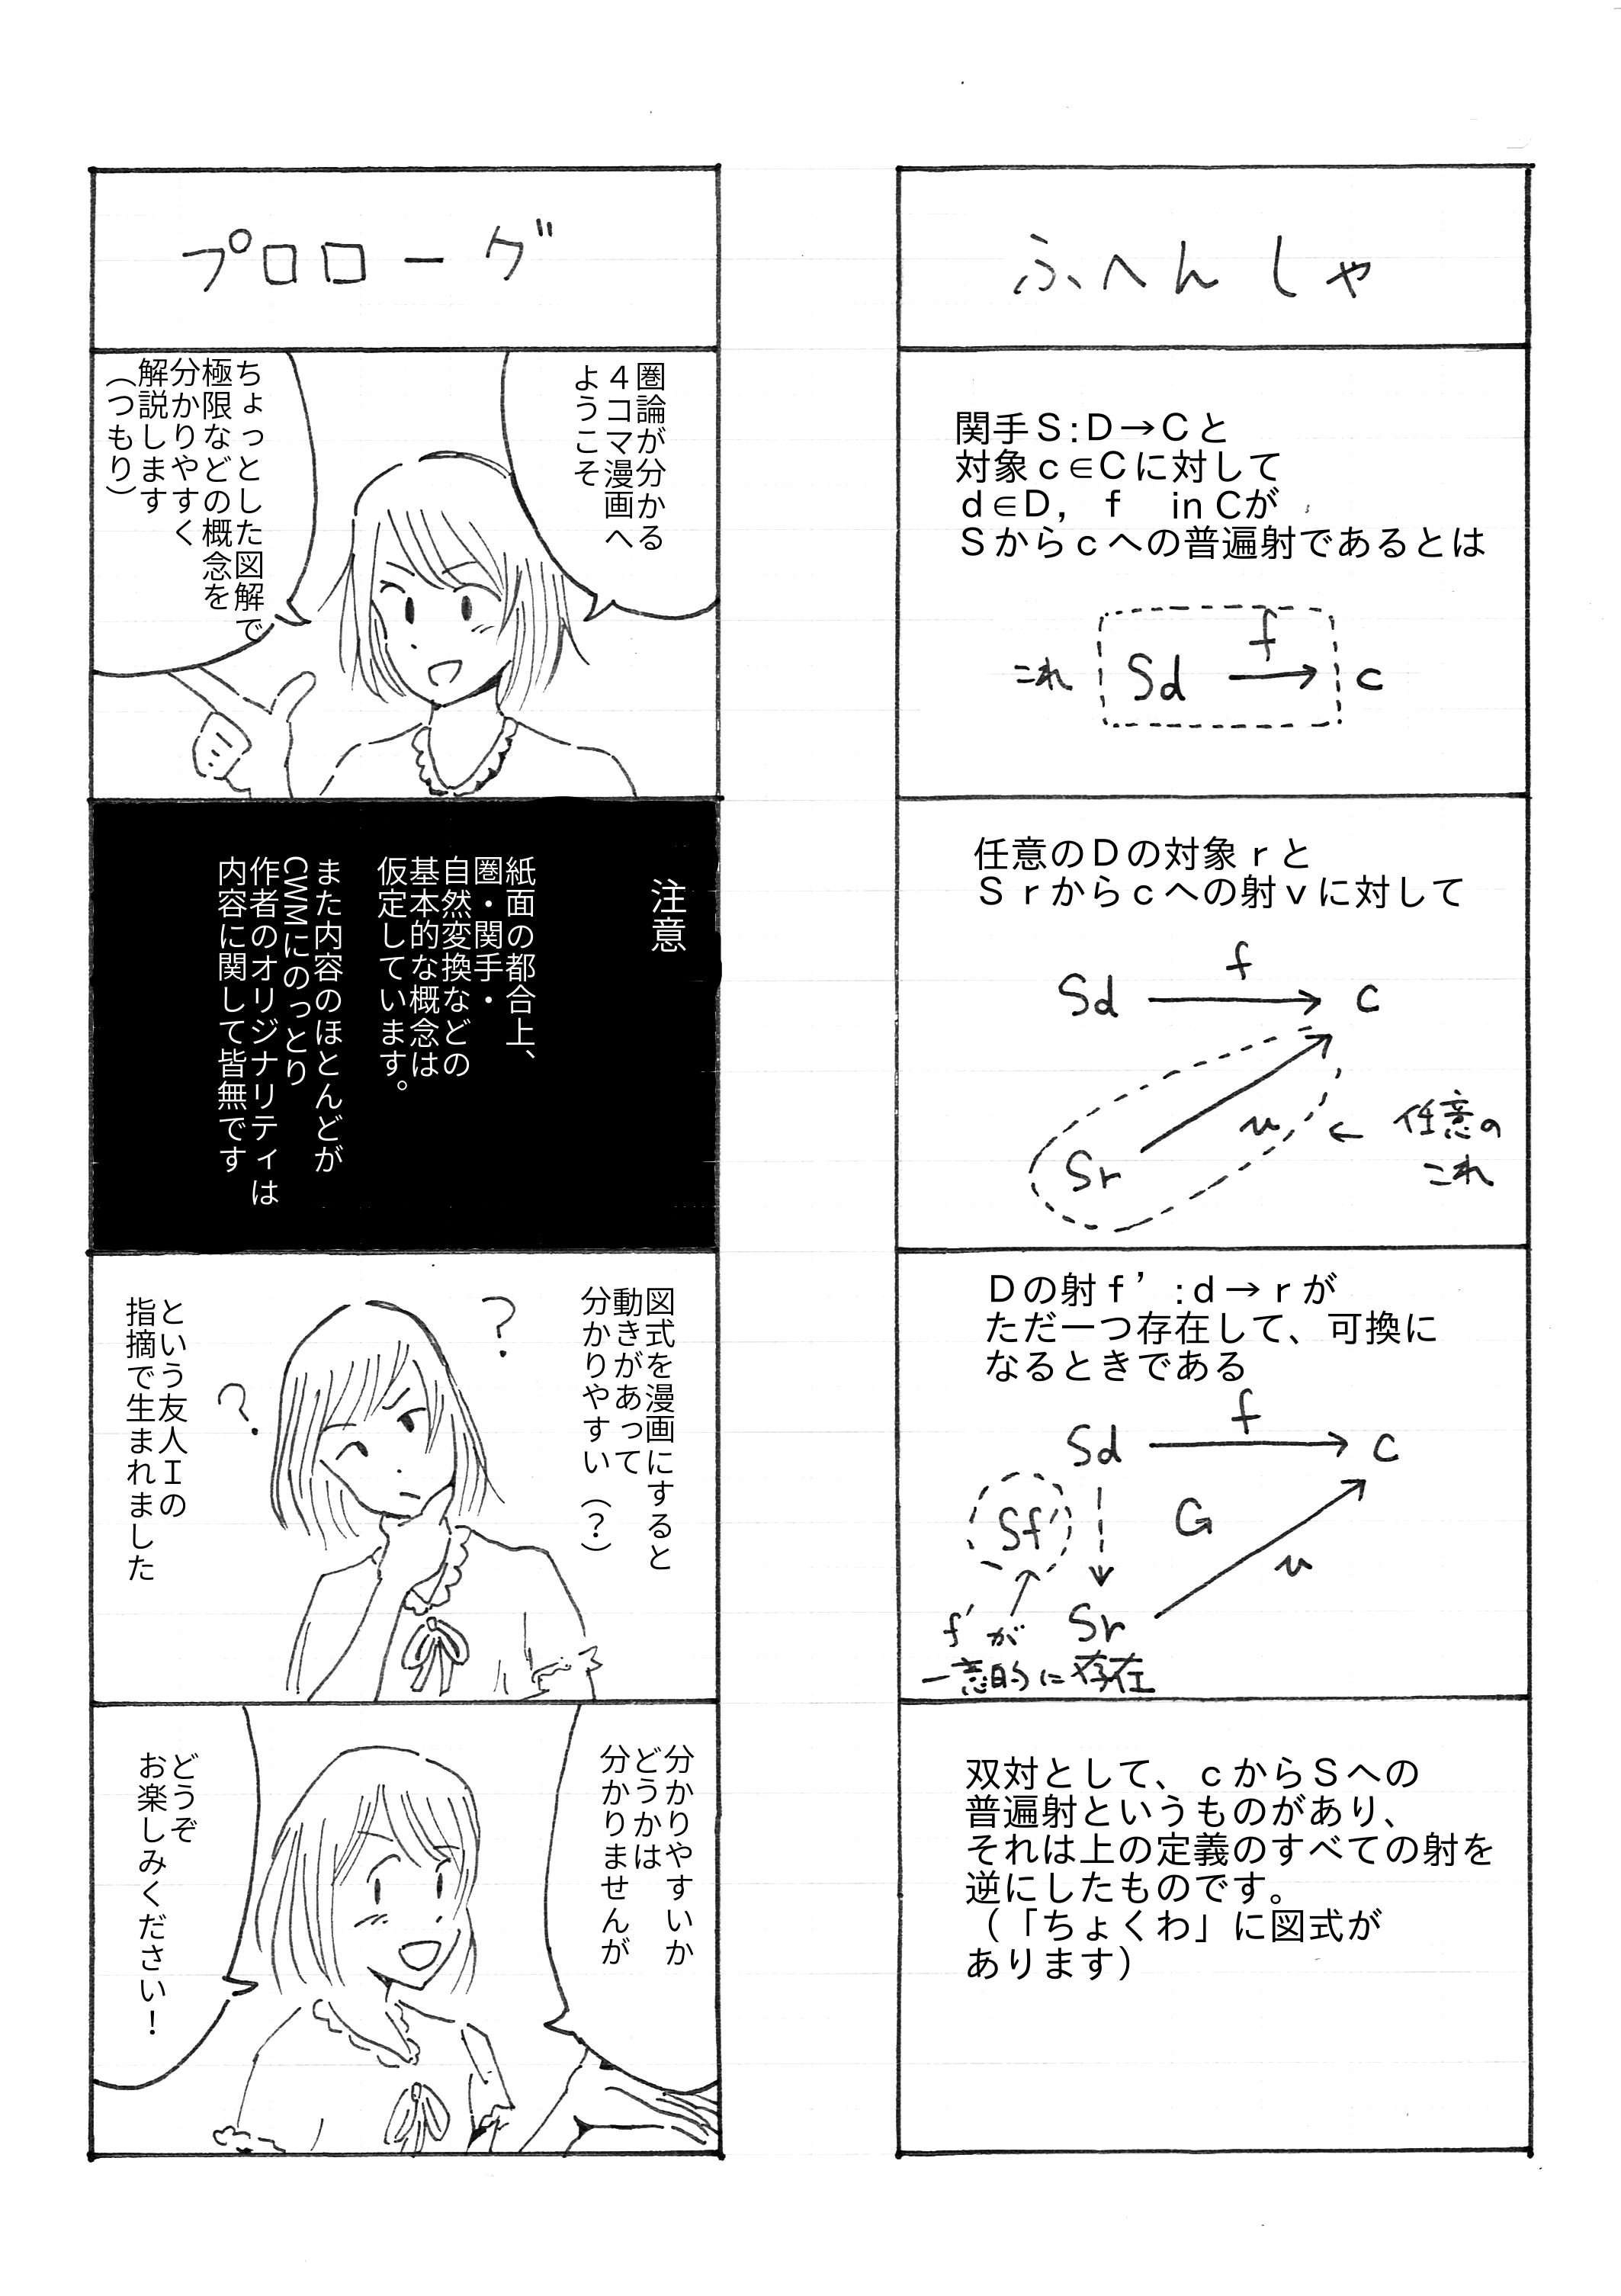
\includegraphics[width=13cm]{kobaken1.png}

\Chapter{トーラスのタイヒミュラー空間I (浅香)}


\Section{序}
形を知りたい―宇宙の形を知りたい,ある特定のタンパク質の形を知りたい―というような欲動はおそらく絶えずあって,調べ始めるにはどの範囲までの形を考えるのか,どの程度似ていたら同じものとみなすのか決めないといけない.ここで考えるのは,複素平面から作られるトーラス全体で,双正則同値になっているものは同じとみなす.さらにトーラスにマーキングをつけて,なお厳しい見方で,マーキングされたトーラスを類別する.このようなトーラス全体が,トーラスのタイヒミュラー空間である.この何を言ってるのか分からない話を分かるように,以下,努力していきたい.もし分からなかったら著者のせいである.

\Section{トーラス}
複素平面からトーラスを作る.複素平面とは,実数だけだと数が足りないために$1$乗して$-1$になる数$i$を加え,実数を拡張したものである.
%
%\begin{wrapfigure}{r}{3cm} 
%\begin{tikzpicture}[domain=-3:3, samples=64, scale=0.8]
%\footnotesize
%    \draw [<->,thick] (0,2) node (yaxis) [above] {Im}
%        |- (3,0) node (xaxis) [right] {Re};
%	\draw (2,1) coordinate (c);
%	\coordinate [label=right:{$2+i$}] (2+i) at (2,1);
%	\draw[dashed] (yaxis |- c) node[left] {$1$} -| (xaxis -| c) node[below] {$2$};
%
%\end{tikzpicture}
%\end{wrapfigure}
\begin{gather*}
(a+bi)+(c+di)=(a+c)+(b+d)i \\
(a+bi)(c+di)=(ac-bd)+(b+d)i \\
\text{($a$, $b$, $c$, $d$ は実数)}
\end{gather*}
と足し算,かけ算が定義され,引き算,割り算もそれから導かれる.
複素平面から何か平行四辺形を切り抜こう.例えば
\begin{center}
\begin{tikzpicture}
\draw (0,0) rectangle (2,1);
\coordinate [label=left:{$0$}] (0) at (0,0);
\coordinate [label=right:{$2+i$}] (2+i) at (2,1);
\end{tikzpicture}
\end{center}
を切り抜くことにする.そして,対辺をそれぞれ貼り合わせると
\begin{center}
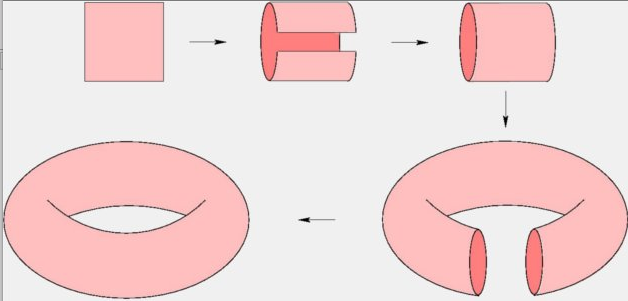
\includegraphics[width=8cm]{asaka3.png}
\end{center}
とドーナツの表面となった.これがトーラスである.

実は切り抜くという操作はあまり良くない.なぜなら数学において境界は大事なのに,切り抜くと境界での構造がぐしゃぐしゃしてしまうからである.余裕のある人はもう少し良いイメージで考えてほしいのだが,それはトイレットペーパーである.切り抜いてしまわずに,複素平面全体をくるくると巻いていく.今回の例で行くと,$0$ と $2$ を結ぶ線分と $i$ と $2+i$ を結ぶ線分がぴたりと一致するように縦に巻き,以降同じ周期でくるくる巻くことにする.複素平面に厚さはないものと考えれば,このように巻ける.複素平面において $0$ と $2$ を結ぶ線分より下にある部分もすでに同じように巻かれていたとする.すると無限に重なった巻物が得られ,さらに $0$ と $i$ を結ぶ線分と $2$ と $2+i$ を結ぶ線分が重なるように横にも周期的に巻いていく.現実の紙だと紙が交差してできないが,この複素平面は自分を通り抜けられると考えれば巻いていける.これによって,平行四辺形が無限個重なったドーナツの表面がえられる.これがトーラスである.

複素平面から作り出したので,トーラスは,詳しくは説明できないが複素平面由来の構造を持っている.このトーラスは長方形の選び方によって形が違う気がする.この話を次の節にもっていく.

\Section{トーラスのモデュライ空間}
トーラスの形が同じであるということを双正則同値によって定める.双正則同値の説明は著者の力量不足のためうまくできない.それでも一応,大雑把に言うと,双正則同値とは,トーラスの持つ複素平面由来の構造が等しいということである.

また,別の言い方をしてみると,2つのトーラス $A$, $B$ に対して,双正則という性質を持つ変換によって $A$ を $B$ に変形できるとき,その2つは双正則であるという.これは,例えば,長方形に対して,相似という関係を,一方を拡大か縮小という変換を行ってもう一方に変形できることと説明するのと同じ言い方である.

双正則同値そのものは難しいが,トーラスをつくる型となった平行四辺形を用いると,双正則同値となる十分条件は説明できる.次の事実がある
\thm
複素平面上に2つの平行四辺形 $A,B$ があったとする.$A$ を縦横比を保ったまま拡大か縮小をして,平行移動と回転移動をすることで $B$ と重なるとき,$A$ からつくられるトーラスと $B$ からつくられるトーラスは双正則同値である
\thmx
\ex
\begin{minipage}{0.5\hsize}
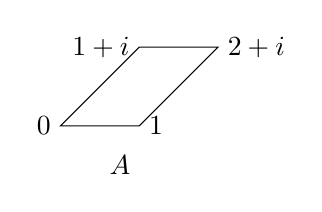
\begin{tikzpicture}
\coordinate [label=left:{$0$}] (A) at (0,0);
\coordinate [label=right:{$1$}](B) at (1,0);
\coordinate [label=left:{$1+i$}](C) at (1,1);
\coordinate [label=right:{$2+i$}](D) at (2,1);
\coordinate [label=right:{$A$}](E) at (0.5,-0.5);
\draw (A) -- (B) -- (D) -- (C) -- cycle;
\end{tikzpicture}
\end{minipage}
\begin{minipage}{0.5\hsize}
\begin{tikzpicture}
\coordinate [label=left:{$1$}] (A) at (0,0);
\coordinate [label=right:{$3$}](B) at (2,0);
\coordinate [label=left:{$3+2i$}](C) at (2,2);
\coordinate [label=right:{$5+2i$}](D) at (4,2);
\coordinate [label=right:{$B$}](E) at (1,-0.5);

\draw (A) -- (B) -- (D) -- (C) -- cycle;
\end{tikzpicture}
\end{minipage} \\
のとき,$A$からつくられるトーラスと$B$からつくられるトーラスは同じものである.
\exx
このことから,$t$は複素平面上の実軸より上の領域(上半平面と名付ける)を自由に動くとして,以下の平行四辺形
\begin{center}
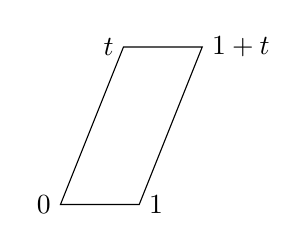
\begin{tikzpicture}
\coordinate [label=left:{$0$}] (A) at (0,0);
\coordinate [label=right:{$1$}](B) at (1,0);
\coordinate [label=left:{$t$}](C) at (0.8,2);
\coordinate [label=right:{$1+t$}](D) at (1.8,2);
\draw (A) -- (B) -- (D) -- (C) -- cycle;
\end{tikzpicture}
\end{center}
を考えれば,他のある位置にある平行四辺形からトーラスをつくったとしても,それに応じて$t$をうまく定めれば, 双正則同値なトーラスをつくれる.すなわち,$t$を動かして,$0$と$1$を結ぶ線分と$0$と$t$を結ぶ線分でできる平行四辺形全体を考えれば,すべてのトーラスは考えつくされる.

このことを踏まえ,さらに次の双正則同値と同値な条件がある.
\thm
\begin{minipage}{0.5\hsize}
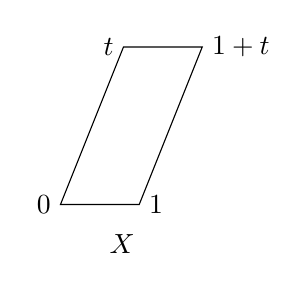
\begin{tikzpicture}
\coordinate [label=left:{$0$}] (A) at (0,0);
\coordinate [label=right:{$1$}](B) at (1,0);
\coordinate [label=left:{$t$}](C) at (0.8,2);
\coordinate [label=right:{$1+t$}](D) at (1.8,2);
\coordinate [label=right:{$X$}](E) at (0.5,-0.5);
\draw (A) -- (B) -- (D) -- (C) -- cycle;
\end{tikzpicture}
\end{minipage}
\begin{minipage}{0.5\hsize}
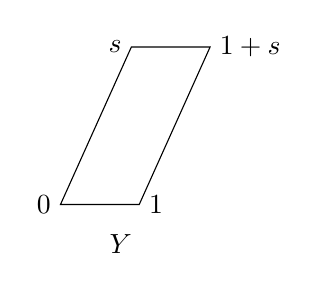
\begin{tikzpicture}
\coordinate [label=left:{$0$}] (A) at (0,0);
\coordinate [label=right:{$1$}](B) at (1,0);
\coordinate [label=left:{$s$}](C) at (0.9,2);
\coordinate [label=right:{$1+s$}](D) at (1.9,2);
\coordinate [label=right:{$Y$}](E) at (0.5,-0.5);
\draw (A) -- (B) -- (D) -- (C) -- cycle;
\end{tikzpicture}
\end{minipage}
$X$と$Y$からつくられるトーラスが双正則同値\\
$\Leftrightarrow \ s=\dfrac {at+b} {ct+d}$をみたす整数 $a$, $b$, $c$, $d$ が存在して,$ad-bc=1$となる
\thmx
\ex
下図の $A$, $B$ によってできるトーラスは双正則同値となる.
実際,\[
\frac{3i-4}{4i-5} = \frac{32+i}{42}
\]
が成り立っている.
\exx
\begin{figure}[h]
\begin{minipage}{0.5\hsize}
\begin{tikzpicture}
\coordinate [label=left:{$0$}] (A) at (0,0);
\coordinate [label=right:{$1$}](B) at (1,0);
\coordinate [label=left:{$i$}](C) at (0,1);
\coordinate [label=right:{$1+i$}](D) at (1,1);
\coordinate [label=right:{$A$}](E) at (0.5,-0.5);
\draw (A) -- (B) -- (D) -- (C) -- cycle;
\end{tikzpicture}
\end{minipage}
\begin{minipage}{0.5\hsize}
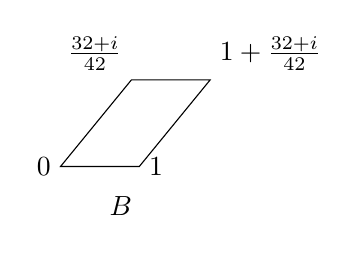
\begin{tikzpicture}
\coordinate [label=left:{$0$}] (A) at (0,0);
\coordinate [label=right:{$1$}](B) at (1,0);
\coordinate [label=above left:{$\frac{32+i}{42}$}](C) at (0.9,1.1);
\coordinate [label=above right:{$1+\frac{32+i}{42}$}](D) at (1.9,1.1);
\coordinate [label=right:{$B$}](E) at (0.5,-0.5);
\draw (A) -- (B) -- (D) -- (C) -- cycle;
\end{tikzpicture}
\end{minipage}
\end{figure}

この関係で互いに等しくならない$t$全体を挙げてみれば,分かったような気になる.これがトーラスのモデュライ空間呼ばれるもので
以下の様なものである.この灰色部分から点$t$をとり,そこから平行四辺形をつくれば,この型を元にトーラスがつくれる.

\begin{minipage}{0.5\hsize}
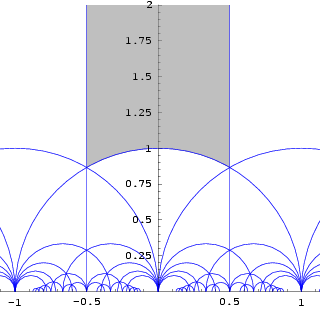
\includegraphics[width=4cm]{asaka8.png}
\end{minipage}
\begin{minipage}{0.5\hsize}
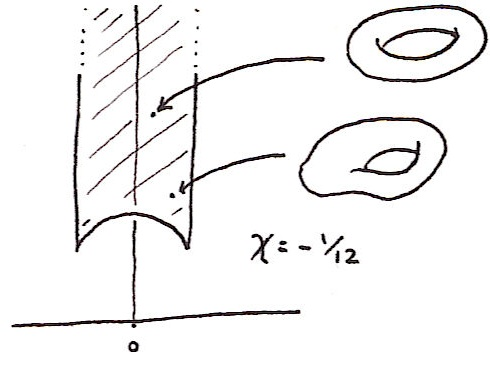
\includegraphics[width=4cm]{asaka9.jpg}
\end{minipage}

つまり,この斜線部上の一点一点がトーラスに対応していて,トーラス全体というものを目の当たりにした.

\Section {トーラスのタイヒミュラー空間}
トーラス上に向きのある輪をおくと
\\
\begin{minipage}{0.5\hsize}
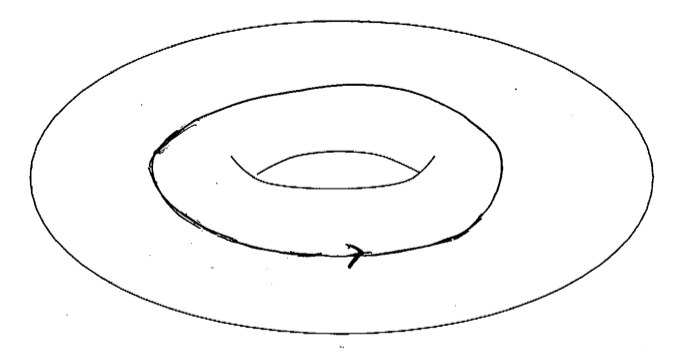
\includegraphics[width=5cm]{asaka10.png}
\end{minipage}
\begin{minipage}{0.5\hsize}
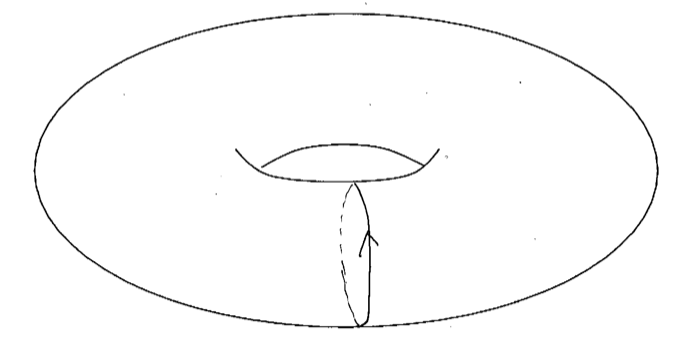
\includegraphics[width=5cm]{asaka101.png}
\end{minipage}
\\
この2つの輪はトーラスから離れてしまわないようにどう伸び縮みさせても一点につぶせない.\\
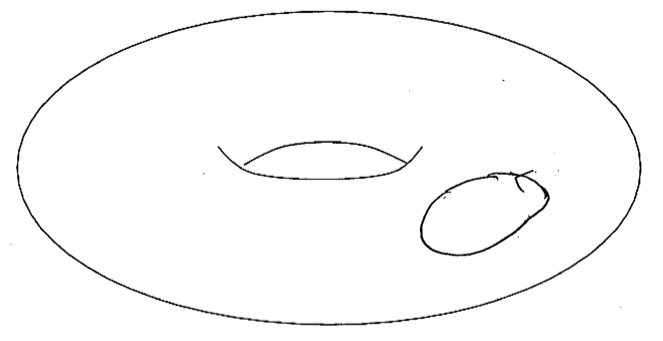
\includegraphics[width=5cm]{asaka11.png}

このような輪はトーラス上で縮めていけば一点につぶせる.

そのような一点につぶせない輪のかけ方はいくらでもある.ただし,トーラス上を移動して,重ねられるような輪のかけ方は同じとみなす.
\\
\begin{minipage}{0.5\hsize}
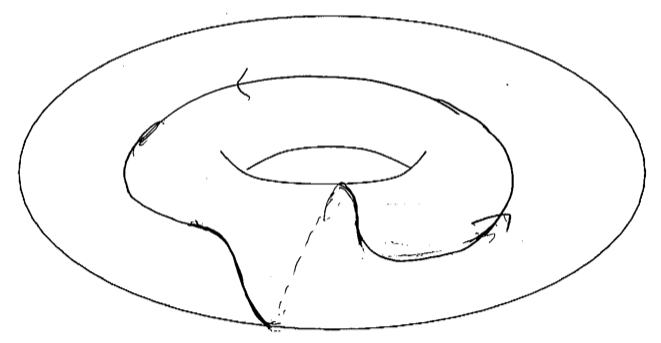
\includegraphics[width=5cm]{asaka12.png}\\
\end{minipage}
\begin{minipage}{0.5\hsize}
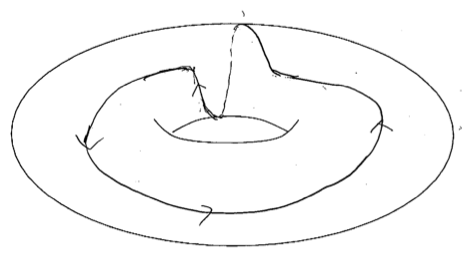
\includegraphics[width=5cm]{asaka121.png}\\
\end{minipage}
\\
この一点につぶせない輪のかけ方は,実は最初の$2$つを組み合わせてすべてつくれる.組み合わせるという言い方はあいまいだが,なんとなくわかって欲しい.

実は最初の$2$つとは別のものからでもあらゆる輪のかけ方を作れる.たとえば\\
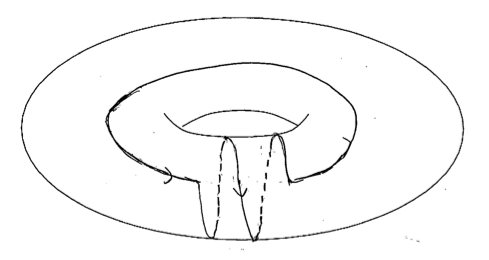
\includegraphics[width=5cm]{asaka14.png}\\
でもよい.この輪のかけ方を生み出す元のものを``基本群の標準生成系''と呼ぶことにする.トーラスを一つ選び,さらにその``基本群の標準生成系''をひとつ選ぶことにする.このトーラスと``基本群の標準生成系''のペアを考える.トーラス全体はどのようなものか,前の章で見た.このトーラス一つ一つに標準生成系とのペアを考えることで種類を増やす.トーラスに標準生成系つけた印をマーキングと呼ぶ.

もう一度tの動く範囲を上半平面として考える.上半平面上のそれぞれ別の場所に $t$, $s$ がいても,前の章で言った条件「$s=\dfrac {at+b} {ct+d}$をみたす整数 $a$, $b$, $c$, $d$ が存在して,$ad-bc=1$となる」を満たせばそこからつくられるトーラスは双正則同値になるのだった.ここで$0$と$1$を結ぶ線分(直線でもよい),$1$と$t$を結ぶ線分(直線でもよい)に注目すると,これらの線分(直線)はトーラス上で,``基本群の標準生成系''となっている.$s$のトーラスについても同じことを考えると``基本群の標準生成系''が得られる.この$2$つのトーラスは「$s=\dfrac {at+b} {ct+d}$をみたす整数 $a$, $b$, $c$, $d$ が存在して,$ad-bc=1$となる」を満たせば,双正則同値になるのだった.つまり,双正則な変換によって$t$のトーラスは$s$のトーラスに変形する.しかし``基本群の標準生成系''はどうかというと,証明は省くが,同じになる($t$のトーラスを$s$のトーラスでうつす変換によって$t$の``基本群の標準生成系''をうつしたものが,トーラス上を動かすことで$s$の``基本群の標準生成系''に一致させられる)とは限らないのだ.今回は,双正則同値になるだけでなく``基本群の標準生成系''も含めて一致するものを同じとみなす厳しい見方を採用する.\\
%\begin{figure}[h]
\begin{minipage}{0.5\hsize}
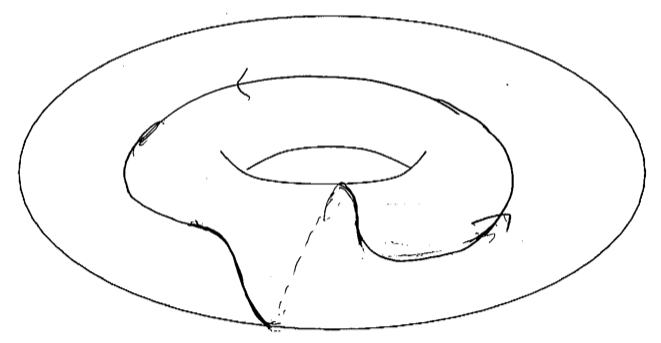
\includegraphics[width=5cm]{asaka12.png}\\
\end{minipage}
\begin{minipage}{0.5\hsize}
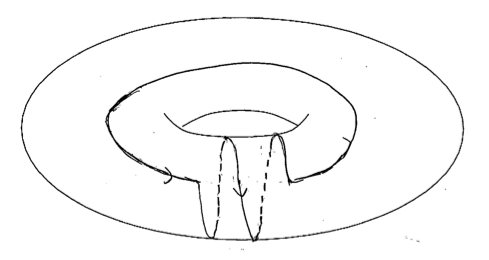
\includegraphics[width=5cm]{asaka14.png}\\
\end{minipage}
%\end{figure}

例えば形は双正則同値でも,次のように左の基本群の標準生成系が右の基本群の標準生成系に写ってしまうような写像はだめなのである.
%\newpage

次の事実がある.
\thm
$X$と$Y$からつくられるマーキングされたトーラスが同じになる\\
$\Leftrightarrow $ $t=s$
\thmx
\begin{figure}[h]
\begin{minipage}{0.5\hsize}
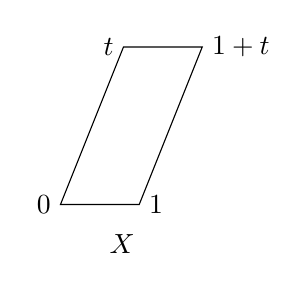
\begin{tikzpicture}
\coordinate [label=left:{$0$}] (A) at (0,0);
\coordinate [label=right:{$1$}](B) at (1,0);
\coordinate [label=left:{$t$}](C) at (0.8,2);
\coordinate [label=right:{$1+t$}](D) at (1.8,2);
\coordinate [label=right:{$X$}](E) at (0.5,-0.5);
\draw (A) -- (B) -- (D) -- (C) -- cycle;
\end{tikzpicture}
\end{minipage}
\begin{minipage}{0.5\hsize}
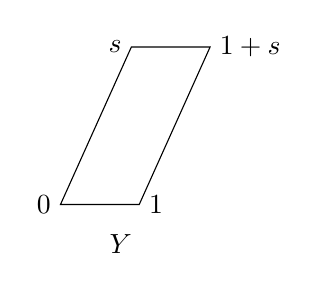
\begin{tikzpicture}
\coordinate [label=left:{$0$}] (A) at (0,0);
\coordinate [label=right:{$1$}](B) at (1,0);
\coordinate [label=left:{$s$}](C) at (0.9,2);
\coordinate [label=right:{$1+s$}](D) at (1.9,2);
\coordinate [label=right:{$Y$}](E) at (0.5,-0.5);
\draw (A) -- (B) -- (D) -- (C) -- cycle;
\end{tikzpicture}
\end{minipage}
\end{figure}
これにより,マーキングされたトーラス全体は上半平面と一致する.この上半平面の一点一点がそれぞれ異なるマーキングされたトーラスに対応する.そして,これがトーラスのタイヒミュラー空間である.
\begin{thebibliography}{9}
\item
難波誠『微分積分学』
(裳華房,1996)
\item
齋藤正彦『齋藤正彦線型代数学』
(東京図書,2014)
\item
斎藤毅『線形代数の世界―抽象数学の入り口』
(東京大学出版会,2007)
\item
森田茂之『講座 数学の考え方〈8〉集合と位相空間』
(朝倉書店,2002)
\item
斎藤毅『集合と位相』
(東京大学出版会,2009)
\item
松本幸夫『多様体の基礎』
(東京大学出版会,1988)
\item
野口潤次郎『複素解析概論』
(裳華房,1993)
\item
楠幸男『函数論―リーマン面と等角写像』
(朝倉書店,2011)
\item
今吉,谷口『タイヒミュラー空間論』
(日本評論社,2004)
\end{thebibliography}

タイヒミュラー空間に関する日本語の本は今のところ[9]しかない.そしてその本までたどりつくには少し長い道のりがある.大学1年で習う解析学と線形代数学の初歩をまず学ばなくてはいけない.前者の一例として[1]を,後者の例として[2], [3]をあげてみた.[2]より[3]の方がより高度に書かれている.そして,大学2年で習う位相については[4], [5]をあげてみた.[4]より[5]の方がまた高度に書かれている.以上を踏まえて大学3年で習う,多様体と複素解析の入門書としてそれぞれ[6], [7]をあげてみた.これらを踏まえ[8]の第4章まで読めれば,[9]の第1章にあるトーラスのタイヒミュラー空間の内容を数学的にきちんと捉えられるのではないかと思う.

数学書はとても多くあるにも関わらず,ごく少ない知識で選んでしまったので,ぜひ自分で書店で選んでみてください.以上です.








\Section{圏論が分かる4コマ漫画2(小林)}
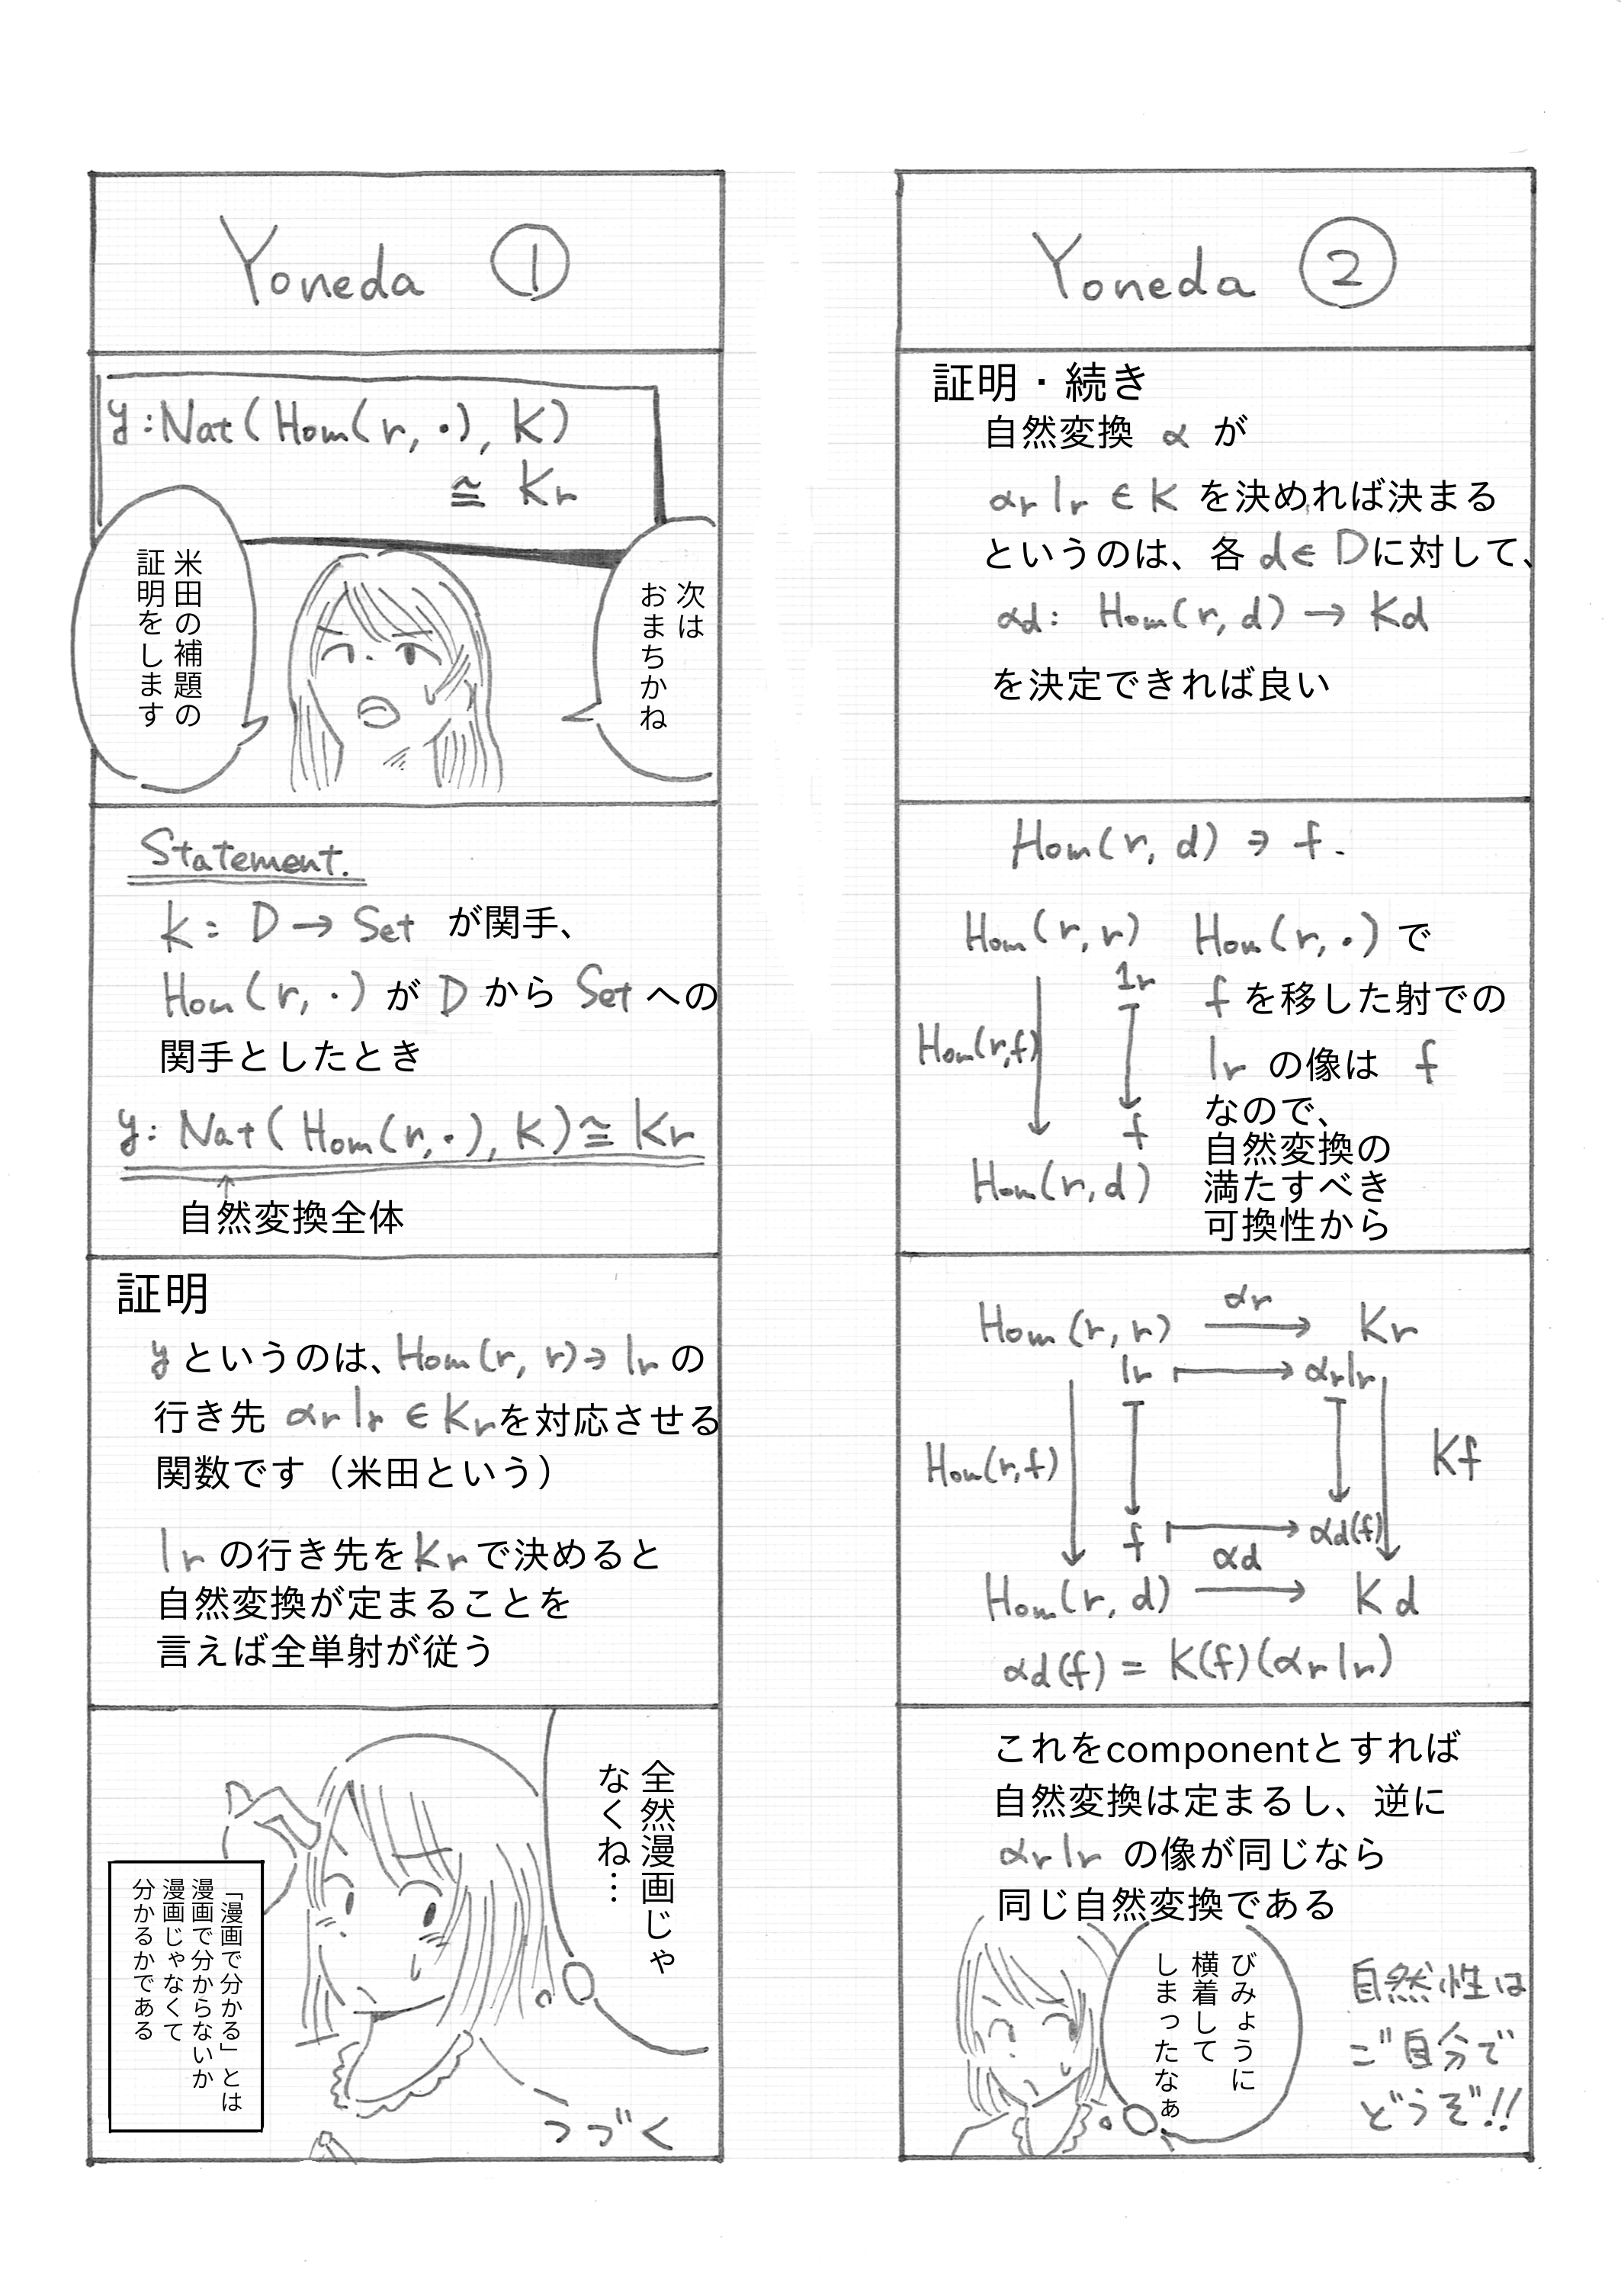
\includegraphics[width=13cm]{kobaken2.png}
\Chapter{フーリエ解析 超入門}
\Section{はじめに}
本日は,数学科展示ますらぼにお越しくださり,また,本冊子$e^{\pi i}sode$を手に取ってくださり,誠にありがとうございます.\\
やっと数理科学研究科棟の空気に慣れ始めた私ですが,数学の世界というものは想像よりもはるかに広く,毎日が苦労の連続です.そんな日々だからこそ,今まで知らなかった世界が見えてくる,視界が広がっていく時の感動は一入です.\\
本冊子のテーマは「わたしのえぴそーど」ということで,私が高校生のときに初めて学んだフーリエ解析について少しだけ紹介したいと思います.私が初めて学んだ時の感動を多くの人と共有したいので,できるだけ平易な内容で(高校数学くらいを前提として),「こんな方法があるんだ」といったことを知って頂くような,そんな記事にするつもりです.

\Section{基礎知識}
高校1年生になると,いわゆる「サインコサイン」を学ぶと思います.高校の数学と言えば「サインコサイン」と「ビブンセキブン」というのが,語呂の良さなどもあって数学が苦手な学生の敵にされがちです.\\
高校2年生で,関数$\sin x$と$\cos x$を学びます.直角三角形から生み出された「サインコサイン」を拡張した概念です.ご存じ,周期$2 \pi$で1と-1の間をウロウロ振動する関数です.\\
$\sin 2x$,$sin 3x$,…を考えると,これはだんだん周期が短くなります.$2\sin x$,$3\sin x$,…を考えると,振動の振幅がだんだん大きくなります.
これらの関数について微分・積分を考えることが出来ます.また,これらの関数を掛け合わせて積分したものについて,以下の関係式が成り立ちます.

\[
\int_{-\pi}^\pi \sin mx \sin nx dx = 0
\]
(m,nは整数,$m \neq n$)

\[
  \int_{-\pi}^\pi \sin mx \sin nx dx = \pi
\]
(m,nは整数,$m = n$)\\


つまり,$\sin x$の関数の周期のなかで,振動の回数が違う二つのサイン関数を掛け合わせて積分すると0になり,同じ振動数の関数どうしを掛け合わせると$\pi$になります.この積分は,加法定理から導かれる
$\sin x \sin y = \frac{1}{2} (\cos(x-y)-\cos(x+y))$
から計算できます.\\
$\cos x$についても同じ関係式が成り立ちます.
さらに,$\sin x$と$\cos x$を掛け合わせて積分すると,mとnが整数なら同じ値でも違う値でも,

\[
  \int_{-\pi}^\pi \sin mx \cos nx dx = 0
\]

が成り立ちます.

\Section{フーリエ級数}
以上の前提を踏まえてフーリエ級数を定義します.\\
フーリエ級数はざっくり言うと,「『まともな』関数ならば,無限個の三角関数の足し合わせで表現できる」といった考え方です.数式で表現すると以下のようになります.

\[
  f(x) = \sum_{n=1}^\infty (a_n \cos nx + b_n \sin nx + C)
\]

さらっと一つの式でまとめましたが,これは大層なことを言っていて,つまり直線でも放物線でも,どんな関数でもサインとコサインを足し合わせ続ければ再現できるということなのです!\\
『まともな』関数と言いましたが,例えば有理数に対して1を,無理数に対して0を返すような関数はこのような展開が出来ません.最低限の条件として,関数が区部的$C^1$級,つまりはいくつかの点で関数を区切った時にそれぞれのパーツが微分可能であれば構いません.高校までで習うほとんどの関数なら大丈夫なのです.\\

さて,本当に表されるのであれば,各係数$a_n,b_n,C$は先程の積分の結果を使えば簡単に求められます.
$k$を整数として,両辺に$\cos kx$をかけて積分します.

\[
  \int_{-\pi}^\pi f(x) \cos kx = \sum_{n=1}^\infty (a_n \cos nx \cos kx+ b_n \sin nx \cos kx + C \cos kx)
\]

そうすると,右辺は$\cos kx \cos kx$の積分だけが1となって残り,残りは先程の計算で0になってしまいます.$\sin nx \cos kx$の積分も消えて,$\cos kx$の積分も一周期分の積分のため消えてしまいます.したがって,

\[
  \frac{1}{\pi} \int_{-\pi}^\pi f(x) \cos kx dx = a_k
\]

が出てきて,すべてのnについて係数(フーリエ係数)がわかります.
また,$sin kx$をかけたり,そのまま積分することで,

\[
  \frac{1}{\pi} \int_{-\pi}^\pi f(x) \sin kx dx = b_k
\]

\[
  \frac{1}{2 \pi} \int_{-\pi}^\pi f(x) dx = C = \frac{a_0}{2}
\]

が導かれます.\\
また,オイラーの公式\\
$e^{ix} = \cos x + i \sin x$\\
を用いると,フーリエ級数は以下のように簡単に書き換えることもできます.

\[
  f(x) = \sum_{n=-\infty}^\infty c_n e^{inx}
\]

\[
  c_n = \frac{1}{2\pi} \int_{-\pi}^\pi f(x) e^{-inx} dx
\]

\Section{フーリエ級数の収束}
とりあえず,級数が収束するなら$a_n,b_n,C$が決定することは分かりました.問題は本当に収束するのかどうかです.\\
数学が得意な人にとってはここが一番気になるところだと思いますが,誌面の都合上,証明の流れだけお話しようと思います.\\

fの定義域の点xにおいて,右側から近づけた極限$f(x+0)$と,左側から近づけた極限$f(x-0)$について考えます.また,
\[
  S_N[f](x) = \sum_{n=-N}^N c_n e^{inx}
\]
とおきます.これはフーリエ級数の足し合わせをN番目まで行ったものです.\\
$I_N = S_N[f](x) - \frac{1}{2}(f(x+0)+f(x-0))$とおき,
\[
  \lim_{N \to \infty} I_N = 0
\]
を示せば,fがxで連続ならばfをフーリエ級数展開したときに収束してくれることが示せます.\\
ここで,$I_N$を分解します.分解のために以下の関数を定義します.\\
$D_N(x) = \frac{\sin(N + \frac{1}{2})x}{\sin(\frac{x}{2})}$\\
これをディリクレ核と呼びます.これを用いると,$I_N$を分解して,
\[
  I_N = (\frac{1}{2\pi} \int_{-\pi}^0 f(x+t) D_N(t) dt - \frac{1}{2} f(x-0)) +  (\frac{1}{2\pi} \int_0^\pi f(x+t) D_N(t) dt - \frac{1}{2} f(x+0))
\]
とできます.あとは前半部と後半部がそれぞれ収束することを示せばよいです.\\
尻切れトンボになってしまい申し訳ありませんがここまでにします.本当は$D_N(x)$の性質からディリクレ核の積分などを補題として使い,これらが収束することを示すのですが,興味がある人は是非調べてみてください,と言いつつ丸投げします.

\Section{私が高校生だったころのフーリエ級数}
いま求めたフーリエ級数ですが,何に使えるのか,という疑問は当然出てきます.\\
ひとつとしては,すべての関数が基本となる波の足し合わせと言っているのだから,例えば任意の種類の音を基本となる音だけ用いて再現することが可能になります.さらに熱方程式の解の導出にも表れ,物理や工学の世界で大きく発展できそうです.\\
しかし,当時この手法を知ったころの私が惹かれたのは,むしろ副産物の方でした.\\
いま,$f(x) = x^2$ としてフーリエ級数を計算します.この時,この関数を$({-\pi} \leq x \leq \pi)$に制限し,$(x \leq -\pi)$や$(x geq \pi)$同じ${2\pi}$周期で何度も同じ放物線が現れるようにします.\\

\begin{figure}[h]
  \begin{center}
    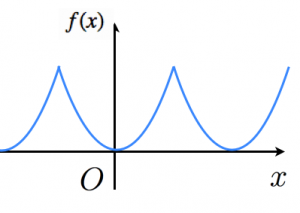
\includegraphics[clip,width=7.0cm]{osawa.png}
    \caption{放物線(周期$2\pi$)}
    \label{f_para}
  \end{center}
\end{figure}

フーリエ係数を求めると,
\[
  \frac{a_0}{2} = \frac{1}{\pi} \int_{-\pi}^\pi x^2 dx = \frac{\pi^2}{3}
\]

\[
  a_n = \frac{1}{\pi} \int_{-\pi}^\pi x^2 \cos nx dx = (-1)^n \frac{4}{n^2}
\]

また,fは偶関数(y軸について対称)である.$\cos nx$は同様に偶関数なので足し合わせても差し支えは無いが,$\sin nx$を足し合わせてしまうと,これは奇関数なので,足し合わせてしまうと結果が偶関数でなくなってしまう.
したがって,$b_n = 0$が成り立つ.\\
つまり,

\[
  f(x) = x^2 = \frac{\pi^2}{3} + \sum_{n=1}^\infty (-1)^n \frac{4}{n^2} \cos nx
\]

ここで,$x = \pi$を代入すると,

\[
  \pi^2 = \frac{\pi^2}{3} + \sum_{n=1}^\infty \frac{4}{n^2}
\]
が成り立ち,整理すると

\[
  \sum_{n=1}^\infty \frac{1}{n^2} = \frac{\pi^2}{6}
\]

となります.これは,自然数の2乗の逆数を足し合わせた時の極限になります.\\

無限級数の和として,無限等比級数は高校数学の範囲で求められますが,$\sum_{n=1}^\infty \frac{1}{n^2}$については求められませんでした.しかしフーリエ級数を使えば,副産物としてこのような極限が求められるのです.\\
さらに別の関数を使えばこのような極限も求められます.
\[
  \sum_{n=1}^\infty \frac{1}{n^4} = \frac{\pi^4}{90}
\]
\[
  \sum_{n=1}^\infty \frac{1}{n^6} = \frac{\pi^6}{945}
\]

この,$\sum_{n=1}^\infty \frac{1}{n^p} = \zeta(p)$はゼータ関数といい,複素数に拡張することが出来ます.ゼータ関数の零点についての主張が,かの有名なリーマン予想というわけです.\\


\Section{フーリエ変換}
先のフーリエ級数では周期$2\pi$の関数を扱いましたが,世の中の関数の周期は$2\pi$だけとはいきません.さらに周期$L$の関数を考え,$L$が無限大のときを考えれば,周期関数以外でもこの手法が役に立ちそうです.\\
周期$2L$の関数のフーリエ級数は,変数変換などを使って以下のように表されます.
\[
  f(x) = \sum_{n=-\infty}^\infty c_{L,n}(f) e^{inx\pi/L}
\]
\[
  c_{L,n} = \frac{1}{2L} \int_{-L}^L f(y) e^{-iny\pi/L} dy
\]
ここで,$\Delta\xi = \frac{\pi}{L},{\xi_k} = \frac{k\pi}{L}$とおきます.
\[
  f(x) = \sum_{n=-\infty}^\infty c_{L,n}(f) e^{i{\xi_k}x} \frac{\Delta\xi}{\Delta\xi}
  =\frac{1}{2\pi} \sum_{n=-\infty}^\infty 2{L}(\frac{1}{2L} \int_{-L}^L f(y) e^{-i{\xi_k}y} dy) e^{i{\xi_k}x} {\Delta\xi}
\]
ここで,$L \to \infty$のときを考えると,${\Delta\xi} \to 0$になるが,このときリーマン積分の定義より総和が積分に置きかわります.
\[
  f(x) = \frac{1}{2\pi} \int_{-\infty}^\infty (\int_{-\infty}^\infty f(y) e^{-i\xi y}dy) e^{i\xi x}d\xi
\]

2つの積分操作が為されていますが,それぞれを関数の変換とみなして以下のように表現します.

\[
  \mathcal{F}[f](\xi) = \int_{-\infty}^\infty e^{-ix\xi} f(x) dx
\]
\[
  \mathcal{F}^{-1}[f](x) = \frac{1}{2\pi} \int_{-\infty}^\infty e^{ix\xi} f(\xi) d\xi
\]

上をフーリエ変換,下をフーリエ逆変換といいます.フーリエ級数を拡張した時の式から,フーリエ変換をしたあとにフーリエ逆変換をすると元の関数に戻ることがわかります.\\
フーリエ変換の面白いところは色々ありますが,例えば元の関数に微分操作,積分操作を行うとフーリエ変換は以下のように書き換わります.\\
\[
  \mathcal{F}[\frac{df(x)}{dx}](\xi) = i\xi \mathcal{F}[f](\xi)
\]
\[
  \mathcal{F}[\int_{-\infty}^x f(y) dy](\xi) =\frac{1}{i\xi} \mathcal{F}[f](\xi)
\]
これは,例えば微分方程式や積分方程式を解くときに,フーリエ変換をして微分操作や積分操作を掛け算に直してから計算し,フーリエ逆変換で戻せば解が求められることを意味しています.このフーリエ変換や,ラプラス変換と呼ばれる別の変換は,このように関数に対する操作を簡単にしてくれます.こうしてフーリエ級数を発展させて,関数の変換を導出しました.

\Section{おわりに}
以上,フーリエ級数とフーリエ変換について簡単にですが紹介しました.\\
これらフーリエ解析については,東大の数学科では3年の秋〜冬に学習します.フーリエ変換は工学の世界で頻繁に出てくるので,工学部では数学科より早く学ぶのですが,数学科ではルベーグ積分の基礎をきちんと学習してからフーリエ解析に入り,収束の証明をきちんと行います.\\
この冊子の中では比較的平易な内容ではありますが,私が出会ったときに一番好奇心を掻き立てられたのがこの単元だったので,「わたしのえぴそーど」というタイトルにふさわしいと思い紹介しました.\\
ぜひ「ますらぼ」で,それから今後もいろいろな機会で,数学の世界に触れていただければと思います.
\begin{thebibliography}{9}
\item 新井 仁之 「新・フーリエ解析と関数解析学」 培風館\\
\item 竹内 淳 「高校数学でわかるフーリエ変換」 講談社ブルーバックス\\
\end{thebibliography}

文責:大澤 哲史

\Chapter{非可換幾何の呼び声(TN)}
\Section{はじめに}
 いきなりで申し訳ないのですが,本稿で非可換幾何学の理論を展開することはありません.タイトル詐欺もいいところですが,幾何と作用素環の間の対応を見て,そこから非可換幾何への着想を紹介いたします.\\
 数学において,調べたい対象を別の何かと対応付け,対応付けたものを調べることで元の調べたい対象の性質がわかるようになる,ということはしばしばあります.例えば,それなりに良い性質を持つ幾何的な対象である局所コンパクトハウスドルフ空間というものを考えます.例えば,我々の住む空間である(と思われる)3次元実空間$\mathbb{R}^3$などがその例です.数直線や2次元平面も(通常の位相を考えれば)局所コンパクトハウスドルフ空間とみなせます.さて,この局所コンパクトハウスドルフ空間の上で連続関数を定義することができます.そのような連続関数すべてを集めてくると,その集合には関数の和と積,それから複素数倍を考えることができ,数学で「多元環」,「代数」などという構造が入ります.これを連続関数環といいますが,この代数的な「環」(正確には多元環)を調べることにより,元の空間の性質がよくわかる,ということが知られています.\\
 この連続関数環は実は$C^*$-環というものの1つです.$C^*$-環はHilbert空間上の有界線型作用素のなす多元環ですが,その中でも可換(積の順序が交換可能)なもので,実は可換な$C^*$-環はある局所コンパクト空間上の連続関数環になります.従って一方を調べることはもう一方を調べることになります.\\
 このような対応がありますが,$C^*$-環は可換なものだけでなく非可換なものがたくさん(それはもうたくさんです)あります.では,その非可換な$C^*$-環が対応しているであろう「非可換」な「空間」はどういったものなのでしょうか?\\
 今回の記事ではこのようなお話について紹介させていただきます.なお,話題の紹介を優先したため,また紙面と執筆者の気力の都合もあり証明は省略しました.(興味を持っていただけた方は参考文献を参照してください)
\Section{$C^*$-環}
 以下では少々式を用いて作用素環論の基礎を述べる.よくわからないという方は流し読みで雰囲気だけでも感じてもらえると幸いである.
\Subsection{Banach空間,Hilbert空間}
 線形空間$A$にノルム$\parallel x\parallel$(まぁ,絶対値みたいなものです)が定義されていて,そのノルムに関して完備である,すなわち
\begin{center}
Cauchy列$\{ x_n\}_{n \in \mathbb{N}},\lim_{m,n \rightarrow \infty}\parallel x_m-x_n\parallel =0$に対し\\
その極限が存在する:$\lim_{n\rightarrow \infty}\parallel x_n-x\parallel=0$
\end{center}
をみたすとき,$A$を$\textgt{Banach空間}$という.\\
 同様に線形空間に内積が定義され(pre-Hilbert空間,計量線形空間などという),内積について完備であるとき,Hilbert空間という.
 $ex)$ 2次元実ベクトル全体の空間
\begin{center}
$\Biggl\{ \left(
\begin{array}{c}
a \\
b \\
\end{array}
\right)\Biggl|a.b\in \mathbb{R}\Biggr\}$
\end{center}
に和と実数倍を通常のベクトルの和と実数倍で定め,ノルムを通常のベクトルの長さで定めると,これはBanach空間である.\\
\Subsection{$C^*$-環の定義}
 $A$をBanach空間とする.Aに積$A \times A \ni \left(x,y\right) \mapsto xy \in A$,写像$A\ni a \mapsto a^*\in A$が定義され,以下の条件を満たすとき,$A$を\textgt{$C^*$-環}という.
\begin{itemize}
\item $A$は和と積について$\mathbb C$上の多元環である.つまり,積について結合法則と分配法則が成り立つ.
\item $\parallel xy\parallel \leq \parallel x\parallel \parallel y\parallel$
\item $\left(x^*\right)^*=x$
\item $\left(x+y\right)=x^*+y^*$
\item $\left(xy\right)^*=y^*a^*$
\item $\left(\alpha x\right)^*=\overline{\alpha} x^*$
\item $\parallel x^*\parallel=\parallel x\parallel$
\item $\parallel xx^*\parallel=\parallel x\parallel \parallel x^*\parallel$
\end{itemize}
写像$*:a \mapsto a^*$を\textgt{対合}という.$C^*$-環$A$の積が可換であるとき,$A$は\textgt{可換}であるという.また,$A$が積について単位元をもつとき,$A$は\textgt{unital}であるという.
\Subsection{*-準同型写像}
 $A,B$を$C^*$-環とする.写像$\pi:A \rightarrow B$が
\begin{center}
$\pi \left( x+y\right)=\pi \left( x\right)+\pi \left( y\right), \pi \left( xy\right)=\pi \left( x\right)\pi \left( y\right)$
$\pi \left( \lambda x\right)=\lambda \pi \left( x\right) \lambda \in \mathbb{C}$
$\pi \left(x^*\right)=\pi \left(x\right)^*$
\end{center}
をみたすとき,$\pi$は\textgt{*-準同型}であるという.$\pi $が全単射*-準同型であるとき,$\pi$は同型であるという.$C^*$-環$A,B$の間に同型$\pi$が存在するとき,$A,B$は\textgt{同型}であるといい,$A\simeq B$と表す.
\Subsection{$C^*$-環の直和}
$\{A_{\lambda}\}_{\lambda \in \Lambda}$を$C^*$-環の族とする.これに対し,集合$A$を
\begin{center}
$A=\{ \left( x_{\lambda}\right)_{\lambda \in \Lambda}|\forall x_{\lambda}\in \Lambda ,
\sup_{\lambda \in \Lambda}<\infty \}$
\end{center}
で定める.$A$に和と積,スカラー倍,及びノルムを
\begin{itemize}
\item $\left( x_{\lambda}\right)_{\lambda \in \Lambda}+\left( y_{\lambda}\right)_{\lambda \in \Lambda}
=\left( x_{\lambda}+y_{\lambda}\right)_{\lambda \in \Lambda}$
\item $\left( x_{\lambda}\right)_{\lambda \in \Lambda}\left( y_{\lambda}\right)_{\lambda \in \Lambda}
=\left( x_{\lambda}y_{\lambda}\right)_{\lambda \in \Lambda}$
\item $\alpha \left( x_{\lambda}\right)_{\lambda \in \Lambda}=\left( \alpha x_{\lambda}\right)_{\lambda \in \Lambda}$
\item $\parallel \left( x_{\lambda}\right)_{\lambda \in \Lambda}\parallel=\sup_{\lambda \in \Lambda}\parallel x_{\lambda}\parallel$
\end{itemize}
で定めると,これは$C^:$-環である.$A$を$\{A_{\lambda}\}_{\lambda \in \Lambda}$の\textgt{直和}といい,
\begin{center}
$A=\sum_{\lambda \in \Lambda} \oplus A_{\lambda}$
\end{center}
と表す.
\Subsection{重要な$C^*$-環の例}
 $\Omega$を局所コンパクト空間とする.$C_{\infty}\left( \Omega\right)$を無限遠で消える$\Omega$上の連続関数全体の集合とする.これに和・スカラー倍と積,対合,ノルムを
\begin{itemize}
\item $\left(\lambda x+\mu y\right)\left(\omega\right)=\lambda x\left(\omega\right)+\mu y\left(\omega\right)$
\item $\left(xy\right)\left(\omega\right)=x\left(\omega\right)y\left(\omega\right)$
\item $x^*\left(\omega\right)=\overline{x\left(\omega\right)}$
\item $\parallel x\parallel=\sup\{|x\left(\omega\right)||\omega \in \Omega\}$
\end{itemize}
で定めると,$C_{\infty}\left( \Omega\right)$は可換$C^*$-環である.$\Omega$がコンパクトであるとき,かつその時に限り$C_{\infty}\left( \Omega\right)$はunitalである.\\
\\
 ※局所コンパクト空間$\Omega$上の連続関数$x$が\textgt{無限遠で消える}(\textgt{vanishing at infinity}):任意の正数$\epsilon >0$に対し,あるコンパクト集合$K\subset \Omega$が存在して,
\begin{center}
$\forall \omega \in \Omega\setminus K,\parallel x\left( \omega\right)\parallel<\epsilon$
\end{center}
が成り立つ.
\Section{Gelfand表現}
\Subsection{指標}
 $A$を可換$C^*$-環とする.写像$\pi:A\rightarrow\mathbb{C}$が0写像でなく,$A$から$\mathbb{C}$への*-準同型であるとき,$\pi$を$A$の\textgt{指標}といい,$A$の指標全体を$\Omega\left(A\right)$で表し,\textgt{指標空間}という.
 $\Omega\left(A\right)$に弱*位相,すなわち,$A$を$A^{**}$の部分空間として考えた時に,各$x\in A$を連続にする$\Omega\left(A\right)$上の位相であって,和,積,スカラー倍を連続にするようなもののうち最弱なものとする.すると,この位相に関し,$\Omega\left(A\right)$は局所コンパクトHausdorff空間になる.さらに,$A$がunitalならば$\Omega\left(A\right)$はコンパクトである.
\Subsection{Gelfand表現}
 写像$\mathscr{F}:A \rightarrow C_{\infty}\left(\Omega\left(A\right)\right)$を
\begin{center}
$\mathscr{F}\left(x\right)\left(\pi\right)=\pi\left(x\right)$
\end{center}
で定める.$\mathscr{F}$を$A$の\textgt{Gelfand表現}という.
\Subsection{Gelfand-Naimarkの定理その1}
\begin{theo}
$A$を可換$C^*$-環とする.$A$の{\rm Gelfand}表現$\mathscr{F}$は$A$から$C_{\infty}\left(\Omega\left(A\right)\right)$への等距離*-同型である.
\end{theo}
 このGelfand-Naimarkの定理により,任意の可換$C^*$-環に対し,ある局所コンパクトハウスドルフ空間上の連続関数環が対応することがわかった.実は局所コンパクトハウスドルフ空間上の連続関数環から元の位相空間を復元することができるので,この定理は可換$C^*$-環から局所コンパクトハウスドルフ空間を構成できることを示している(その逆も然り).すなわち\textgt{,可換$C^*$-環の理論は局所コンパクト(ハウスドルフ)空間の理論と等価}とみなしてよいということである.(余談ではあるが,圏論の言葉を用いれば,局所コンパクトハウスドルフ空間の圏と可換$C^*$-環の圏が圏同値である,ということである)\\
 かくして可換$C^*$-環と局所コンパクト空間という幾何学的な概念が繋がった.この定理はGrothendieckのスキーム論にも影響を与えたと言われている.\\
 では,この定理から可換ではない$C^*$-環も何か幾何学的なものに対応しているのではないか,と考えてみる.それはどんなものであろうか.可換$C^*$-環から局所コンパクトハウスドルフ空間を構成できるならば、同じ手続きによって非可換な$C^*$-環から「空間」を構成できるののではないだろうか.それはもはや「点」や「空間」といった概念が意味を成すのかわからないが,ともかく非可換$C^*$-環により「構成」した「空間」に相当する何かを「非可換空間」ということにしよう.「非可換空間」は$C^*$-環から構成されるので,関数環側から微分構造やRiemann計量を導入する方法がわかれば,非可換微分多様体や非可換Riemann多様体が考えられる.「非可換空間」について知るためにはその基となる非可換な$C^*$-環について知らねばなるまい.そこで,もう少し一般の可換とは限らない$C^*$-環について調べていく.
\Section{GNS表現}
\Subsection{$C^*$-環の表現}
 $A$を(可換とは限らない)$C^*$-環,$\mathfrak{H}$をHilbert空間とする.*-準同型$\pi:A\rightarrow \mathcal{B}\left(\mathfrak{H}\right)$に対し,対$\left(\pi,\mathfrak{H}\right)$をAの\textgt{表現}という.$\pi$が単射であるとき,表現$\left(\pi,\mathfrak{H}\right)$は\textgt{忠実}であるという.
\Subsection{表現の直和}
 $C^*$-環$A$の表現の族$\left(\pi_{\lambda},\mathfrak{H}_{\lambda}\right)_{\lambda \in \Lambda}$を考える.$\mathfrak{H}_{\lambda}$の直和Hilbert空間を,$\mathfrak{H}$;
\begin{center}
$H:=\bigoplus_{\lambda \in \Lambda}\mathfrak{H}_{\lambda}$
\end{center}
とする.これに対し,表現の\textgt{直和}$\left(\pi,\mathfrak{H}\right)$を
\begin{center}
$\pi\left(x\right)\left(\left(\xi_{\lambda}\right)_{\lambda \in \Lambda}\right):=
\left(\pi_{\lambda}\left(x\right)\xi_{\lambda}\right)_{\lambda \in \Lambda}$
\end{center}
で定める.
\Subsection{状態}
 $A$を(可換とは限らない)$C^*$-環とする.$A$の線型汎函数$\omega:A\rightarrow \mathbb{C}$が
\begin{center}
$\forall x\in A,\omega \left(x^*x \right)\geq0$
\end{center}
をみたすとき,$\omega$を\textgt{正線型汎函数}という.正線型汎函数は有界線型作用素である.$\parallel\omega\parallel$=1をみたす正線型汎函数を\textgt{状態}という.
\Subsection{GNS表現の構成}
 $A$を(可換とは限らない)$C^*$-環とする.$A$の正線型汎函数$\omega:A\rightarrow \mathbb{C}$が与えられたとき,これを用いて$A$の表現を構成する.
\begin{center}
$N_{\omega}:=\{x\in A|\omega\left(x^*x\right)=0 \}$
\end{center}
とすると,これは$A$の左イデアルであり,かつ閉集合である.$N_{\omega}$を$\omega$の左核という.\\
 $x\in A$に対し,$\eta_{\omega}\left(x\right)$で商空間$A/N_{\omega}$の剰余類$x+N_{\omega}$を表すこととする.複素線形空間$A/N_{\omega}$に内積を
\begin{center}
$\left(\eta_{\omega}\left(x\right)|\eta_{\omega}\left(y\right)\right)=\omega\left(y^*x\right)$
\end{center}
で定める.この内積に関して$A/N_{\omega}$を完備化して得られるHilbert空間を$\mathfrak{H}_{\omega}$とする.\\
 各$a\in A$に対し線型作用素:$A/N_{\omega}\ni \eta_{\omega}\left(x\right)\mapsto \eta_{\omega}\left(ax\right)\in A/N_{\omega}$を考えると,これはHilbert空間$\mathfrak{H}_{\omega}$上の有界作用素$\pi_{\omega}\left(a\right)$に拡張できる.そこで写像$\pi_{\omega}:A\ni a\mapsto \pi_{\omega}\left(a\right)\in \mathcal{B}\left(\mathfrak{H}_{\omega}\right)$
を考えると,対$\left(\pi_{\omega},\mathfrak{H}_{\omega}\right)$はAの表現である.この表現を$\omega$による\textgt{Gelfand-Naimark-Segal表現},略して\textgt{GNS表現}という.この表現の構成法を\textgt{GNS構成法}という.
\Subsection{普遍表現}
 $A$を(可換とは限らない)$C^*$-環とする.$A$上の状態$\omega$全てについての表現の族$\left(\pi_{\omega},\mathfrak{H}_{\omega}\right)$の直和を,$A$の\textgt{普遍表現}という.
\Subsection{Gelfand-Naimarkの定理その2}
\begin{theo}
任意の$C^*$-環$A$の普遍表現は忠実である.特に,$A$の忠実な表現が存在する.したがって,任意の$C^*$-環$A$はある{\rm Hilbert}空間$\mathfrak{H}$上の有界線型作用素のなす$C^*$-環$\mathcal{B}\left(\mathfrak{H}\right)$と等距離*-同型である.
\end{theo}
 これで可換とは限らない任意の$C^*$-環があるHilbert空間上の有界線型作用素のなす$C^*$-環と対応付けられることがわかった.実はHilbert空間は量子力学が展開される空間であり,有界線型作用素は量子力学における物理量を表す役割を果たしている.作用素の積は一般に非可換であり,その非可換性が実際に物理学の中で大きな役割を果たしている.したがって,そのような意味で非可換な$C^*$-環は非可換な量子力学的空間と対応しているとみなせる.なお,状態という言葉は量子力学に由来する.\\
 その他の例として,局所コンパクト空間上の力学系を考えると,図形の空間的な情報と力学系による時間発展の情報の両方を持つ非可換なC*-環が得られる.\\
 このように非可換な$C^*$-環は非可換な空間の情報を持ったものであり,それを調べることにより,「非可換な空間」を得ることができる.
\Section{非可換空間の例}
 ここまで非可換空間と非可換な$C^*$-環が対応するのだろう、という話を見てきたが、簡単な例を用いて実際に非可換な空間を考えて、$C^*$-環が現れることを見ることにする.
\Subsection{n個の点のなす空間}
 一般の空間を考えてその上の運動を考えてもよいが、簡単のためにn個の点からなる空間を考えよう.一般の方のイメージする空間からはおよそかけ離れたものであるから,「空間」という言葉に抵抗のある方もいらっしゃるかもしれないが,そういう方はn箇所の駅からなる路線と各駅の間を電車が直通で結んでいるようなイメージなどをしてもらうといいかもしれない.\\
\Subsection{点の運動}
 各点に便宜上1,2,…nという名前を付けよう.この空間の中での運動を考える.各点iからi自身への運動,つまり運動とは書いているが静止したまま動かないこと,点iから点jへの運動が考えられる.また,点iから点jへの運動の「逆の運動」は点jから点iへの運動である.さらに運動の合成として,点iから点jへの運動と点jから点kへの運動の連続試行:点iから点kへの運動を考えよう.この運動の合成は,もちろん最初の運動の終点と次の運動の始点が同じでなければならないから一般には可換ではない.また,このような運動の中で禁止されているものはないとしよう.点iから点jへの運動を$e_{ji}$と表すことにして,これらのことを式で表すと
\begin{center}
$e_{ji}^*=e_{ij}, e_{kj}e_{ji}=e_{ki}$
\end{center}
となる.これはn次の行列単位($\left(i,j\right)$-成分のみが1で他の成分はすべて0であるようなn次正方行列)に他ならない.こうしたn次行列単位全てを含むような$\mathbb{C}$上の最小の体系は複素数を成分とするn次正方行列の全体$M\left(n;\mathbb{C}\right)$である.従って,このようなn個の点からなる空間での点から点への運動の体系を記述する情報は$M\left(n;\mathbb{C}\right)$内に記録されているはずであろう.そして,$M\left(n;\mathbb{C}\right)$の最小性からこれより小さなものでは情報すべてを記録できない.この$M\left(n;\mathbb{C}\right)$は行列の和と積,複素数倍によりBanach環であり,対合として随伴行列,つまり$A\in M\left(n;\mathbb{C}\right)$の対合$A^*$を複素共役の転置行列$A^*={}^{t}\overline{A}$と定めると,$M\left(n;\mathbb{C}\right)$は非可換な$C^*$-環である.$M\left(n;\mathbb{C}\right)$はHilbert空間$\mathbb{C}^n$上の有界線型作用素のなす$C^*$-環である(Gelfand-Naimarkの定理その2.まぁ,使うまでもなくご存知の結果かもしれませんが…).
\Subsection{2点空間上の関数}
 では,このn点空間の非可換性を見ていきたい.ここでは簡単のために$n=2$として2点空間$\{a,b\}$を考える.この空間の上で定義された関数を考えよう.とはいえ,2点しかない空間なのでa,bそれぞれに対して関数の値を決めればいい.2点空間$\{a,b\}$上の関数$f$を
\begin{center}
$f\left(a\right)=\alpha, f\left(b\right)=\beta$
\end{center}
で定める.ここで定数関数${\bf 1}:a,b\mapsto 1$と$a$で$1$,$b$で$0$という値を取る関数$e$を考えれば,2点空間上の任意の関数は
\begin{center}
$f=\alpha e+\beta \left({\bf 1}-e\right)$
\end{center}
と表せる.このまま積を考えても所詮は2点空間なので可換であるが,仮に「微分」を定義できたとすると,2点空間は非可換になってしまう.
\Subsection{非可換微分構造}
 2点空間上の関数に「微分」$D$が定義できたとしよう.「微分」$D$は微分であるから,次の規則を満たさなければならないだろう.
\begin{itemize}
\item$D{\bf 1}={\bf 0}$
\item$D\left(fg\right)=\left(Df\right)g+f\left(Dg\right)$
\end{itemize}
このような規則をみたす「微分」が定義できると,上で定めた関数$f=\alpha e+\beta \left({\bf 1}-e\right)$の「微分」は
\begin{center}
$df=\left(\alpha-\beta\right)$
\end{center}
となる.\\
 さて,ここで$f$として$e^2$を考えよう.定義から明らかに$e^2=e$である.この両辺を「微分」すると
\begin{center}
$\left(de\right)e+ede=de$
\end{center}
この式の両辺から$2eDe$を引けば
\begin{center}
$\left(de\right)e-ede=\left({\bf 1}-2e\right)de$
\end{center}
を得る.$de$が0でないとすると右辺が$0$でないから,関数eとその導関数deの積が交換可能でないことを意味している.普通の空間の上で微分を考えれば,これは交換可能なはずである! なんてこった! 2点空間は普通の空間じゃなかったんだよ!(な、なんだってー)これと類似の結果が一般のn点空間でも成り立つ(気力のある方はやってみると計算の練習になる,かも?).
\Subsection{微分について}
 上で述べた「微分」について,詳しく立ち入るつもりはないが,そのような関数から関数への写像があること,すなわち上の規則をみたす「微分」の存在について述べておく.通常の多様体上の微分形式や微分とDirac作用素との交換関係の類似性をご存知の方はそれを思い出されると,納得しやすいかと思う.\\
 $C^*$-環がGelfand-Naimarkの定理その2により対応するHilbert空間を$\mathfrak{H}$を考え,一般に$C^*$-環の元と非可換な$\mathfrak{H}$上の有界線型作用素$D$を一つ取り(存在の議論は省略する),$C^*$-環の元$f$の微分を
\begin{center}
$df:=Df-fD$
\end{center}
により定める.これは先の「微分」がもつべき性質を満たしている.\\
 先の2点空間上の関数のなす$C^*$-環は$\mathbb{C}^2$上の有界線型作用素のなす$C^*$-環$\mathcal{B}\left(\mathbb{C}^2\right)=M\left(2;\mathbb{C}\right)$と対応している.$f=\alpha e+\beta \left({\bf 1}-e\right)$は$M\left(2;\mathbb{C}\right)$の元の中で対角成分が$\alpha,\beta$である2次対角行列に対応している.これに対して適当に対角行列でない行列をとり,それを$D$とすれば,dfは先の定義で確かに微分になる(興味のある方は計算してみてください).
\Subsection{非可換トーラス}
 先のn点空間は微分を考えれば非可換になったが,関数の積自体は可換で,点も具体的に考えられた($C^*$-環から構成せずに直接空間を定義したので当然ではあるが…)そこでもう少し複雑な例を見ることにしよう.通常のトーラスをもとにした非可換トーラスを考えることができる.簡単のため2次元での「お話」のみを紹介する.トーラス上の関数は周期関数であるから,2次元トーラス上の関数は座標を$\left(x,y\right)$として
\begin{center}
$f=\sum_{k,l} a_{kl}e^{ikx}e^{ily}$
\end{center}
と書くことができる.この$e^{ix},e^{iy}$に対し,非可換積を
\begin{center}
$e^{ix}*e^{iy}=e^{i\theta}e^{iy}*e^{ix}$
\end{center}
などで定めて,$e^{ix},e^{iy}$により生成される代数は非可換である.これに対応する非可換空間を非可換トーラスと定める.
\Section{あとがき}
 ここまで$C^*$-環から始まって.非可換空間の紹介までしてきましたが,そんなもの何に使うの?という話だけを最期に少しさせていただきます.先に述べた通り,まず物理の量子力学とかかわりがあるのでそちらへの応用が期待されます.また,先のN点空間上の話は格子空間(これは$N^4$点空間です)について,その上で微分を考えると非可換が表れてしまうことを意味しています.さらには超弦理論も非可換幾何学の性質を持つと言われています.こうした物理学やその背後によって導かれたその先に,非可換幾何学の世界が待っている…のかもしれません.
 あまり「非可換幾何学」及びその入り口に具体的に触れる,ということはできませんでしたが,作用素環の基礎からはじめて非可換幾何学の着想の元となる定理までを紹介いたしました.少しでもその雰囲気を味わっていただけたなら幸いです.

\Subsubsection{参考文献}
\begin{description}
\item{[1]}Masamichi Takesaki「Theory of Operator Algebras」,Springer
\item{[2]}Shoichiro Sakai「$C^★$-Algebras and $W^★$-Algebras」,Springer
\item{[3]}梅垣壽春,大矢雅則,日合文雄「復刊 作用素代数入門」,共立出版株式会社
\item{[4]}生西明夫,中神祥臣「作用素環入門I 函数解析とフォン・ノイマン環」,岩波書店
\item{[5]}竹崎正道,「作用素環の構造」,岩波書店
\item{[6]}綿村哲「非可換幾何学と場の理論」日本物理学会誌vol55,No10,2000
\end{description}

\Section{圏論が分かる4コマ漫画3(小林)}
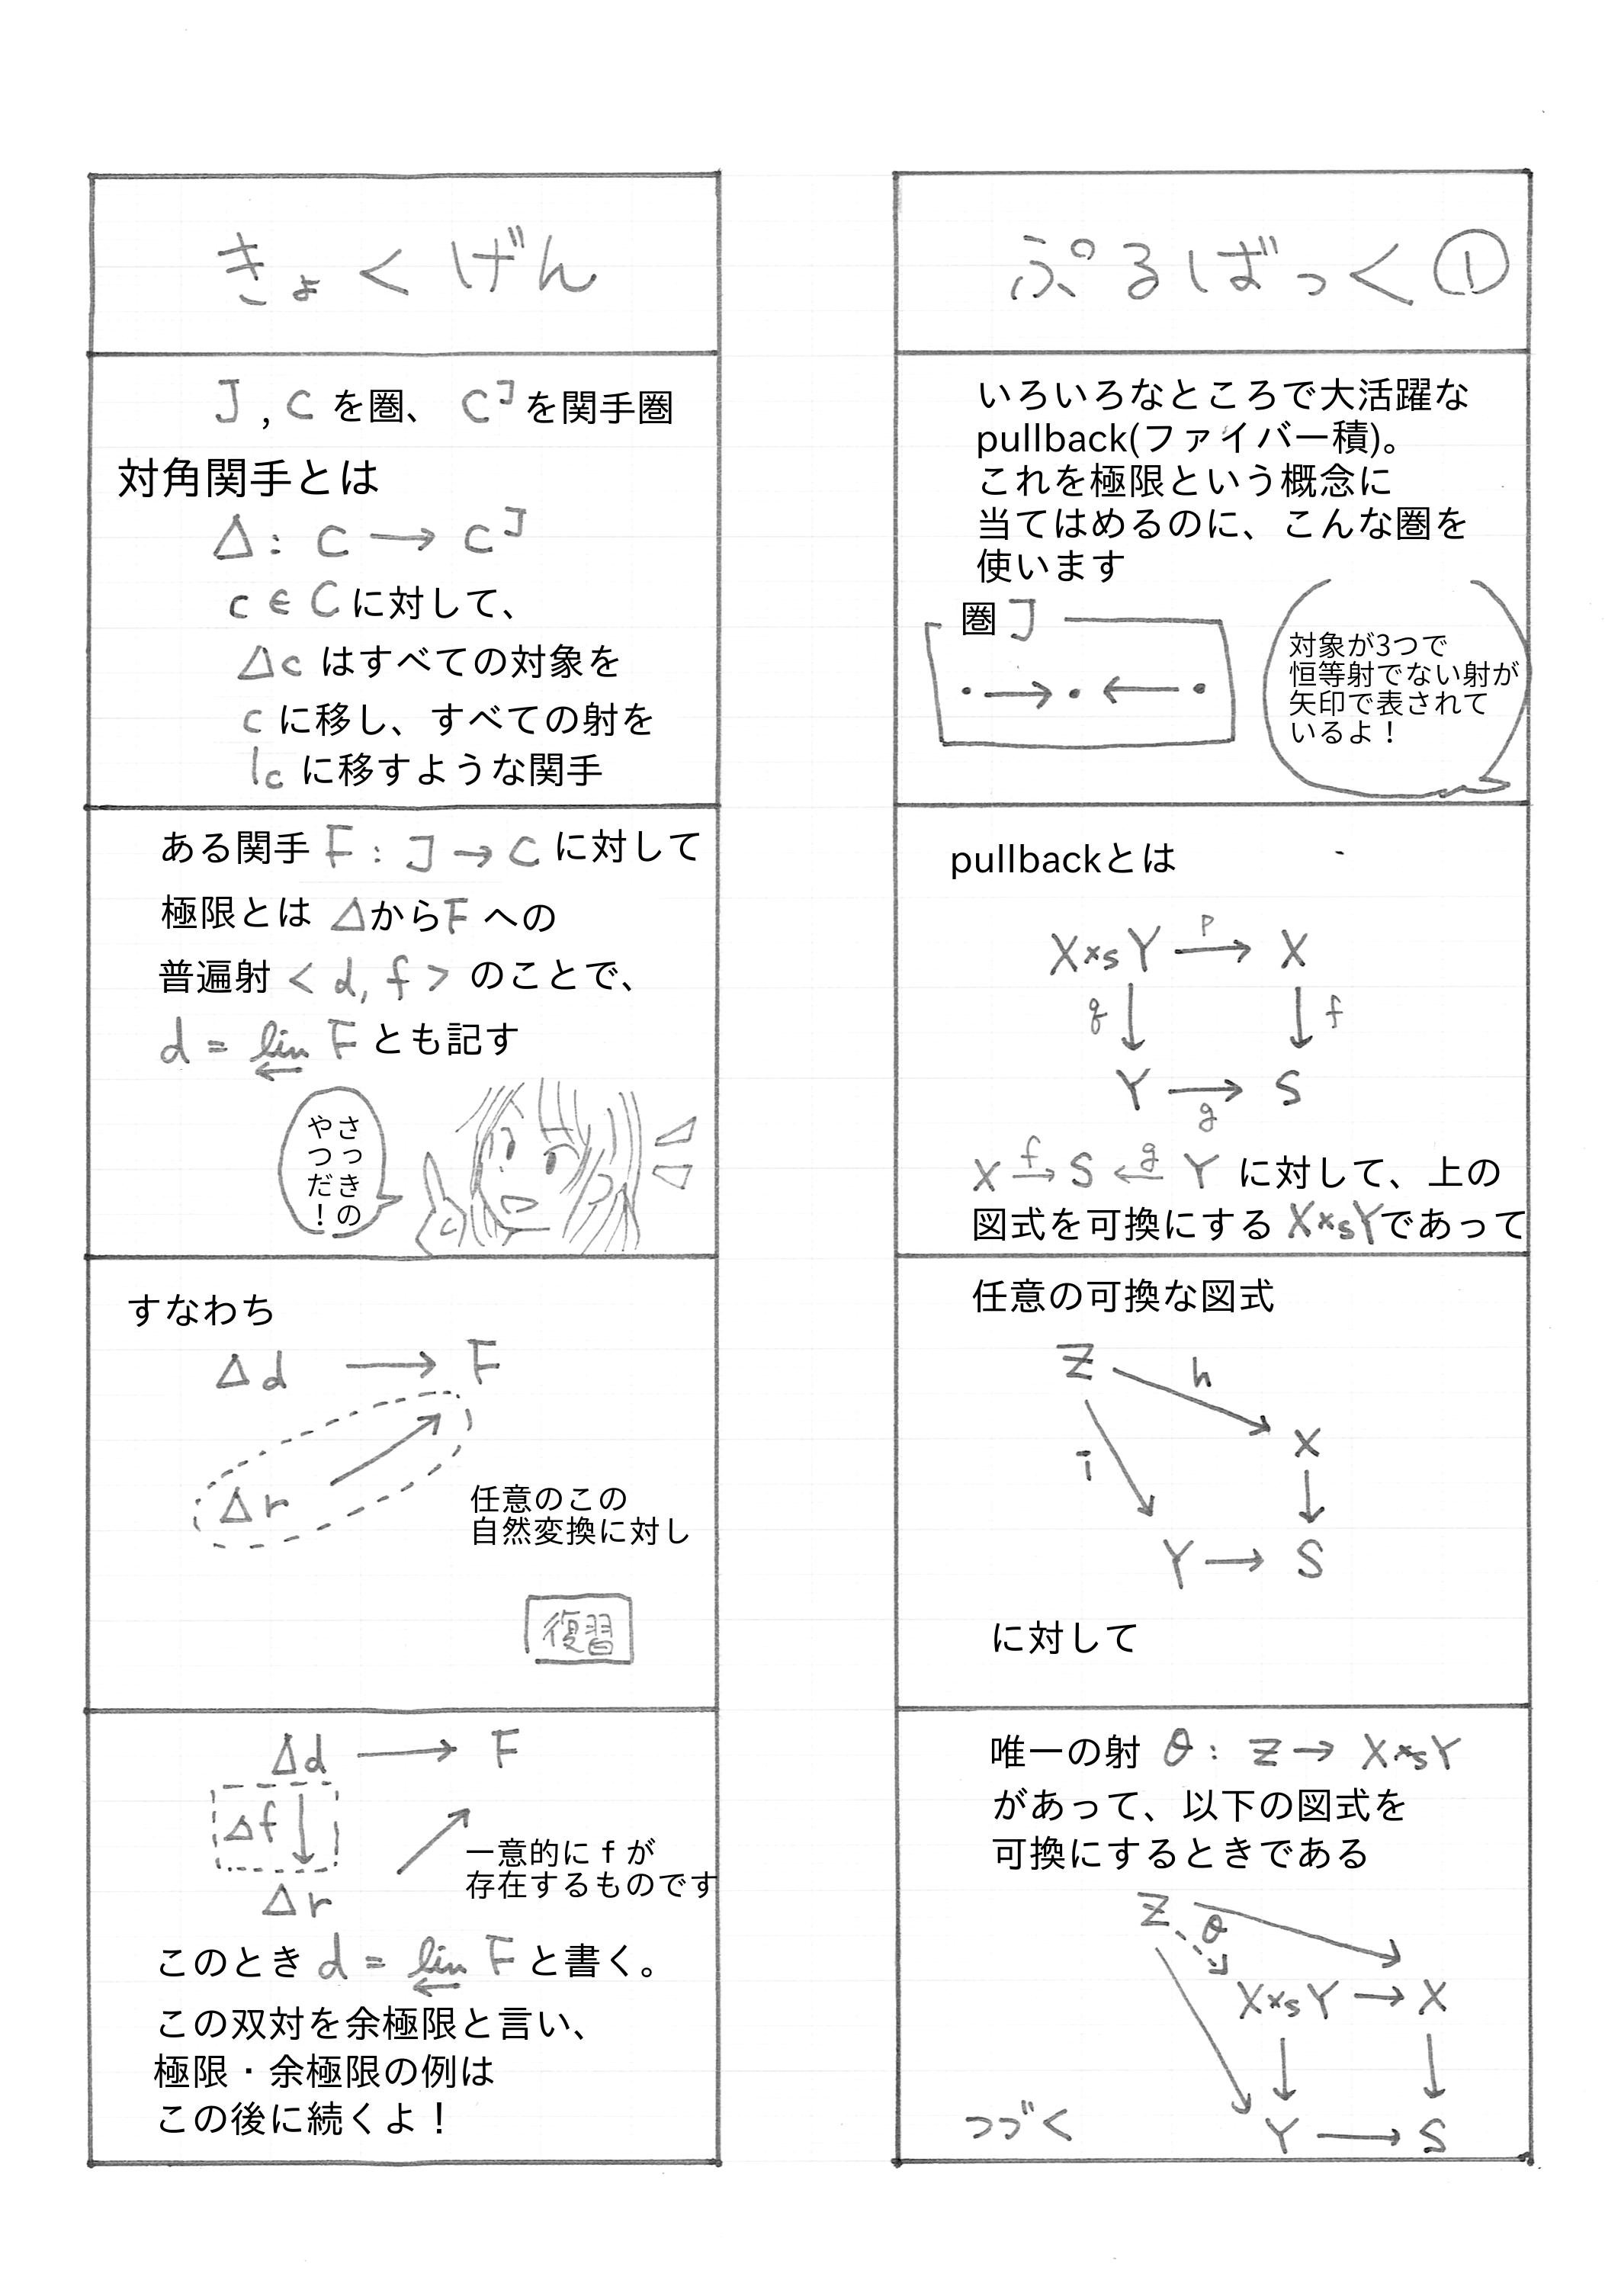
\includegraphics[width=13cm]{kobaken3.png}\\
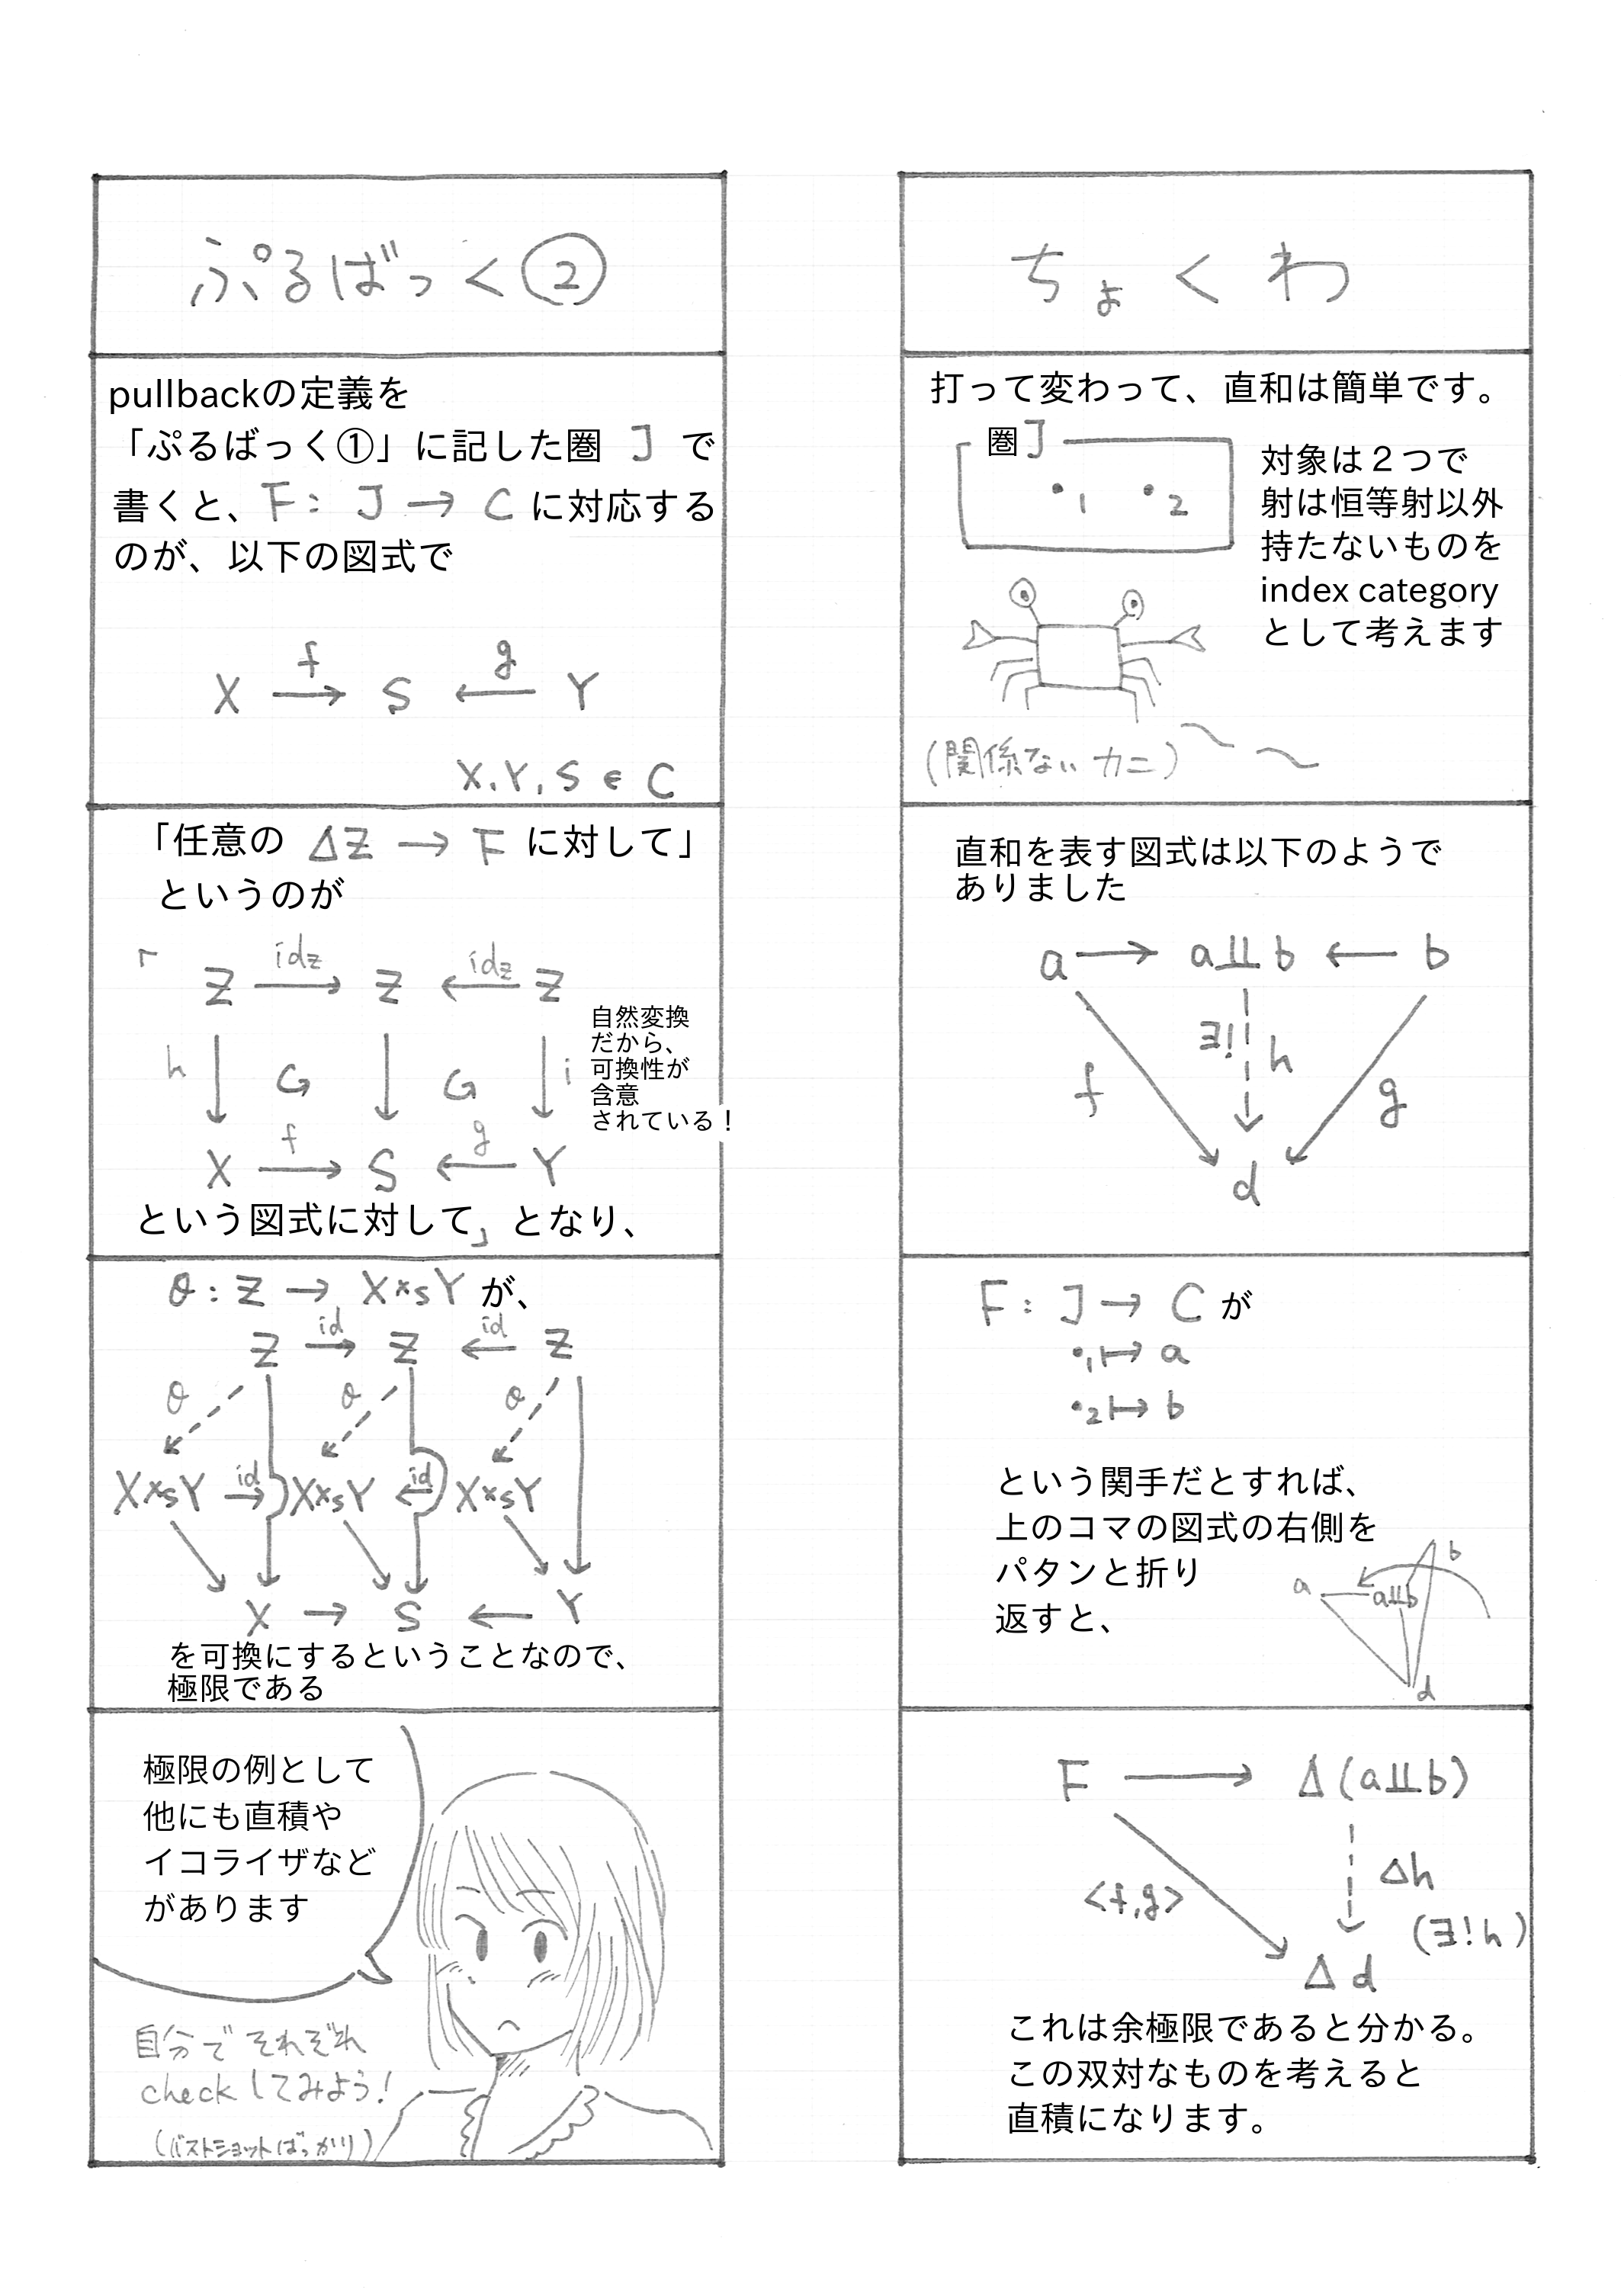
\includegraphics[width=13cm]{kobaken4.png}
%まず最初に使ったプリアンブルをここに書いてください.
%ただしコンパイルの都合上コメントアウトしてください.
%実際に確認する際は,各自の環境でmain.texにこのプリアンブルを追加してください.

%\usepackage{mathrsfs}
%\usepackage[all]{xy}
%\newcommand{\proofend}{\begin{flushright} $\blacksquare$ \end{flushright}}
%\renewcommand{\labelenumi}{(\roman{enumi})}
%\newcommand{\nkgr}{・}
%\theoremstyle{definition}
%\newtheorem{theorem}{定理}
%\renewcommand{\thetheorem}{}
%\newtheorem{ydefi}{定義}
%\newtheorem{ythm}[defi]{定理}
%\newtheorem{ylem}[defi]{補題}
%\newtheorem{ycor}[defi]{系}
%\newtheorem{yprop}[defi]{命題}
%\newtheorem{yex}[defi]{例}

\Chapter{Haar測度をつくろう(山本)}
\Section{\S 0. はじめに}
この項の目的を一言でいうと,「局所コンパクト位相群」の上で「良い振る舞い」をする「Haar測度」という測度を構成することです.
\Section{\S 1. もろもろの定義,お話}
有限群の表現論では,群$G$の元$s$を動かした際の総和を取って関数や内積を「平均化する」という手法があります.これをより一般の無限群でやろうとするわけですが,その際の「総和を取る」という操作は「積分」という形に置き換えればよさそうだということになります.積分を定めるためにはまず$G$上に測度を入れる必要がありますが,そのときに入れると便利な測度が,今回構成する「Haar測度」です.

Haar測度はそもそもとしてどのような測度なのかというと,数学的には次で定義されます.
\begin{ydefi}[Haar測度]\label{1}
局所コンパクト位相群$G$のBorel集合族$\mathscr{B}(G)$上の測度$\mu$が左不変Haar測度であるとは,次を満たすこと:
\begin{itemize}
 \item $G$のコンパクト集合$K$に対し,$\mu(K) < \infty$
 \item $G$の開集合$O$に対し,$\mu(O)=\sup \{ \mu(K) \mid K \subset O \colon \mathrm{compact} \}$
 \item $G$のBorel集合$B$に対し,$\mu(B)=\inf \{ \mu(O) \mid O \subset G \colon \mathrm{open} \}$
 \item Borel集合$B$および$s \in G$に対し,$\mu (B) = \mu (sB)$
\end{itemize}
$\mu$が右不変Haar測度であるとは,最後の条件を$\mu (B) = \mu (Bs)$に変えたものを満たすこと.
両側不変Haar測度とは,左かつ右不変Haar測度であること.
\end{ydefi}
Haar測度の良い点としては次の二つです:
\begin{itemize}
 \item $\mu$の定義域がBorel集合族$\mathscr{B}(G)$であるので,$G$の位相構造に対する振る舞いが良い.(正則性)
 \item 可測集合を左(右)移動しても,測度が変わらない.(左(右,両側)不変性)
\end{itemize}
これらの点において,非常に扱いやすい測度となっています.

Haar測度の例としては,
\begin{itemize}
 \item $\mathbb{R}^n$上のLebesgue測度
 \item 群に離散位相を入れたときの数え上げ測度
\end{itemize}
などがあります.2つ目において,特に有限群$G$に離散位相を入れたとき数え上げ測度を考えると,これによる$G$上の関数の積分は先に述べた「平均化」と一致することが分かります.

というわけで,今回示したいのは次の命題です.

\begin{yprop}[Haar測度の存在と一意性]\label{2}
局所コンパクト群$G$上には,左不変Haar測度が正の定数倍を除いて一意的に存在する.
\end{yprop}
この命題はFactとして用いられることが多いのですが,折角なので証明を追ってみようというのが本稿の目的です.今回の証明は,基本的にアンドレ・ヴェイユのつけた証明(参考文献[1])に依っています.

\Section{\S 2. 色々な準備}
この章では,各種理論から今回の証明に必要なものを(あまり証明はせずに)紹介します.

\Subsection{局所コンパクトHausdorff空間論からの準備}
まず,一般のコンパクト空間に関する主張です.

\begin{ythm}[Tychonoffの定理]\label{3}
$\{ K_i \} _{i \in I}$をコンパクト集合の族とするとき,$\prod_{i \in I} K_i$はコンパクト.
\end{ythm}
この証明は長いため省略します.例えば,参考文献[2]を参照してください.

\begin{ylem}\label{4}
$J$をコンパクト集合,$\{ F_i \}_{i \in I}$を$J$の閉集合の族とし,$\bigcap_{i \in I}F_i = \emptyset$とする.このとき,有限個の$F_{i_1}, \ldots , F_{i_n}$を選んで,$\bigcap_{j=1}^{n}F_{i_j} = \emptyset$とできる.
\end{ylem}
\begin{Proof}
$\bigcap_{i \in I}F_i = \emptyset$の両辺の補集合を取ると,$\bigcup_{i \in I}(F_i)^{c} = J$ すなわち,${(F_i)^{c}}_{i \in I}$は$J$の開被覆になります.$J$のコンパクト性から,有限個の$i_1, \ldots , i_n \in I$を選んで$\bigcup_{j=1}^{n}(F_{i_j})^{c} = J$とできます.再び両辺の補集合を取れば,$\bigcap_{j=1}^{n}F_{i_j} = \emptyset$となります.
\end{Proof}
続いて,局所コンパクトHausdorff空間について次のような主張があります.これらの証明も長いため,参考文献[3]に譲ります.
\begin{ythm}\label{5}
$X$を局所コンパクトHausdorff空間,$U \subset X \colon \mathrm{open}$,$K \subset U$をコンパクト集合とする.このとき,$V \subset X :\mathrm{compact}$であって,$K \subset \inter(V) \subset V \subset U$となるものが存在する.ただし,$\inter(V)$は$V$の$X$における内部とする.
\end{ythm}
\begin{ythm}[Urysohnの補題]\label{6}
$X$を局所コンパクトHausdorff空間,$U \subset X \colon \mathrm{open}$,$K \subset U \colon \mathrm{compact}$とする.このとき,次を満たす関数$f \colon X \to [0, 1]$が存在する:
\begin{itemize}
 \item $K$上$f \equiv 1$
 \item $X \setminus V$上$f \equiv 0$
\end{itemize}
\end{ythm}
\begin{ythm}[1の分割]\label{7}
$X$を局所コンパクトHausdorff空間,$K \subset X \colon \mathrm{compact}$,$\{ U_i \}_{i=1, \ldots , n}$を$K$の開被覆とする.このとき,次を満たす関数$f_i \colon X \to [0,1]$ $(i=1, \ldots , n)$が存在する:
\begin{itemize}
 \item $K$上$\sum_{i=1}^{n}h_i \equiv 1$
 \item 各$i=1, \ldots n$に対し,$\supp f_i \subset U_i$
\end{itemize}
\end{ythm}
続いて,今回の構成で決定的な役割をするRieszの表現定理について触れます.
\begin{ydefi}\label{8}
局所コンパクトHausdorff空間Xに対し, \\
 (1)$L_{+}(X)= \{ f \colon X \to \mathbb{R} \mid f \ge 0, \supp f \in X \colon \mathrm{compact}\}$ と定める. \\
 (2)$I \colon L_{+}(X) \to \mathbb{R}$が$L_{+}(X)$上の正の線形汎関数であるとは,次を満たすこと;
\begin{itemize}
 \item すべての$f \in L_{+}(X)$に対して,$I(f) \ge 0$
 \item すべての$f,g \in L_{+}(X)$に対して,$I(f+g)=I(f)+I(g)$
 \item すべての$f \in L_{+}(X), c \ge 0$に対して,$I(cf)=cI(f)$
\end{itemize}
\end{ydefi}
\begin{ythm}[Rieszの表現定理]\label{9}
$X$を局所コンパクトHausdorff空間,$I \colon X \to \mathbb{R}$を$L_{+}(X)$上の正の線形汎関数とする.このとき,$X$のBorel集合族$\mathscr{B}(X)$上の測度$\mu$であって,次を満たすものが存在する:
\begin{itemize}
 \item[(a)]すべての$f \in L_{+}(X)$に対して,$I(f)=\int_{X}fd\mu$
 \item[(b)]すべての$K \in X \colon \mathrm{compact}$に対して,$\mu(K)<\infty$
 \item[(c)]すべての$B \in \mathscr{B}(X)$に対して,$\mu(B)=\inf \{ \mu(O) \mid O \subset X \colon \mathrm{open} \}$
 \item[(d)]すべての$O \in X \colon \mathrm{open}$に対して,$\mu(O)=\sup \{ \mu(K) \mid K \subset O \colon \mathrm{compact} \}$
\end{itemize}
\end{ythm}
すなわち,$L_{+}(X)$上の正の線形汎関数に対して,$\mathscr{B}(X)$を定義域とする,いくつかの良い性質を持った測度が作れるということです.特に(b)(c)(d)を見ると,先の定義\ref{1}に出ていた性質そのものです.このことから,位相群$G$上のHaar測度を構成するためには,$L_{+}(X)$上の正の線形汎関数$I$であって,「左不変なもの」を構成してしまえばよさそうだということになります.実際,次のセクションからはその方向でHaar測度を構成していきます.

その際,「左不変性」を実際に証明するために必要な命題があります.

\begin{ylem}\label{10}
定理\ref{9}の状況で,$K$を$X$のコンパクト部分集合,$\chi_{K}$を$K$の特性関数とし,また$\varepsilon >0$とする.このとき,ある$g \in L_{+}(G)$が存在して,次を満たす:
\begin{itemize}
 \item $\mu ( \{ x \in X \mid \chi_{K}(x) \neq g(x) \} ) < \varepsilon $
 \item $g \le 1$
 \item $K$上$g \equiv 1$
\end{itemize}
\end{ylem}
\begin{Proof}
定理\ref{5}の$K$を$K$,$U$を$X$として適用すれば,$K \subset \inter(V) \subset V \subset X$となる$X$のコンパクト部分集合$V$が存在します.このとき,定理\ref{9}(c)を用いると,$n=1,2,\ldots$に対し,$K \subset V_n \subset V$なる$V_n \subset X \colon \mathrm{open}$で,$\mu(V_n) < \mu(K) + 2^{-n}\varepsilon$となるものが存在します.定理\ref{9}(b)から$\mu(K)<\infty$だったので,$\mu(V_n \setminus K) < 2^{-n}\varepsilon$となります.定理\ref{6}から,$f_n \colon X \to [0,1]$で,$f_n(X) \subset [0,1]$,$K$上$f_n \equiv 1$,$X \setminus V_n$上$f_n \equiv 0$なる$f_n$が存在します.$X \setminus V_{n}$上で$f_{n} \equiv 0$ですから,$\supp f_{n} \subset V$となり,$f_{n} \in L_{+}(G)$です.ここで,$g(x)=\sum_{n=1}^{\infty}2^{-n}f_n(x)$とおくと,$f_{n}(X) \subset [0,1]$からこの級数は一様収束なので,$g$は連続です.また,$\supp f_{n} \subset V$だったことから,$\supp g \subset V$も分かり,$g \in L_{+}(G)$となります.$f_n$は$K$上1なので,$g$も$K$上常に1です.$f_n \le 1$より$g \le 1$も分かります.最後に,$f_n$は$K$および$(V_n)^{c}$上では$\chi_{K}$と一致しているので,$\{ x \in X \mid \chi_{K}(x) \neq g(x) \} \subset \bigcup_{n=1}^{\infty}V_n \setminus K$です.したがって,$\mu( \{ x \in X \mid \chi_{K}(x) \neq g(x) \} ) \le \sum_{n=1}^{\infty} \mu(V_n \setminus K) < \sum_{n=1}^{\infty}2^{-n}\varepsilon=\varepsilon$となります.
\end{Proof}
\begin{yprop}\label{11}
定理\ref{9}の状況で,$\mu(K)= \inf \{ I(f) \mid f \in L_{+}(X), f|_{K} \equiv 1 \}$
\end{yprop}
\begin{Proof}
$K$上$f \equiv 1$なる$f \in L_{+}(G)$に対し,$ \mu(K)=\int_{X}\chi_K d\mu \le \int_{X}f d\mu=I(f)$より,$\mu(K) \le \inf \{ I(f) \mid f \in L_{+}(X), f|_{K} \equiv 1 \}$となります.逆の不等号を示すため,$\varepsilon>0$とします.補題10で,$\varepsilon$を$\varepsilon /2$として得られる$g$について,$U=\{ x \in X \mid \chi_{K}(x) \neq g(x) \}$とおくと$\| \chi_{K}-g\| _{L^1(X)} = \int_{X}|\chi_K-g|d\mu = \int_{U}(\chi_K-g)d\mu \le \int_{U}2 \cdot d\mu=2\mu(U)<2 \cdot \varepsilon / 2=\varepsilon$です.ゆえに$\| g\|  _{L^1(X)} < \| \chi_{K} \| _{L^1(X)} $ですが,これは$\chi_K, g \ge 0$から結局 $\int_{X}gd\mu < \int_{X}\chi_{K}d\mu +\varepsilon$,すなわち$I(g)<\mu (K)+\varepsilon$となります.$g$は$K$上で1でしたから,$\inf \{ I(f) \mid f \in L_{+}(X), f|_{K} \equiv 1 \} \le I(g) <\mu (K)+\varepsilon$となり,ここで$\varepsilon>0$は任意だったので,$\varepsilon \to 0$として $\inf \{ I(f) \mid f \in L_{+}(X), f|_{K} \equiv 1 \} \le \mu (K)$となります.
\end{Proof}
\Subsection{位相群論からの準備}

続いて,今回Haar測度を構成する舞台となる,位相群に関する準備です.

\begin{ydefi}[位相群]\label{12}
群演算の入ったHausdorff空間$G$が位相群であるとは,群の積演算:$G \times G \to G$および逆元を取る操作:$G \to G$がGの位相およびその積位相に関して連続であること.
\end{ydefi}
位相群の性質をいくつか見ておきます.
\begin{yprop}[位相群の性質]\label{13}
$G$を位相群とする.
\begin{itemize}
 \item[(1)]$G$の元$s$に関して,$s$を左(右)から掛ける操作:$G \to G$は同相写像である.
 \item[(2)]$G$の単位元$e$の近傍$U$に対し,ある$e$の近傍$V$が存在して,$VV \subset U$となる.ただし,$V,W \subset G$に対し,$VW= \{ vw \mid v \in V, w \in W \}$である.
\end{itemize}
\end{yprop}
\begin{Proof}
(1)同様なので,左から掛ける操作のときのみ示します.$s \in G$とすると,命題の写像は$G \to G \times G \to G ; g \mapsto (s,g) \mapsto sg$と,連続写像の合成として書けるので連続です.また,これには左から$s^{-1}$を掛けるという逆写像も存在し,これも連続なので結局与えられた写像は同相写像です.

(2)$U$を$e$の近傍とします.積位相の定義と積演算の連続性から,$e$の近傍$V_1, V_2$で,$v_{1} \in V_1, v_{2} \in V_2$なら$v_{1}v_{2} \in U$となるものが存在します.よって特に$V=V_1 \cap V_2$とすれば,これが欲しかった$e$の近傍になります.
\end{Proof}
後々の証明に必要なものを補題としていくつか作っておきます.

\begin{ylem}\label{14}
$G$のコンパクト部分集合$K$に対し,$K$上$f \equiv 1$となる$f \in L_{+}(G)$が取れる.
\end{ylem}
\begin{Proof}
定理\ref{5}の$K$を$K$,$U$を$G$として適用すれば,$K \subset \inter(V) \subset V \subset G$ となる$G$のコンパクト部分集合$V$が存在します.このとき,定理\ref{6}の$K$を$K$,$V$を$\inter(V)$として適用すれば,$K$上$f \equiv 1$および,$X \setminus \inter(V)$上$f \equiv 0$となる$f \colon X \to [0, 1]$が存在します.この$f$に対し,$x \in G$が$f(x)>0$を満たすなら$x \in \inter(V) \subset V$となりますから,$\supp f \subset V \colon \mathrm{compact}$となり,$f \in L_{+}(G)$となります.
\end{Proof}
\begin{ylem}\label{15}
$V$を$G$の単位元$e$の近傍とするとき,次を満たす$g \in L_{+}(G)$が取れる:
\begin{itemize}
 \item $g(e)>0$
 \item $G \setminus V$上$g(x)=0$
 \item すべての$x \in G$に対して,$g(x)=g(x^{-1})$
\end{itemize}
\end{ylem}
\begin{Proof}
逆元を取る操作の連続性から,$V^{-1}=\{ x^{-1} \mid x \in V \}$も$e$の近傍です.ゆえに$V \cap V^{-1}$も$e$の近傍です.定理\ref{5}の$K$を$\{e\}$に,$U$を$\inter(V \cap V^{-1})$として適用すると,$\{e\} \subset \inter(F) \subset F \subset V \cap V^{-1}$となる$G$のコンパクト部分集合$F$が存在します.このとき,$F^{-1}$も$e$のコンパクト近傍なので,$F \cap F^{-1}$も$e$のコンパクト近傍になります.定理\ref{6}を適用すると,$f(e)=1$,$\supp f \subset F \cap F^{-1}$となる$f \in L_{+}(G)$が存在します.$g(x)=f(x)+f(x^{-1})$なる$f' \in L_{+}(G)$を考えると,$g(e)=1+1=2>0$.また,すべての$x \in G$に対して,$g(x)=f(x)+f(x^{-1})=g(x^{-1})$です.そして,$\supp g \subset F \cap F^{-1} \subset V \cap V^{-1} \subset V$となるので,$G \setminus V$上$g(x)=0$となります. 
\end{Proof}

\begin{yprop}\label{16}
$G$:局所コンパクト位相群とするとき,$L_{+}(G)$の元は一様連続である.すなわち,任意の$\varepsilon>0$および$f \in L_{+}(G)$に対し,
\begin{itemize}
 \item $e$の近傍$V$であって,$xy^{-1} \in V_1$なる$x, y \in G$に対し,$|f(x)-f(y)|<\varepsilon$となるようなものが取れる.
 \item $e$の近傍$W$であって,$x^{-1}y \in V_1$なる$x, y \in G$に対し,$|f(x)-f(y)|<\varepsilon$となるようなものが取れる.
\end{itemize}
\end{yprop}
\begin{Proof}
同様なので,1つ目の場合のみ示します.$\varepsilon>0$とし,また$\supp f=K \colon \mathrm{compact}$とおきます.

まず,$e$の近傍$V_1$であって,$xy^{-1} \in V_1$なる$x \in G, y \in K$に対し,$|f(x)-f(y)|<\varepsilon$となるようなものが取れることを示します.$K$の元$a$に対し,$f$が連続であることから,ある$a$の近傍$V_a$が存在して,$f(V_a) \subset (f(a)-(\varepsilon /2), f(a)+(\varepsilon /2) )$となります.このとき,命題\ref{13}(1)から$V_{a}a^{-1}$は$e$の近傍なので,命題\ref{13}(2)により,$W_{a}W_{a} \subset V_{a}a^{-1}$となる$e$の近傍が取れます.このとき,$\bigcup_{a \in K}{W_a}a$は$K$の開被覆なので,$K$のコンパクト性から,有限個の$a_1, \ldots, a_n$を選んできて,$( W_{a_i}a_{i} )_{i=1,\ldots,n}$を$K$の部分被覆とできます.$V_1=\bigcap_{i=1}^{n}W_{a_i}$は$e$の近傍の有限個の共通部分なのでやはり$e$の近傍です.\\

この$V_1$が先に述べた条件を満たすことを示します.$x \in G, y \in K, xy^{-1} \in V_1$とします.$y \in K$より,ある$k \in \{1, \ldots , n \}$であって,$y \in W_{a_k}a_{k}$,すなわち$ya_{k}^{-1} \in W_{a_k} \subset V_{a_k}a_{k}^{-1}$となるものが存在します.このとき$y \in V_{a_k}$より$f(y) \in (f(a_k)-(\varepsilon/2), f(a_k)+(\varepsilon /2) )$ すなわち $|f(y)-f(a_k)|<\varepsilon /2$となります.さらに,$x(a_k)^{-1}=x(y^{-1})y(a_k)^{-1} \in VW_{a_k} \in W_{a_k}W_{a_k} \subset V_{a_k}a_{k}^{-1}$から,$|f(x)-f(a_k)|<\varepsilon /2$となります.よって,$|f(x)-f(y)|<\varepsilon$となることが分かりました.\\

同様にして,$e$の近傍$V_2$であって,$xy^{-1} \in V_1$なる$x \in K, y \in G$に対し,$|f(x)-f(y)|<\varepsilon$となるようなものが取れます.ここで,$V=V_1 \cap V_2$とおきます.これが命題の条件を満たす近傍になることを示します.$xy^{-1} \in V$とします.$x,y$の一方が$K$の元である場合は$xy^{-1} \in V_1 \cap V_2$より,先の場合に帰着できます.$x,y$の双方が$K=\supp f$の元でないときは,$f(x)=f(y)=0$となりますから,やはり$|f(x)-f(y)|=0<\varepsilon$が成り立ちます. 
\end{Proof}

これで,一通りの準備は終わりました.いよいよHaar測度を構成していきます.

\Section{\S 3. Haar測度の存在}
以降,$G$を局所コンパクト位相群とします.まず,構成だけでなく一意性の証明にも必要な道具を用意します.

\begin{ydefi}\label{17}
\leavevmode \\
(1)$s \in G, f \in L_{+}(G)$に対し,$Sf(x)=f(s^{-1}x)$として$Sf \in L_{+}(G)$を定める.\\
(2)$(\cdot : \cdot ) \colon L_{+}(G) \times L_{+}(G) \to [0, \infty) \cap \{ \infty \}$を次で定める:$f, g \in L_{+}(G)$とする.$G$の有限個の元$s_i$と,0以上の数$c_i$の組であって,すべての$x \in G$に対し$f(x) \le \sum_{i}c_{i} g(s_{i}^{-1}x)$となるものを考える.そのような組が存在するとき,$\sum_{i}c_i$の下限を$(f : g)$と定める.そのような組が存在しないとき,$(f : g)=\infty$と定める.
\end{ydefi}
今定義した写像の基本的な性質を見ておきます.
\begin{yprop}\label{18}
$f, g, h \in L_{+}(G)$とする.\\
(1)すべての$s \in G$に対し,$(Sf : g)=(f : g)$\\
(2)すべての$c \ge 0$に対し,$(cf : g)=c(f : g)$\\
(3)すべての$x \in G$に対し$f(x) \le g(x)$なら,$(f : h) \le (g : h)$\\
(4)$(f+g : h) \le (f : h)+(g : h)$\\
(5)$f \ne 0$なら,$( f : g ) > 0$\\
(6)$g \ne 0$なら,$( f : g ) < \infty $\\
(7)$h \ne 0$なら,$( f : g ) \le (f : g ) (g : h )$
\end{yprop}
\begin{Proof}
(1)〜(4)は定義に戻って考えれば分かります.

(5)$f \ne 0, f(x) \le \sum_{i}c_{i} g(s_{i}^{-1}x) (\forall x \in G)$とします.$g \in L_{+}(G)$より$g$は有界です.ゆえに,$f(x) \le \sum_{i}c_{i} g(s_{i}^{-1}x) \le \sum_{i}c_{i} \sup g$となり,$\sup f \le \sup g ( \sum_{i}c_{i} )$です.$c_i$たちに関する下限をとれば$0<\sup f \le \sup g (f : g )$となり,ここから(5)が従います.

(6)$g(s_{0}) > 0$なる$s_{0} \in G$を選び,$(1/2)g(s_{0})=m$とおきます.また,$C=\supp f \colon \mathrm{compact}$とおきます.$\Omega = g^{-1}( (m, \infty) )$とおくと$s_{0} \in \Omega \subset G \colon \mathrm{open}$で,$s \in G$に対して$s \in s s_{0}^{-1} \Omega \subset G \colon \mathrm{open}$です.族$( s s_{0}^{-1}\Omega )_{s \in G}$は$G$の開被覆であり,特に$C$の開被覆です.ゆえに,有限個の$ s_i(i=1,2, \ldots , n)$を選んで$( s_{i} s_{0}^{-1}\Omega )_{i=1,\ldots ,n}$が$C$の開被覆になるようにできます.$\sup f=M$とおくと,$x$に関する適当な場合分けにより$f(x) \le (M/m)\sum_{i} g( (s_{i} s^{-1}) ^{-1}x)$が分かります.ゆえに$(f : g ) \le nM/m < \infty $となります.

(7)は,$f \le \sum_{i} c_{i}S_{i}g, g \le \sum_{j} d_{j}T_{j}h$なら$f \le \sum_{i,j} c_{i}d_{j}S_iT_{j}h$となることが分かるので,$(f : h ) \le \sum_{i,j} c_{i}d_{j} = ( \sum_{i} c_{i} ) (\sum_{j} d_{j} )$から$( f : g ) \le (f : g ) (g : h )$となります. 
\end{Proof}

ここから,$L_{+}(G)$上の線形汎関数$I$を構成しにかかります.まず,値の「基準」となる$f_{0} \in L_{+}(G) \setminus \{ 0 \}$を一つ固定します.$G$の単位元$e$の近傍$V$全体を$\mathscr{V}$とおき,各$V \in \mathscr{V}$に対し,$G_{V}=\{ g \in L_{+}(G) \mid g(e)>0 かつ,全ての x \not\in V に対してg(x)=0 \}$と定めます.各$G_V$は補題\ref{15}により空ではありません.

\begin{yprop}\label{19}
$V \in \mathscr{V}, f \in L_{+}(G), g \in G_{V}$なら,
\[
0 \le \frac{1}{( f_0 : f )} \le \frac{( f : g )}{( f_0 : g )} \le ( f : f_0 ) < \infty
\]
である.ただし,$f=0$のとき$1/( f_0 : f ) = 0$と考える.
\end{yprop}
\begin{Proof}
$f=0$のとき,$( f : g ) = ( f : f_0 ) = 0$となるので特に命題は成り立ちます.
$f \ne 0$のとき,$g \neq 0$および命題\ref{18}の(7)から$(f_0 : g) \le (f_0 : f) (f : g )$,$ (f : g) \le (f : f_0 ) (f_0 : g )$が成り立ちます.$f, f_0 \neq 0$より,$(f_0 : g), (f_0 : f) \in (0, \infty)$が分かりますので,この不等式から主張が従います. 
\end{Proof}

各$f \in L_{+}(G)$に対し,$J_{f}=[1/ ( f_0 : f ) , ( f : f_{0} )]$と定めます.これは$\mathbb{R}$の有界閉区間なのでコンパクト集合です.そして,$J=\prod_{f \in L_{+}(G)} J_f$と定めます.これは定理\ref{3}によりコンパクト集合です.

また,$A \colon \bigcup_{V \in \mathscr{V}}G_V \to J$を,
\[
A(g)=\left( \frac{( f : g )}{( f_0 : g )} \right)_{f \in L_{+}(G)} \in J
\]
により定めます.$A$による$G_V$の像$A(G_V)$の$J$における閉包を$F_V$とおきます.
\begin{yprop}\label{20}
$\bigcap_{V \in \mathscr{V}}F_V \neq \emptyset$.
\end{yprop}
\begin{Proof}
背理法によります.左辺が空であるとすると,$J$がコンパクトだったので,補題4から$V_1, \ldots , V_n \in \mathscr{V}$で$\bigcap_{i=1}^{n}F_{V_i}=\emptyset$なるものが存在します.$V_0=\bigcap_{i=1}^{n}V_i$とおくと,これは$e$の近傍であり,$F_{V_0} \neq \emptyset$です.この元を1つとって$g$とおくと,$i=1, \ldots , n$に対し$g \in V_i$となるので,$A(g) \in \bigcap_{i=1}^{n}F_{V_i}=\emptyset$となり矛盾します. 
\end{Proof}

ゆえに,$I \in \bigcap_{V \in \mathscr{V}}F_V$なる$I$をとることができます.各$f \in L_{+}(G)$に対し,$I$の$J_f$成分を対応させる写像を$I \colon L_{+}(G) \to \mathbb{R}$と定めます.以降,これが線形汎関数となっていることを示しにいきます.
\begin{yprop}\label{21}
すべての$V \in \mathscr{V}$および有限個の$f_1, \ldots , f_n \in L_{+}(G)$,そして任意の$\varepsilon > 0$に対し,ある$g \in G_V$であって,$i=1, \ldots , n$に対し
\[
\lvert \frac{(f_i : g )}{( f_0 : g )} -I(f_i) \lvert < \varepsilon
\]
となるものが存在する.
\end{yprop}
\begin{Proof}
$i=1, \ldots , n$に対し,$U_i=J_{f_i} \cap ( I(f_i)- \varepsilon, I(f_i)+\varepsilon )$とおくと,$U_i$は$J_{f_i}$で開です.$J$の積位相を考えれば,$\prod_{f \neq f_1, \ldots , f_n}J_f \times U_1 \times \cdots \times U_n$は$J$で開です.この集合を$U$とおきます.$I(f_i) \in U_i$より,$I \in U$です.$I$は$F_V$,すなわち$A(G_V)$の閉包の元ですから,$A(G_V) \cap U \neq \emptyset$となります.$I' \in A(G_V) \cap U$を一つ取ると,ある$g \in G_V$が存在して,$I'=A(g)$です.このとき,$I' \in U$の$J_{f_i}$成分を見ると,$(f_i : g ) / ( f_0 : g ) \in U_i = ( I(f_i)- \varepsilon, I(f_i)+\varepsilon )$となります.よって$|(f_i : g ) / ( f_0 : g ) -I(f_i) | < \varepsilon$が成り立ちます.
\end{Proof}
命題\ref{21}を,より使いやすい形にしておきます.

\begin{ycor}\label{22}
$V_m \in \mathscr{V}(m \in \mathbb{N})$および有限個の$f_1, \ldots , f_n \in L_{+}(G)$に対し,$L_{+}(G)$の元の列$(g_m)_{m \in \mathbb{N}}$であって,各$m$に対して$g_m \in G_{V_m}$かつ,各$i=1, \ldots , n$に対して 
\[
\lim_{m \to \infty} \frac{(f_i : g_m )}{( f_0 : g_m )} =I(f_i)
\]
となるものが存在する.
\end{ycor}
\begin{Proof}
$m=1,2, \ldots$に対し,$g_m$を命題\ref{21}で$\varepsilon = 1/m$としたときの$g$として取ると,$|(f_i : g_m ) / ( f_0 : g_m ) -I(f_i) | < 1/m$となります.両辺の$m \to \infty$による極限を取れば, $\lim_{m \to \infty} (f_i : g_m ) / ( f_0 : g_m ) =I(f_i)$となります. 
\end{Proof}

\begin{yprop}\label{23}
$I$は$L_{+}(G)$上の正の線形汎関数である.すなわち,次が成り立つ. \\
(1)すべての$f \in L_{+}(X)$に対して,$I(f) \ge 0$\\
(2)すべての$f,g \in L_{+}(X)$に対して,$I(f+g)=I(f)+I(g)$\\
(3)すべての$f \in L_{+}(X), c \ge 0$に対して,$I(cf)=cI(f)$
\end{yprop}
\begin{Proof}
(1)は$I$の定義の仕方から明らかです.

(3)$V$を$e$の適当な近傍とします.系\ref{22}において,$m=1,2,\ldots$に対し$V_m=V$,$n=2$,$f_1=f$,$f_2=cf$としたときの$(g_m)_{m \in \mathbb{N}}$をとります.命題\ref{18}(2)より$(cf : g_m)=c(f : g_m)$で,両辺を$(f_0 : g_m)$で割って$m \to \infty$の極限をとれば,$I(cf)=cI(f)$となります.

(2)$V$を$e$の適当な近傍とし,系22において,$m=1,2,\ldots$に対し$V_m=V$,$n=3$,$f_3=f_1+f_2$としたときの$(g_m)_{m \in \mathbb{N}}$をとります.命題\ref{18}(4)より$(f_{1}+f_{2} : g_m ) \le (f_1 : g_m )+(f_1 : g_m)$となります.両辺を$(f_0 : g_m)$で割って$m \to \infty$の極限をとれば,$I(f_1+f_2) \le I(f_1)+I(f_2)$となります.
逆の不等号を示すため,次の補題を用意します.

\begin{ylem}\label{24}
$f, h, h'\in L_{+}(G)$とし,さらにすべての$x \in G$に対して$h(x)+h'(x) \le 1$とする.このとき,$I(fh)+I(fh') \le I(f)$.
\end{ylem}
\begin{Proof}
$m$を自然数とします.$h,h'$は命題\ref{16}により一様連続なので,ある$V_m \in \mathscr{V}$で,$s^{-1}x \in V_{m} \Rightarrow |h(x)-h(s)|, |h'(x)-h'(s)| \le 1/m$となるものが取れます.$V_m$をこの通りとし,$n=3, f_1=fh, f_2=fh', f_3=f$として系22のような$(g_m)_{m \in \mathbb{N}}$をとります.一旦$m$を一つに固定することとして,$f \le \sum_{i}c_i S_{i}g_m$となるような$c_i>0, s_i \in G$を考えます.$x \in G$に対し,$s_{i}^{-1}x \not\in V_m$なら$S_{i}g_{m}(x)=g_{m}(s_{i}^{-1}x)=0$です.ゆえに,$f(x) \le \sum_{s_{i}^{-1}x \in V_m} c_{i}S_{i}g_{m}(x)$です.$s_{i}^{-1}x \in V_m$であるとき,$|h(x)-h(s_i)| \le 1/m$より,$h(x) \le h(s_i)+(1/m)$で,
\begin{align*}
f(x)h(x)  & \le \sum_{s_{i}^{-1}x \in V_m} c_{i}S_{i}g_{m}(x)h(x) \\
& \le \sum_{s_{i}^{-1}x \in V_m} c_{i}S_{i}g_{m}(x) \left( h(s_i)+\frac{1}{m} \right) \\
& \le \sum_{i}c_{i} \left( h(s_i)+\frac{1}{m} \right) S_{i}g_{m}(x) \\
\end{align*}
となります.よって,$( fh : g_m ) \le \sum_{i}c_{i} ( h(s_i)+(1/m) )$ です.$h'$も同様に,$( fh' : g_m ) \le \sum_{i}c_{i} ( h'(s_i)+(1/m) )$ です.これら2式を足して,
\[
( fh : g_m )+( fh' : g_m ) \le \sum_{i}c_{i} \left( h(s_i)+h'(s_i)+\frac{2}{m} \right) \le \sum_{i}c_{i} \left( 1+\frac{2}{m} \right)
\]
となります.$\sum_{i}c_{i}$ に関する下限をとって,$( fh : g_m )+( fh' : g_m ) \le ( f : g_m ) ( 1+(2/m) )$です.両辺を$(f_0 : g_m)$で割って$m \to \infty$の極限をとれば,$I(fh)+I(fh') \le I(f)$となります. 
\end{Proof}
命題\ref{23}の証明に戻ります.$\supp (f_{1}+f_{2})=C$とおきます.$f_1, f_2 \ge 0$より,$\supp f_1, \supp f_2 \subset C$です.補題14により,$C$上常に1となる$f' \in L_{+}(G)$がとれます.$\varepsilon>0$とし,$F_{\varepsilon}=f_{1}+f_{2}+\varepsilon f'$とおきます.$h,h' \in L_{+}(G)$を次で定めます:
\[
h(x)=
\begin{cases}
f_{1}(x)/F_{\varepsilon}(x) & (x \in C) \\
0 & (x \not\in C)
\end{cases}
\]
\[
h'(x)=
\begin{cases}
f_{2}(x)/F_{\varepsilon}(x) & (x \in C) \\
0 & (x \not\in C)
\end{cases}
\]
$x \in C$かどうかで場合分けすれば,$f_{1}=hF_{\varepsilon}, f_{2}=h'F_{\varepsilon}, h+h' \le 1$が分かります.よって,補題24から
\begin{align*}
I(f_1)+I(f_2) = I(hF_{\varepsilon})+I(h'F_{\varepsilon}) & \le I(F_{\varepsilon})=I ( (f_{1}+f_{2})+\varepsilon f' ) \\
& \le I(f_{1}+f_{2})+ \varepsilon I(f')
\end{align*}
となります.$\varepsilon$は任意だったので,$\varepsilon \to 0$として,$I(f_1)+I(f_2) \le I(f_{1}+f_{2})$が従います.以上により,$I(f+g)=I(f)+I(g)$が言えました. 
\end{Proof}

命題\ref{23}により,$I$が正の線形汎関数であることが分かりました.したがって定理\ref{9}により,$I$に対応する測度$\mu$ができます.残すは左不変性のみとなりました.

\begin{yprop}\label{25}
すべての$B \in \mathscr{B}(G), s \in G$に対し,$sB \in \mathscr{B}(G)$であって,$\mu(sB)=\mu(B)$である.すなわち,$\mu$は$G$上のHaar測度である.
\end{yprop}
\begin{Proof}
まず,命題\ref{18}(1)を用いれば,命題\ref{23}(3)と同じ方法により$I(f)=I(Sf)$が従います.これを踏まえ,3つのステップに分けて証明を行います.

(Step1)$K \in G \colon \mathrm{compact}$のとき.

$sK \subset G \colon closed$より,$sK \in  \mathscr{B}(G)$です.
\begin{align*}
\mu(K) & = \inf \{ I(f) \mid f \in L_{+}(X), f|_{K} \equiv 1 \} \\
 & =\inf \{ I(f) \mid f \in L_{+}(X), f|_{sK} \equiv 1 \}=\mu(sK)
\end{align*}
となります.ただし,1つ目と3つ目の等号は命題\ref{11}から従います.2つ目の等号は,$\{ f \in L_{+}(X) | f|_{K} \equiv 1 \}$と$\{ f \in L_{+}(X) | f|_{sK} \equiv 1 \}$の間に$f \mapsto Sf$という1対1対応があり,この対応に関して$I(f)=I(Sf)$が成り立っていたことから分かります

(Step2)$O \in G \colon \mathrm{open}$のとき.

$sO \subset G \colon \mathrm{open}$より,$sO \in \mathscr{B}(G)$です.
\begin{align*}
\mu(O) & = \sup \{ \mu(K) \mid K \subset O \colon \mathrm{compact} \} \\
 & =\sup \{ \mu(K) \mid K \subset sO \colon \mathrm{compact} \} = \mu (O)
\end{align*}
となります.ただし,1つ目と3つ目の等号は定理\ref{9}の性質(d),2つ目の等号は,$\{ K \subset O \mid \mathrm{compact} \}$と$\{ K \subset sO \mid \mathrm{compact} \}$との間に$K \mapsto sK$という1対1対応があり,この対応に関して(Step1)から$\mu(K)=\mu(sK)$が成り立っていたことから分かります.

(Step3)$B \in \mathscr{B}(G)$のとき.

$\mathscr{M}=\{A \in \mathscr{B}(G) \mid \forall s \in G , sB \in \mathscr{B}(G) \}$とおくと,これは単調族であって,(Step2)から$G$の開集合を全て元に持ちます.よって,$\mathscr{M}$は$G$の全ての開集合を元に持つ最小の完全加法族,すなわちBorel集合族を含みます.これは$B \in \mathscr{B}(G), s \in G$に対し$ sB \in \mathscr{B}(G)$が成り立つことを意味しています.そして,
\begin{align*}
\mu(B) & = \inf \{ \mu(O) \mid B \subset O \subset G \colon \mathrm{open}\} \\
 & = \inf \{ \mu(O) \mid sB \subset O \subset G \colon \mathrm{open}\} = \mu(sB)
\end{align*}
となります.ただし,1つ目と3つ目の等号は定理\ref{9}の性質(c),2つ目の等号は,$\{ O \subset G \mid \mathrm{open}, B \subset O \}$と$\{ O \subset G \mid \mathrm{open}, sB \subset O \}$との間に$O \mapsto sO$という1対1対応があり,この対応に関して(Step2)から$\mu(O)=\mu(sO)$が成り立っていたことから分かります.

以上により,Borel集合族の元である集合の測度は左移動で不変であることが分かり,$\mu$が左不変Haar測度であることが示されました. 
\end{Proof}
\Section{\S 4. Haar測度の一意性}
先のセクションで,(左不変)Haar測度の存在が示されました.このセクションではさらに,Haar測度の一意性を示していきます.

\begin{yprop}\label{26}
$G$を局所コンパクト位相群とし,$\mu_1, \mu_2$を$G$上の左不変Haar測度とする.このとき,ある$c>0$が存在して,すべての$B \in \mathscr{B}(G)$に対して,$\mu_1(B)=c\mu_2(B)$が成り立つ.すなわち,左不変Haar測度は正の定数倍を除いて一意である.
\end{yprop}
この命題を示すためには,次の命題を示せば十分です.
\begin{yprop}\label{27}
$\mu$を局所コンパクト位相群$G$上の左不変Haar測度とし,$I \colon L_{+}(G) \to \mathbb{R}$を,$I(f)=\int_{G}f d\mu$により定める.$f_0 \in L_{+}(G)$を固定すると,$I(f)/I(f_0)$の値は左不変Haar測度の値によらない.
\end{yprop}
まず,命題\ref{27}が示されたとして,命題\ref{26}が成立することを示します.
\begin{Proof}(命題\ref{27}$\Rightarrow$命題\ref{26}) $\mu_1, \mu_2$を$G$の左不変Haar測度とし,対応する積分を$I_1, I_2$とおくと,命題\ref{27}から,すべての$f \in L_{+}(G)$に対して$I_{1}(f)/I_{1}(f_0)=I_{2}(f)/I_{2}(f_0)$となるので,$I_{1}(f)= \left( I_{1}(f_0)/I_{2}(f_{0}) \right) I_{2}(f)$が成り立ちます.そこで$c=\left( I_{1}(f_0)/I_{2}(f_{0}) \right)(>0)$とおくと,すべての$f \in L_{+}(G)$に対して$I_{1}(f)= c I_{2}(f)$が成り立ちます.あとは命題25と同じようにやれば命題\ref{26}が従います.
\end{Proof}

それでは,命題\ref{27}の証明に入ります.
\begin{Proof}(命題\ref{27})
$f \in L_{+}(G)$とします.$f=0$のときは$I(f)=0$となるので,$f \neq 0$としてよいことが分かります.$C=\supp f \cup \supp f_{0}$とおきます.この$C$は定め方からコンパクトです.また,後で使うのですが,$C$上$f' \equiv 1$となるような$f' \in L_{
+}(G)$を1つ取ります.これは補題14から取れることが分かっています.$f, f' \neq 0$より,$\left( f' : f\right)$は0でも$\infty$でもありません.そこで,$m=1,2,\ldots$に対し,$\varepsilon_{m}=\frac{1}{(m+1)\left( f' : f \right)}>0$と置きます.$f$は命題\ref{16}から一様連続なので,$m=1,2,\ldots$に対してある$V_m \in \mathscr{V}$が存在して,$s^{-1}x \in V_m$なら$|f(x)-f(s)|<\varepsilon _{m}$となるようにできます.各$V_m$に対し,補題15のような$g_m$を1つずつ取ります.以降しばらく,$m$を1つ固定して考えます.

積分 $\int_{G}f(s)g_{m}(s^{-1}x)d\mu(s)$を考えます.$s^{-1}x \not\in V_m$なら$g_{m}(s^{-1}x)=0$,$s^{-1}x \in V_m$なら$f(s) \ge f(x) -\varepsilon_{m}$であることから,
\begin{align*}
\int_{G}f(s)g_{m}(s^{-1}x)\mu(s) & =\int_{Vx^{-1}}f(s)g_{m}(s^{-1}x)\mu(s) \\
 & \ge (f(x)-\varepsilon_{m})\int_{Vx^{-1}}g_{m}(s^{-1}x)\mu(s) \\
 & =(f(x)-\varepsilon_{m})\int_{Vx^{-1}}g_{m}(s^{-1}x)\mu(s)
\end{align*}
となりますが,$g_{m}$の取り方から$g_{m}(s^{-1}x)=g_{m}\left( (s^{-1}x)^{-1} \right)=g_{m}(x^{-1}s)$となるので,上式は
\begin{align*}
\int_{G}f(s)g_{m}(s^{-1}x)d\mu(s) & \ge (f(x)-\varepsilon_{m})\int_{Vx^{-1}}g_{m}(s^{-1}x)\mu(s) \\
 & = (f(x)-\varepsilon_{m})\int_{Vx^{-1}}g_{m}(x^{-1}s)\mu(s) \\
 & =(f(x)-\varepsilon_{m}) I(g_{m})
\end{align*}
となります.ゆえに,
\begin{equation}
(f(x)-\varepsilon_{m}) \le \left( 1/I(g_{m}) \right)\int_{G}f(s)g_{m}(s^{-1}x)d\mu(s)
\label{i2}
\end{equation}
であることが分かります.

ここで,$g_{m} \in L_{+}(G)$より,再び命題\ref{16}から,任意の$\eta >0$に対し,ある$W \in \mathscr{V}$であって,$yz^{-1} \in W$なら$|g_{m}(y)-g_{m}(z)|<\eta$となるものがあります.

さらに,$G$の有限個の元$s_{i}$および関数$h_i \in L_{+}(G)$で,$C$上$\sum_{i}h_i \equiv 1$となり,さらに各$h_i$が$G \setminus s_{i}W$上で0になるようなものを取ることができます(ディユドネ分割):実際,$(sW)_{s \in G}$は$G$の開被覆なので特に$C$の開被覆で,$C$のコンパクト性より有限個の$s_i \in G$を取って,$(s_{i}W)_{i}$が有限部分被覆となるようにできます.これに対応する1の分割(定理\ref{7})により,この分割の存在が言えます.このとき,
\begin{align*}
\int_{G}f(s)g_{m}(s^{-1}x)d\mu(s) & =\int_{C}1 \cdot f(s)g_{m}(s^{-1}x)d\mu(s) \\
 & =\int_{C} \left( \sum_{i}h_{i}(s) \right) f(s)g_{m}(s^{-1}x)d\mu(s) \\
 & =\sum_{i} \int_{C}h_{i}(s)f(s)g_{m}(s^{-1}x)d\mu(s) \\
 & =\sum_{i} \int_{G}h_{i}(s)f(s)g_{m}(s^{-1}x)d\mu(s)
\end{align*}
です.$s \not\in s_{i}W$なら$h_{i}(s)=0$であり,一方$s \in s_{i}W$なら$s_{i}^{-1}x(s^{-1}x)^{-1}=s_{i}^{-1}s \in W$であることから$g_{m}(s^{-1}x) \le g_{m}(s_{i}^{-1}x) + \eta$となります.よって, 
\begin{align*}
\int_{G}h_{i}(s)f(s)g_{m}(s^{-1}x)d\mu(s) & =\int_{s_{i}W}h_{i}(s)f(s)g_{m}(s^{-1}x)d\mu(s) \\
 & \le \int_{s_{i}W}h_{i}(s)f(s)\left( g_{m}(s_{i}^{-1}x) + \eta \right) d\mu(s) \\
 & =\left( g_{m}(s_{i}^{-1}x) + \eta \right) \int_{G}h_{i}(s)f(s)d\mu(s) \\
 & =\left( g_{m}(s_{i}^{-1}x) + \eta \right)I(fh_{i})
\end{align*}
となります.ゆえに,先の等式と合わせて
\begin{equation}
\int_{G}f(s)g_{m}(s^{-1}x)d\mu(s) \le \sum_{i}\left( g_{m}(s_{i}^{-1}x) + \eta \right)I(fh_{i}) 
\label{i1}
\end{equation}
が分かります.

$c_i=I(fh_i)/I(g_{m})$とおくと,
\begin{align*}
\sum_{i}c_{i}=\sum_{i}s_{i}  \frac{1}{I(g_{m})} \int_{G}f(x)h_{i}(x)d\mu & = \frac{1}{I(g_{m})}\int_{C}f(x) \left( \sum_{i}s_{i}h_{i}(x) \right) d\mu \\
 & =\frac{1}{I(g_{m})}\int_{C}f(x) d\mu \\
 & =\frac{1}{I(g_{m})}\int_{G}f(x) d\mu=\frac{I(f)}{I(g_{m})}
\end{align*}
であって,不等式(\ref{i2}),(\ref{i1})から
\begin{align*}
f(x)-\varepsilon_{m} & \le \frac{1}{I(g_{m})} \int_{G}f(s)g_{m}(s^{-1}x)d\mu(s) \\ 
 & \le \frac{1}{I(g_{m})} \sum_{i}\left( g_{m}(s_{i}^{-1}x) + \eta \right)I(fh_{i})
\end{align*}
が分かるので,これを整理して$f(x) \le \varepsilon_{m} + \eta \sum_{i}c_{i} + \sum_{i}c_{i}S_{i}g_{m}(x)$が分かります.ここでさらに,
\begin{equation}
f(x) \le \left( \varepsilon_{m} + \eta \sum_{i}c_{i} \right)f'(x) + \sum_{i}c_{i}S_{i}g_{m}(x)
\label{i3}
\end{equation}
とできます.($x \in C$かどうかで場合分けすれば分かります.) また,$\sum_{i}c_{i}S_{i}g_{m}(x) \le \sum_{i}c_{i}S_{i}g_{m}(x)$より, $\left( \sum_{i}c_{i}S_{i}g(x) : g_{m} \right) \le \sum_{i}c_{i}=I(f)/I(g)$です.以上を踏まえて,(\ref{i3})の両辺を$\left( \cdot : g_{m} \right) $の$\cdot$に代入すると,命題\ref{18}(2)(3)(4)から 
\begin{align*}
\left( f : g_{m} \right) & \le \left( \left( \varepsilon_{m} + \eta \sum_{i}c_{i} \right)f' +  \sum_{i}c_{i}S_{i}g_{m} : g_{m} \right) \\
 & \le \left( \varepsilon_{m} + \eta \sum_{i}c_{i} \right) \left( f' : g_{m} \right) + \left( \sum_{i}c_{i}S_{i}g_{m}(x) : g_{m} \right) \\
 & \le \left( \varepsilon_{m} + \eta \sum_{i}c_{i} \right) \left( f' : g_{m} \right) + \frac{I(f)}{I(g_{m})}
\end{align*}
となります.$\eta>0$は任意だったので,$\eta \to +0$として,
\begin{equation}
\left( f : g_{m} \right) \le \varepsilon_{m} \left( f' : g_{m} \right) + \frac{I(f)}{I(g_{m})}
\label{i4}
\end{equation}
が分かります.

この(\ref{i4})に関して,さらに命題\ref{18}(7)から$\left( f : g_{m} \right) \le \varepsilon_{m} \left( f' : f \right) \left( f : g_{m} \right) + I(f)/I(g_{m})$です.ゆえに$\varepsilon_{m}$の定義を思い出しつつ整理すると $\left( m/(m+1) \right) \left( f : g_{m} \right)I(g_{m}) \le I(f)$,$\left( f : g_{m} \right)I(g_{m}) \le I(f)(m+1)/m \le 2I(f)$となります.よって,$ \left( f' : g_{m} \right)I(g_{m}) \le 
\left( f' : f \right) \left( f : g_{m} \right) I(g_{m}) \le 2I(f)\left( f' : f \right)$となります.ここまでをまとめると
\begin{equation}
0<\frac{I(f)}{I(g_{m})} \le \left( f : g_{m} \right) \le \varepsilon_{m} \left( f' : f \right) \left( f : g_{m} \right) + \frac{I(f)}{I(g_{m})}
\label{i5}
\end{equation}
です.さて,ここまでの議論をよくみると,$f_0$に対しても全く同様な議論が行えることが分かります.すなわち,
\begin{equation}
0<\frac{I(f_0)}{I(g_{m})} \le \left( f_0 : g_{m} \right) \le \varepsilon_{m} \left( f' : f_0 \right) \left( f_0 : g_{m} \right) +\frac{I(f_0)}{I(g_{m})}
\label{i6}
\end{equation}
が成り立ちます.(\ref{i6})の辺々の逆数を取り,(\ref{i5})に辺々掛けて整理すると
\begin{equation}
\frac{I(f)}{\varepsilon_{m} \left( f' : g_{m} \right)I(g_{m}) + I(f_0)} \le \frac{(f : g_{m}) }{(f_0 : g_{m})} \le \frac{ \varepsilon_{m} \left( f' : g_{m} \right)I(g_{m}) + I(f) }{I(f_0)}
\label{i7}
\end{equation}
となります.

$\lim_{m \to \infty}\varepsilon_{m} =0, \sup_{m \in \mathbb{N}}\left( f' : g_{m} \right)I(g_{m}) \le 2I(f)\left( f' : f \right) < \infty$より,
\[
\lim_{m \to \infty}\varepsilon_{m} \left( f' : g_{m} \right)I(g_{m})=0
\]
となります.これを踏まえて(\ref{i7})の辺々の$m \to \infty$における極限を取って,
\[
\frac{I(f)}{I(f_{0})} \le \lim_{m \to \infty} \frac{\left(f : g_{m} \right)}{\left( f_{0} : g_{m} \right)} \le \frac{I(f)}{I(f_{0})}
\]
すなわち $I(f)/I(f_{0})=\lim_{m \to \infty} \left( f : g_{m} \right) / \left( f_{0} : g_{m} \right)$となります.この式の右辺において,$g_{m}$の構成は$f, f_{0}$のみに依っていたので,その値はHaar測度によりません.したがって左辺もHaar測度によらないことが分かり,これによってHaar測度の一意性が示されました. 
\end{Proof}

\Section{\S 5. おわりに}
今回は局所コンパクト位相群のHaar測度の存在および一意性を証明しました.この記事の執筆を通して,有名な事実の証明を1つキチンと追うのは結構大変だということを痛感しました.ある意味修行のような記事になったと感じておりますが,それはそれでよい経験になったとも思います.この記事を通して,何か皆さんに伝わるものがあれば幸いです.最後に,実際に証明を追うにあたって,参考文献の紹介や,証明を実際にいくつか付けてくれた友人に感謝の意を述べ,この記事を閉じさせていただきます.

\begin{thebibliography}{9}
\item アンドレ・ヴェイユ 齋藤正彦訳『位相群上の積分とその応用』,ちくま学芸文庫
\item 内田伏一『集合と位相』,裳華房
\item W. Rudin,Real and Complex Analysis, 3rd ed., McGraw-Hill Book Company
\item ポントリャーギン 柴岡泰光,杉浦光夫,宮崎功訳『連続群論 上』,岩波書店
\end{thebibliography}

\Section{圏論が分かる4コマ漫画4(小林)}
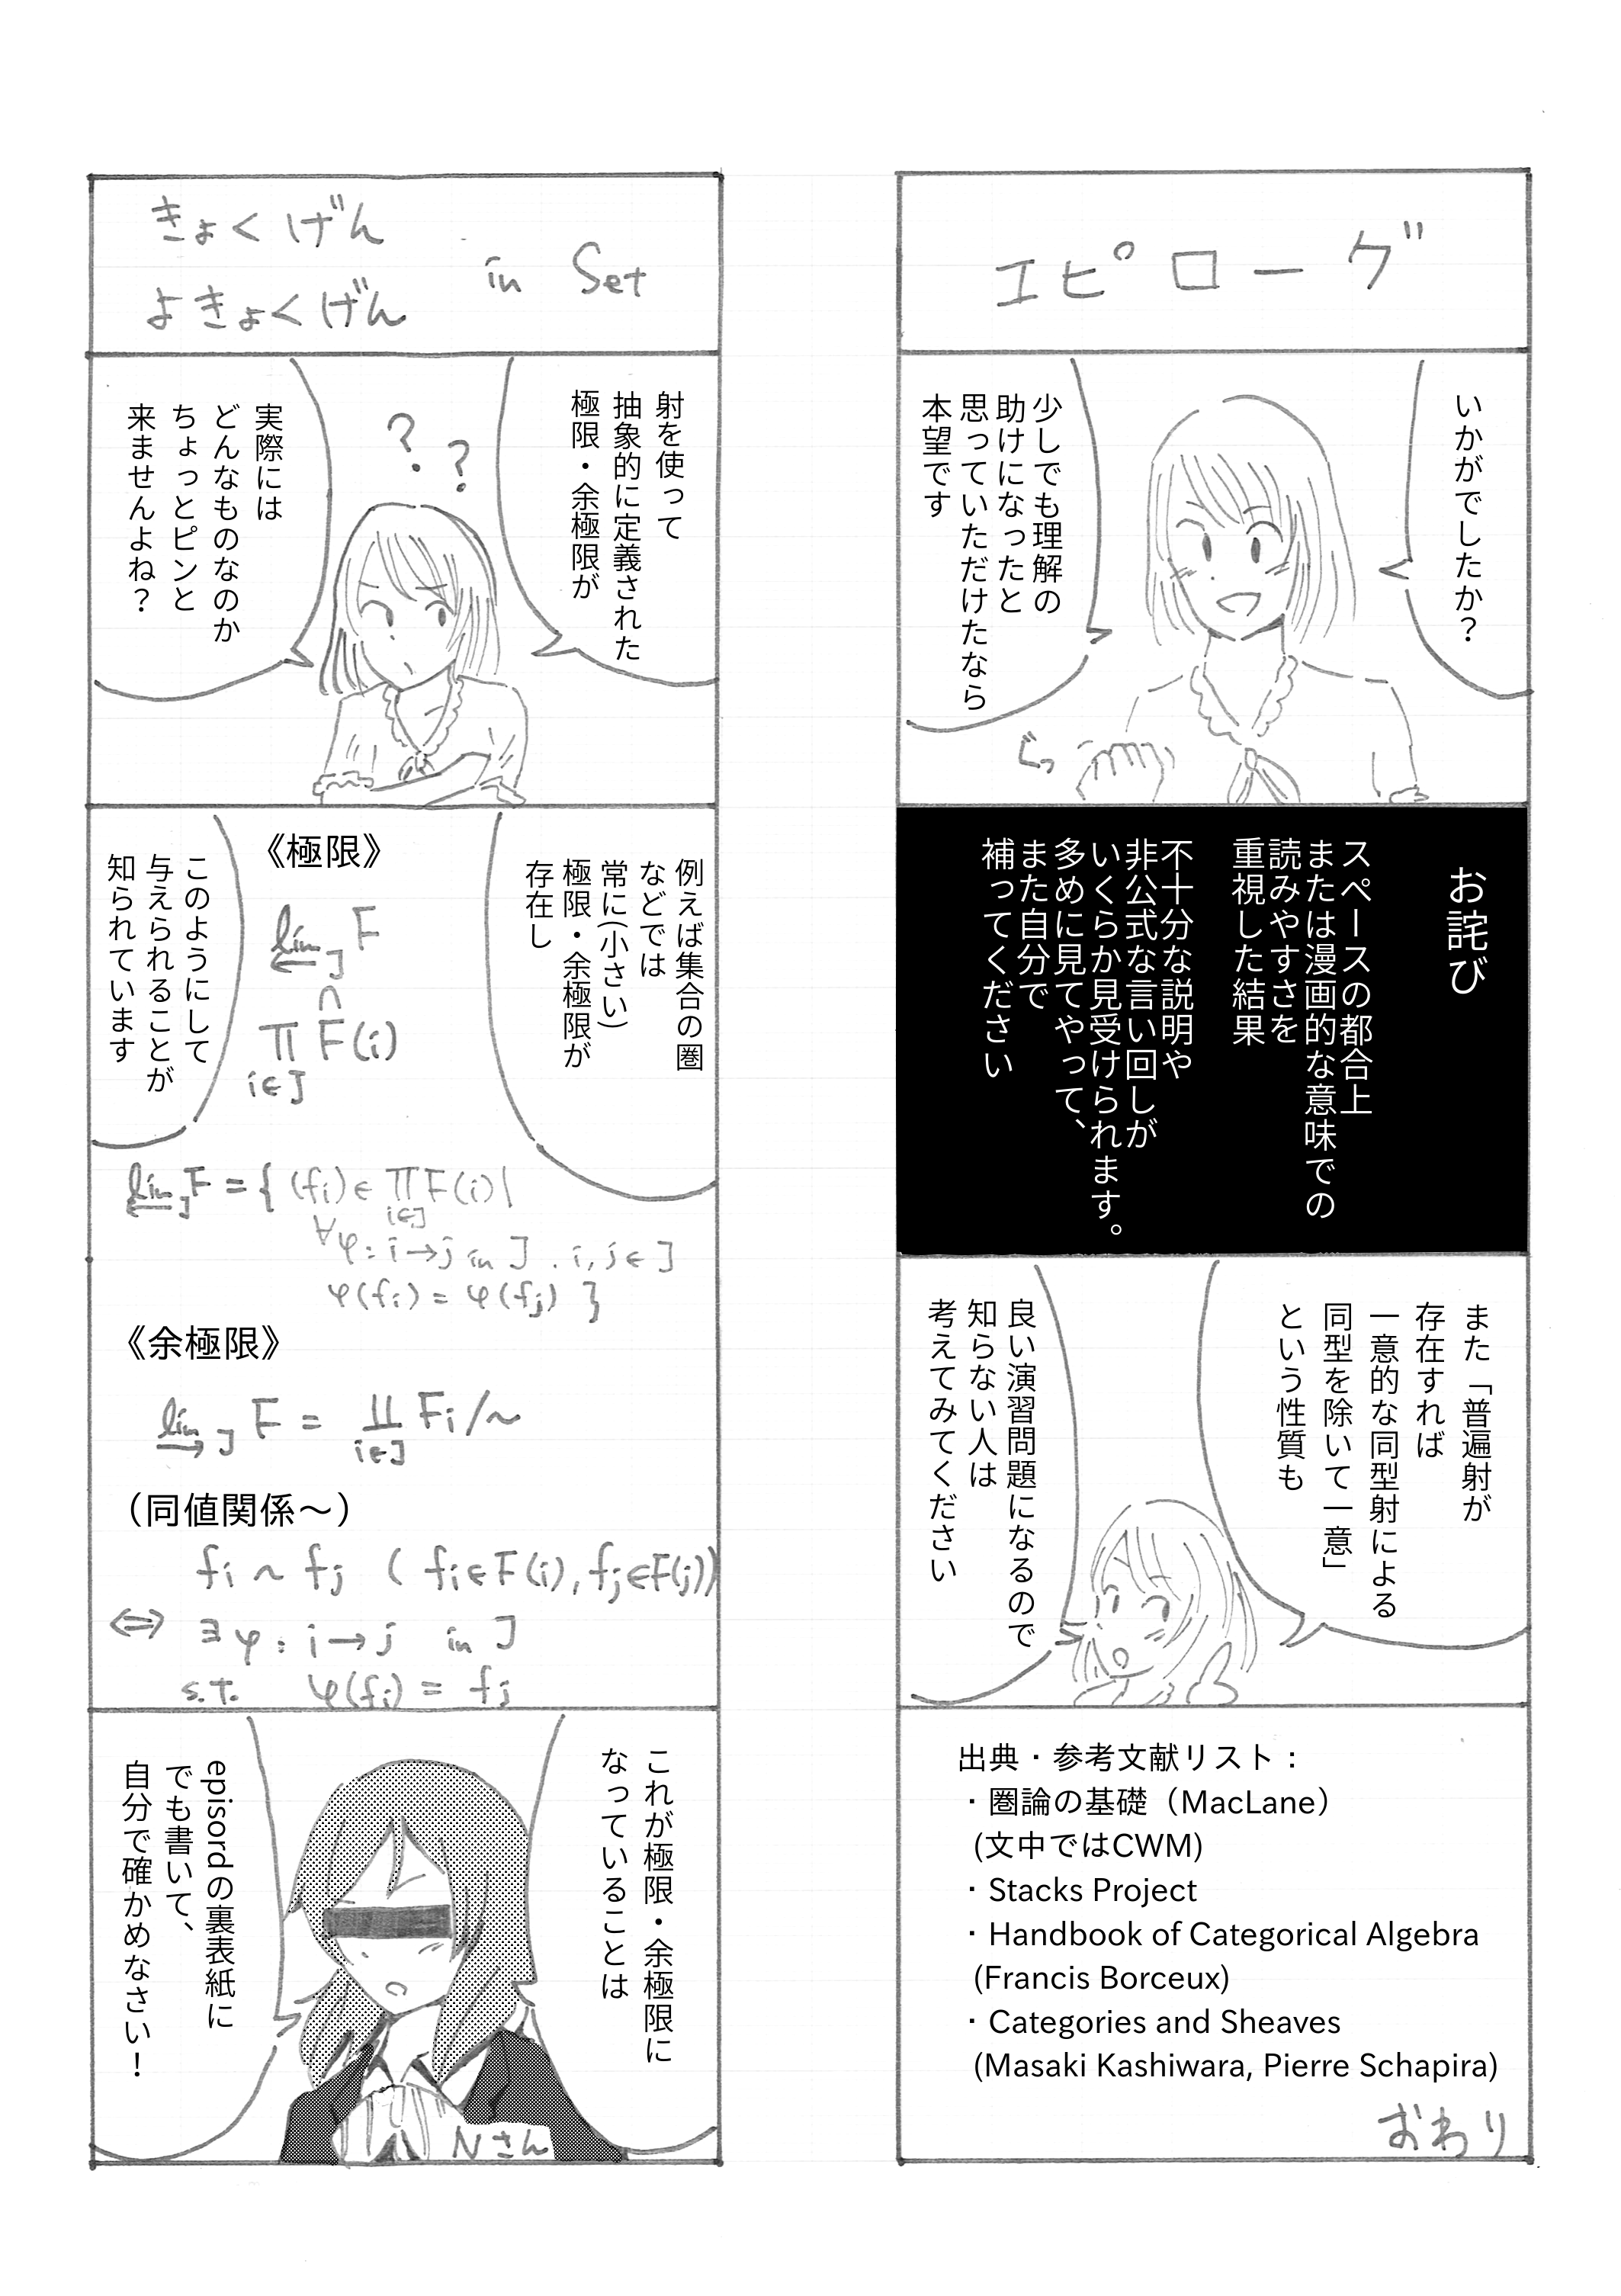
\includegraphics[width=13cm]{kobaken5.png}
%まず最初に使ったプリアンブルをここに書いてください.
%ただしコンパイルの都合上コメントアウトしてください.
%実際に確認する際は,各自の環境でmain.texにこのプリアンブルを追加してください.

%\usepackage{mathrsfs}
%\usepackage[all]{xy}
%\newcommand{\proofend}{\begin{flushright} $\blacksquare$ \end{flushright}}
%\renewcommand{\labelenumi}{(\roman{enumi})}
%\newcommand{\nkgr}{・}
%\theoremstyle{definition}
%\newtheorem{theorem}{定理}
%\renewcommand{\thetheorem}{}
%\newtheorem{defi}{定義}
%\newtheorem{thm}[defi]{定理}
%\newtheorem{lem}[defi]{補題}
%\newtheorem{cor}[defi]{系}
%\newtheorem{prop}[defi]{命題}
%\newtheorem{ex}[defi]{例}


\Chapter{代数学の基本定理でみる数学の世界(伊藤)}
% タイトル(名前)でお願いします.
% セクションは \Section \Subsection \Subsubsection で分けてください.
% 詳しくはMAY2015を参考にしてください.
\Section{はじめに}
数学科展示ますらぼにお越しいただきましてありがとうございます.
数学科とはどのようなことをやっている学科なのか一般の人に説明するのはなかなか難しく,
一般の人に端的な説明を求められるとなかなか四苦八苦してしまうところがあります.
この記事では数学科がどのようなことを勉強しているのかについて,
\textbf{代数学の基本定理}という定理を題材に出来るだけわかりやすく説明したいと思います.
この記事は第7回関西すうがく徒のつどいにおける拙講演「代数学の基本定理でみる数学の世界」を
更に詳しくして紙面化したものですので,講演に関してまとめたウェブ上の記事 \url{http://togetter.com/li/878845} も参考にしていただければと思います.
\Section{代数学の基本定理とは}
代数学の基本定理とは
\thm
次数が$1$以上の複素係数一変数方程式には複素根が存在する
\thmx
という定理です.具体的にはどういうことを言っているのでしょうか.例を見てみましょう.
\ex
$2x-4=0$というのは$1$次方程式ですが$x=2$という解を持ちます.
\exx
\ex
$ax^2+bx+c=0$というのは$2$次方程式ですが,この方程式の解の公式も中学校で習ったことでしょう.
\exx
\ex
$3$次多項式と$4$次方程式にも,極めて難解ですが解の公式というものが知られています.
これについては``カルダーノの公式''や``フェラーリの公式''で調べてください.
\exx
これらの解の公式とは\underline{具体的にバッチリと解のありかを求める}公式です.
一方で代数学の基本定理とは複素根が存在すると言っているだけなので,\underline{どこにあるかは分からないけど}\\\underline{とりあえず存在はするよ}という定理なんです.
しかし,これはどんな方程式にも解があるということを言っているのでそれは強い主張であるともいえます.
この定理は$1600$年ごろに様々な数学者によって予想され,$1800$年ごろにガウスによって証明がされました.
代数学の基本定理は高校生でも証明できるような定理なのですが,その基本的さ故に様々な証明があり,
大学$3,4$年生で習うようなことを使っても証明することができます.
この代数学の基本定理と共に大学の数学とはどのようなものなのかを見てみましょう.
\Section{大学1年生}
大学$1$年生で習う数学とは``解析学入門''と``線形代数学''の$2$つです.
どちらも数学の基礎であるとともに理系の多くの学科でも使われるものです.
\Subsection{解析学入門}
解析学入門は東大では``数学$1$''という科目名で開講されています.
微分と積分について現代数学的に学び直そうという科目です.
意識高く大学で勉強をしようと思っていた東大の$1$年生たちの多くがこの科目に打ちのめされて俗にいう五月病に羅患します.
この解析学のつまづきやすい$2$つのポイントとして,\large{$\varepsilon$-$\delta$論法}と\large{コンパクト}というものがあります.
この$2$つについて見てみましょう.
\Subsubsection{$\varepsilon $- $\delta$ 論法}
高校数学にも極限という概念はあって,$x$が$0$に限りなく近づくとか$n$が$\infty$に発散するとかいう言葉が使われています.これを厳密に定義しようというのが$\varepsilon$ - $\delta$ 論法です.
本格的な$\varepsilon$ - $\delta$ 論法に入る前に幾つか練習をしてみましょう.
\ex
ある$x$という実数の絶対値は全ての正の数$p>0$より小さいとします.これを数式で書くと以下のようになります.
\[
\forall p > 0 : \ |x| < p
\]
$\forall p$で全ての$p$についてということを言っているわけです.
ではこの$x$はどんな数なのでしょうか.$p=0.1$としてみても,$|x|$はこれより小さいです.$p=0.0001$としても$|x|$はこれより小さいです.
$p=0.000\cdots (0が2億個) \cdots 01$よりも$|x|$は小さいです.これはつまり$|x| = 0$ということです
$x$は$0$としたわけではないが,$0$になってしまった.これが現代数学の``限りなく近い''という概念をつかむのに大事な考え方です.
\exx
\ex
ある$x$という数は全ての正の数$p>0$よりも大きいとします.つまり,
\[
\forall p > 0 : \ x > p
\]
です.この$x$も具体的にはどんな数なのでしょうか.$p=1000$としてみても,$x$はこれより大きいです.$p=2億$としてみてもこれより大きいです.
これもやはり$x$は$\infty$であるということを示しているのではないでしょうか.$\infty$というのはきちんと定義されていませんが,
$x$は限りなく大きいとはこのような気分なんだなあということがイメージできます.
\exx
ではここで,$\varepsilon-N$論法というのを見てみましょう.
\defb[$\varepsilon$ - $N$ 論法]
$\lim_{n\to\infty} a_n = \alpha $\\
$\iff$
$\forall \varepsilon > 0,\  \exists N \in \N \quad \textrm{s.t.}\  \forall n \in \N,\  n > N \Rightarrow |a_n - \alpha | < \varepsilon $
\defe
突然数式がたくさん出てきて混乱したかもしれませんが落ち着いて見れば簡単です.\\
$\lim_{n\to\infty} a_n = \alpha $というのを定義しているわけです.\\
$a_n$が$\alpha$に限りなく近づくとはどういうことをなのでしょうか.\\
それは,例で見たとおり,$|a_n - \alpha|$が限りなく小さくなればいいわけです.
それを表すために,$\varepsilon > 0$というとても小さな数を$1$つ取ってきます.
それに対して,ある$N$を取ってきて$N$以降では$|a_n - \alpha | < \varepsilon$が成り立っているよとするわけです.\\
例えば,$1000$項目以降では,$|a_n - \alpha| < 0.001$が,$100000$項以降では,$|a_n - \alpha | < 0.0000000001$が成り立っていたら
どんどん近づいて行くような気がしますよね.これが限りなく近づくよ,ということを言うためにまず$\forall \varepsilon > 0$としているわけです.\\
\ex
$a_n = \frac{n+1}{n}$とすると$n \to \infty $でこれは$1$に収束します.\\
実際,$|a_n - \alpha| = | \frac{n+1}{n} - 1 | = | \frac{1}{n} |$です.\\
例えばこの$|a_n - \alpha|$を$0.01$より小さくしたい!と思えば,$N=100$としてあげれば,
$N$項目以降では$|\frac{1}{n}| < 0.01$が成り立つわけです.\\
ここでも,$|a_n - \alpha| $という差は$n$が大きくなるに連れてどんどん小さくなっていますね.
\exx
このような方法を採用するメリットとして,極限という概念がきっちりと定義されて,例えば,次のような明らかに成り立って欲しい極限の性質も厳密に証明する事ができます.
\prob
$\lim_{n\to\infty} a_n = \alpha , \lim_{n\to\infty} b_n = \beta $とする.\\
$\lim_{n\to\infty} (a_n + b_n) = \alpha + \beta , \lim_{n\to\infty} a_n b_n = \alpha\beta $
を示せ.
\probx
同様にして$\varepsilon-\delta$論法も見てみましょう.
\defb[$\varepsilon - \delta$ 論法による定義]
$\lim_{x \to a}f(x) = b$\\
$\iff$
$\forall \varepsilon > 0,\  \exists \delta > 0\quad \textrm{s.t.}\  \forall x \in \mathbb{R},\  0 < |x-a| < \delta \to |f(x)-b| < \varepsilon$
\defe
これも同様の考え方です.$x\to a\  (xがどんどんaに近づく)$のとき,$f(x) \to b\  (f(x)はどんどんbに近づく)$ということを定義しているわけです.また$|f(x)-b|$を限りなく小さくするために,$|x-a|$の幅を限りなく小さくとっているわけです.\\
またこの$\forall \exists$という並びは,どんな$\varepsilon (とても小さいイメージ)$に対してでも,いちいち$\delta (さらに小さいイメージ)$をとってくるということを表しています.
\prob
$\lim_{x\to 0} x^2 = 0$を証明せよ.$\varepsilon >0$として,$\delta = \sqrt{\varepsilon}$とすれば,$ 0 < | x | < \delta$ならば$ |x^2| < \varepsilon = \delta^2$を示せばよい. 
\probx
\Subsubsection{コンパクト}
次に第二のつまづきポイントであるコンパクトについて触れましょう.
高校数学で次のような定理があったことを思い出しましょう.
\thm[最大値最小値の定理]
$[a,b]$を有界閉区間,$f$を$[a,b]$上の実数値連続関数とする.
このとき$f$は最大値および最小値にそれぞれ少なくとも一点で到達する.
\thmx
これは高校数学では大した有り難みもない定理でしたが現代数学では重要です.
ここで重要なのは$[a,b]$が有界閉区間であるという仮定と,$f$は連続であるという仮定です.実際
\ex[非有界]
$\R$上で連続な関数$f(x)=x$は$\R$で最大値,最小値を持たない.
\exx
\ex[不連続]
$[-1,1]$上の関数.$f(x)=1/x$は最大値,最小値を持たない.
\exx
という例が示すように,有界閉区間または連続という仮定を外すとたちまちこの定理は成り立たなくなります.
この有界閉区間という概念を一般化したのがコンパクトです.
\defb[コンパクト]
$X$空間が$(点列)$コンパクトである\\
$\iff$
$X$内の任意の点列が$X$内に収束する部分列を含む
\defe
これも例を見てみましょう.
\ex
開区間$(0,1)$はコンパクトではない.なぜならば,$\{1/n\}$という数列は$0$に収束するが,この数列の部分列は$(0,1)$内の点に収束しない.
\exx
\ex
実数$\R$はコンパクトではない.なぜならば,$\{n\}$という数列は$\infty$に発散するが,この数列の部分列は$\R$内の点に収束しない.
\exx
\thm
$I \subset \R^n$がコンパクトであることと有界かつ閉であることは同値
\thmx
という風にコンパクトは有界閉区間の拡張になっているわけです.そして,
\thm
$I \subset \R^n$をコンパクト,$f$を$I$上の実数値連続関数とする.
このとき$f$は最大値および最小値にそれぞれ少なくとも一点で到達する.
\thmx
という定理が成り立ちます.こうして,$2$のポイントをおさらいしたところでその応用として代数学の基本定理を証明してみましょう.
\thm[代数学の基本定理]
次数が$1$以上の任意の複素係数一変数多項式$p(z)=a_0+a_1 z+\cdots + a_nz^n$には複素根が存在する.
\thmx
\proof[初等解析による証明]
これは杉浦光夫「解析入門1」に載っている証明です.
証明のポイントは3つ.\\
$(1)\ \lim_{|z|\to\infty}|p(z)| = \infty$\\
$(2)\ |p(z)|$はコンパクト集合上で最小値を取る.\\
$(3)\ |p(a)|>0 \Rightarrow \exists b \in \C \ s.t. \ |p(b)| < |p(a)|$(下には下がいる)
です.
\[
\lim_{|z|\to\infty}|p(z)| = \infty
\]
という意味をもう一度解釈してみましょう.
\[
\forall M \in \R \ \exists R>0 \ s.t. \  |z| > R \ \Rightarrow\  |p(z)|>M
\]
ということでした.そして$M$は任意ですから,$M=|p(0)|$として,それに対して$R>0$を一つ取り,
$K=\{ z\in\C |\ |z|\le R\}$とおけば,$K$の外では$|p(z)|>M$が成り立ちます.
つまりこの$K$の中で最小値を探せばいいいわけです.ところで$K$はコンパクトであるので
\begin{center}
$|p(z)|$は$K$上で最小値を取る
\end{center}
が言えます.最後に,
\[
|p(a)|>0 \Rightarrow \exists b \in \C \ s.t. \ |p(b)| < |p(a)|
\]
が言えて$(この証明は杉浦に譲ります)$証明終了.
\proofx
代数学の基本定理の証明は$1$年生の解析の大事な部分を使って得られるのでした.
\begin{itembox}[l]{解析学入門のまとめ}
$\varepsilon$-$\delta$論法は極限の概念を厳密化するもの.コンパクトは有界閉区間を一般化したもの.
この$2$つの概念を使って代数学の基本定理は証明できる.
\end{itembox}
\Section{大学2年生}
\Subsection{解析学続論}
大学$1$生では他に線形代数という科目を勉強しますが,この記事には関係ないので割愛します.
大学$2$年生では$1$年生で習った解析学と線形代数学の発展について学びます.
解析学では多変数の解析について学びます.ここでは線積分というものについて触れましょう.
今まで積分といえば,$\int_a^b$と言ったように区間$[a\ b]\subset \R$上での積分を考えてきましたが,
例えば,円周$\{(x,y)\in\R^2 | x^2+y^2=1\}$にそってある関数を積分したいということは数学だけでなく
多くの理系分野でよくあることです.まず曲線とは何かについて考えてみましょう.
\defb
$I\subset\R$を区間とします.$\phi:I \to \R^n$が空間曲線であるとは,一対一の連続写像であるこということである.
\defx
一対一というのは,$a\neq b \Rightarrow \phi(a) \neq \phi(b)$であるということで,つまりは自己交差をしないということです.
確かに自己交差をしなくてちゃんと繋がっていなくては曲線とはいえませんね.
\ex
$\phi:[0,1] \to \R^2$を$\phi(t)=(t,t)$で定める.これは$(0,0)$と$(1,1)$を結ぶ直線であり,空間曲線である.
\exx
\ex
$\phi:[0,2\pi) \to \R^2$を$\phi(t)=(\cos t ,\sin t)$で定める.これは単位円周です.
\exx
それではこれらの曲線にそった積分というのを次で定めます.
\defb
$f:\R^n \to \R$を関数,$\phi:I\to\R^n$を滑らかな曲線として,この曲線の像を$C$で表す.曲線$C$に沿った$f$の線積分を以下で定義する.
\[
\int_C f(x)ds := \lim_{d(\Delta)\to 0} \sum_{i=1}^N f(\phi(\xi_i)) |\phi(t_i) - \phi(t_{i-1})|
\]
ただし,ここでの$\Delta$とは区間$I$の分割$t_0 < t_1 < \cdots < t_{N-1} < t_N$を考えており$d(\Delta)$はその分割の最も大きい幅です.
\defe
これはリーマン積分の考え方を使った積分の定義であり,詳しくは$e\pi isode\ vol.3$の``積分の歩み''を参照していただきたいのですが,
基本的には高校でならった区分求積法の考え方と同じで,区分求積法はある区間を同じ幅で分割していましたが,それを好きな幅で分割して良いようにしたという話です.またこの積分は収束して以下のようにも表されます.
\prop
$f,\phi,C$を上の定義と同様とし,$I=[a,b]$となるときに次が成り立つ.
\[
\int_C f(x) ds = \int_a^b f(\phi(x))|\phi'(t)|dt
\]
\propx
\ex
$f:\R^2\to\R$を$f(x)=1$という定数関数にして,$\phi:[0,1] \to \R^2$を$\phi(t)=(t,t)$で定める.\\
このとき
\[
\int_C f(x) ds = \int_0^1 |(1,1)| dt = \int_0^1 \sqrt{2}  dt  = \sqrt{2}
\]
です.この積分は$(0,0)$と$(1,1)$を結ぶ直線の長さ$\sqrt{2}$を求めています.
\exx
\Subsection{複素解析}
(複素解析については,この$e\pi isode$にある荒田さんの記事が大変参考になります.)
代数学の基本定理の証明方法に複素解析的な方法を使ったものが有名です.
複素解析は今まで実数関数でやってきたことを複素数の範囲に拡張することによって色々な美しい結果が得られる学問です.
複素解析の主な研究対象には正則関数というものがあります.まずそれを定義しましょう.
\defb[正則関数]
$f:\C \to \C$が正則であるとは各点で微分係数を持つということである.つまり,
\[
f'(z) = \lim_{h\to 0} \frac{f(z+h) - f(z)}{h}
\]
が各$z\in\C$で収束するということである.
\defx
\rem
これだけでは普通の実数の微分可能関数と変わらないではないかと思うかもしれませんが次のようことが成り立つことに注意しなければなりません.
つまり,$h\to 0$としていますがこの$h$は複素数なので色々な$0$への近づき方をするということです.
$h=x+yi$とおいて実部と虚部に分けたとき,$y=0,x\to 0$として$0$に近づけたときこれは偏微分$\frac{\partial f}{\partial x}$になります.
一方で$x=0,y\to 0$として$0$に近づけたとき,
\[
f'(z) = \lim_{y\to 0} \frac{f(z+yi)-f(z)}{yi} = -i\frac{\partial f}{\partial y}
\]
であり,
\[
f'(z) = \frac{\partial f}{\partial x} = -i\frac{\partial f}{\partial y}
\]
が成り立つ必要があります.この関係をコーシー・リーマンの関係式といいます.
\remx
次に$\C$の部分集合として重要な単連結領域というのを定義しますが,これは``便利な領域''として考えて頂いて構いません.
\defb[単連結領域]
$D \subset \C$が単連結領域であるとは,連結な開集合であって$D$内の任意の閉曲線は$1$点にホモトピックであるようなものである.
\defx
$1$点とホモトピックであるとはこの記事の後半を参照していただきたいのですが,単連結領域とは穴がない領域をイメージしてください.
そうすると以下のように重要な定理が成り立ちます.
\thm[コーシーの積分定理と積分公式]
$D$を単連結領域とし、$f(z)$ は $D$ 上で正則である複素関数とするとき、$C$ を $D$ 内にある長さを持つ単純閉曲線とする.
\[
 \oint_C f(z) \, dz\ = 0
\]
$a$をまた$C$によって囲まれる領域に属する点とする.
\[
 f(a) = \frac{1}{2 \pi i}\int_C \frac{f(z)}{z-a}dz
\]
\[
 f^{(n)}(a) = \frac{n!}{2 \pi i}\int_C \frac{f(z)}{(z-a)^{n+1}}dz
\]
\thmx
この定理の意味とは$f(z)$が正則であれば,どんな閉曲線上で積分してもその値は$0$になるということと,
逆に$a$という一点でだけ正則でないような$\frac{f(z)}{z-a}$という関数を積分するときは$f(a)$の値のみを考えればいいよという意味です.
実際に例を見てみましょう.
\ex[コーシーの積分公式の例]
$f(z) = 1 , C = \{z\in\C | |z-a|=r\} $ のときコーシーの積分公式.\\
\[
1^{(n)}(a) = \frac{n!}{2 \pi i}\int_{|z-a|=r} \frac{1}{(z-a)^{n+1}} dz 
\]
となりますが
\[
 \int_{|z-a|=r} \frac{1}{(z-a)^{n+1}} dz =
  \begin{cases}
   \  2\pi i  \ \ (n=0) \\
   \  0 \ \ (n \ge 1) \\
  \end{cases}
\]
に他ならなりません.
\exx
正則関数がどれだけ関数に強い条件を課しているかというのは次の定理でわかります.
\thm[リュービルの定理]
複素平面全体で正則かつ有界な関数は定数関数のみ.
\thmx
\proof
\leavevmode\\
この証明は,藤本坦孝「複素解析」に載っている証明です.
証明のポイントは以下の$3$つです.\\
$(1)\ f有界つまり\forall z \in \C :\ |f(z)|\le M $かつ$f$正則を仮定する.\\
$(2)\  $仮定を満たす関数は正則より$f(z)=\sum_{n=0}^\infty c_n z^n $とべき級数展開可能\\
$(3)\ c_n$は$\forall R>0 : \ |c_n|\le \frac{M}{R^n}$をみたす.(ここでコーシーの積分公式が使われている)
\proofx
このリュービルの定理を用いて代数学の基本定理を証明する事ができます.
\proof[リュービルの定理を用いた代数学の基本定理の証明]
\leavevmode\\
この証明はLars Valerian Ahlfors「Complex Analysis」に載っている証明です.
証明のポイント:\\
$(1)\ p(z)=a_n z^n + \cdots + a_1 z+ a_0$が零点を持たないと仮定する(背理法)\\
$(2)\ g(z) = \frac{1}{p(z)}$は$\C$上で正則となる\\
$(3)\  \lim_{|z|\to\infty} |g(z)| = 0$となる.\\
$(4)\ $上から$g:$有界であることが言え,Liouvileより定数となり矛盾.
\proofx
複素解析の一つの目標として留数計算というものがあります.コーシーの積分公式では分数型の$1$点のみで正則でない関数の積分を考えましたが,
今度は他の形の正則でない点が複数ある場合でも積分計算をしてみようというというものです.
\defb[留数]
$f$が環状領域$\Delta(a,r,R) = \{z\in\C | \  r<|z-a|<R\}$で正則とする.このとき\\
\[
f(z) = \sum_{n=-\infty}^{\infty} a_n (z-a)^n
\]
という風に展開できて,これを$f$のローラン展開という.\\
特に$\Delta(a,0,R)$で正則$(a$のみ孤立して正則でない$)$とき,\\
$a_{-1}$のことを$f$の$a$での留数といい$\Res_{a} f$とかく.\\
\defx
\ex
$\frac{1}{z-c}$という関数を$|z|>|c|$でローラン展開すると.
\[
\frac{1}{z-c} = \frac{1}{z} + \frac{c}{z^2} + \frac{c^2}{z^3} + \cdots
\]
\exx
\thm[留数定理]
$D:$区分的$C^1$境界を持つ領域.$f:\overline{D}\setminus\{p_1,\cdots,p_n\}$で正則とする.
\[
\frac{1}{2 \pi i}\int_{\partial D} f(z)dz = \sum_{i=1}^n Res_{p_i} f
\]
\thmx
この留数定理とは,$f$という関数を積分する際は,$p_i$という点での留数のみを考えればいいよと言っているわけです.
留数を計算するのに便利な次の公式を紹介します.
\prop
$(1)\ z=a$に於いて$\lim_{z\to a} (z-a)f(z)$が有限確定値を持つとき,
\[
\Res_{a} f = \lim_{z\to a} (z-a)f(z)
\]
$(2)\ z=a$に於いて$\lim_{z\to a} (z-a)^m f(z)$が有限確定値を持つとき,
\[
\Res_{a} f = \frac{1}{(m-1)!} \lim_{z\to a} \frac{d^{m-1}}{dz^{m-1}} ((z-a)^mf(z))
\]
$(3)\ g,h$を正則関数として,$g(a)\neq 0,h(a)=0,h'(a)\neq 0$ならば
\[
\Res_{a} \frac{g}{h} = \frac{g(a)}{h'(a)}
\]
\propx
$\lim_{z\to a} (z-a)^m f(z)$が有限確定値を持つとき,$a$は$m$位の極であるといいますが,
$m$位の極の留数を計算するときは$(z-a)^m f(z)$という正則関数のテイラー展開を考えてあげればいいという話です.
正則関数の零点に関して次のような定理が成り立っています.
\thm[偏角の原理]
$D:$今までと同様.$f:$正則とする.
\[
\frac{1}{2 \pi i} \int_{\partial D} \frac{f'(z)}{f(z)}dz = (f\mbox{の}D\mbox{内の重複度込みの零点の個数})
\]
\thmx
\thm[ルーシェの定理]
$D:$区分的に$C^1$な境界を持つ有界領域\\
$f,g:D$とその境界上で定義された正則関数.\\
$\forall z \in \partial D :\ |f(z)-g(z)|<|f(z)|+|g(z)|$が成り立つとする.\\
このとき,$f$と$g$の零点の個数は等しい.
\thmx
ルーシェの定理は$f$と$g$の零点の個数を見たいときにその境界上のみで$f,g$の様子を考えて上げればいいという定理です.
\proof
\leavevmode\\
定理・証明ともに平地健吾先生に教えて頂きました.
証明のポイント\\
$(1)\ F_t(z) = (1-t) f(z) + t g(z)$は$0$にならない\\
$(2)\ N_t=\int_{\partial D} \frac{F_t'(z)}{F_t(z)}dz$は偏角の原理より$F_t$の零点の個数だがこれは$t$について連続.\\
$(3)\ (f$の零点の個数$)=N_0=N_1=(g$の零点の個数$)$
\proofx
%誰か良い例ください
この定理を用いて代数学の基本定理を証明する事ができます.
\proof[ルーシェの定理を用いた代数学の基本定理の証明]
\leavevmode\\

$f(z)=a_n z^n + \cdots + a_1 z+ a_0$と$g(z)=a_n z^n$とおく.\\
$|f(z)-g(z)|$は$n-1$次式,$|f(z)|+|g(z)|$は$n$次式より,\\
十分大きな円周上では$|f(z)-g(z)|<|f(z)|+|g(z)|$が成り立つ.\\
よって$f$の零点の個数は$n$個
\proofx
\prob
実はルーシェの定理まで行かなくても偏角の原理のみで代数学の基本定理を証明する事ができます.各自考えて見てください.
\probx
\begin{itembox}[l]{複素解析のまとめ}
複素解析は正則関数という性質のよいものを扱う学問.複素関数の積分は正則でない点の留数のみを見ることによってできる.
リュービルの定理は正則関数の条件の強さを表し,偏角の原理やルーシェの定理は正則関数の零点の個数を調べるものである.
これらを使って代数学の基本定理は証明できる.
\end{itembox}
\Subsection{集合と位相}
ここでは位相空間論というものについて触れましょう.今までは$\R^n$のみで連続や収束という概念を考えて来ましたが,これを任意の集合に対して
扱えるようにするのが位相空間論の一つの目標です.

\defb[位相空間]
$X$を集合とする.$X$の部分集合からなる集合$\mathcal{O}$が$X$の開集合系である.\\
$\iff (1) (U_i)_{i\in I}$が $\mathcal{O}$の族ならば,$\cup_{i\in I} U_i \in \mathcal{O}$\\
$(2)(U_i)_{i\in I}$が $\mathcal{O}$の有限族ならば,$\cap_{i\in I} U_i \in \mathcal{O}$\\
また$\mathcal{O}$に属する元を$X$の開集合といい,$(X,\mathcal{O})$を位相空間という.
また閉集合とは開集合の補集合になっているものと定義します.
\defx
このようにして任意の集合に対して好きな開集合だけを集めてきて空間の構造を与えられることができるわけです.
\ex
自然数の集合$\N$に対して次のような位相を与えることができる.\\
$(1)$\ $\mathcal{O} = \{\emptyset , \N\}$\\
$(2)$\ $\mathcal{O} = \{U\subset\N | Uは\N の部分集合\}$\\
$(3)$\ $\mathcal{O} = \{ \N \setminus I | I\subset\N は有限部分集合\} \cup \{ \emptyset \}$\\
これらの例は全て開集合系の定義を満たしていますので,これらにより$\N$を位相空間とできます.\\
$(1)$を密着位相,$(2)$離散位相,$(3)$を補有限位相と言います.
\exx
ここで収束を位相空間の言葉で書いてみましょう
\defb
位相空間$X$の点列$\{x_n\}$が$x$に収束する
\[
\iff\ \forall U :xを含む開集合 \ \exists N \in \N \ s.t.\ n \ge N \Rightarrow x_n \in U
\]
\defx
こう見てみると$U$とは$\varepsilon-\delta$のように$\varepsilon$とっていることがわかります.
つまり,位相空間とは開集合によって,集合に近いという考え方を与えているわけです.
こう考えてみると,$(1)$の密着位相は全ての点が同じ開集合に属しており,近いところにいるという意味で``密着''しています.\\
$(2)$の離散位相は,全ての$2$点は別々の開集合に入れることができるので``離散''しています.\\
ここで,集合に$(1)(3)$の場合の収束について見て見ましょう.
\ex
$x_n = n$という$\N$内の点列を考える.\\
このとき,$(1)(3)$の位相構造において$x_n$は任意の点に収束する.\\
$(1)$の場合.例えば,$1$に収束することを示してみましょう.$1$を含む開集合は$\N$だけですから,
$n \ge 1 \Rightarrow x_n \in \N$が成り立ちます.よって,$x_n$は$1$に収束します.\\
$(3)$の場合.$U$を$1$を含む開集合とします.これは$\{a_1,\cdots,a_n\}$という有限集合の補集合になっています.\\
よってこれらの最大値を$N$とおくと,$n \ge N+1 \Rightarrow  x_n \notin \{a_1,\cdots,a_n\}\ (最大値より大きいので)$が成り立つので,
\[
\iff\ \forall U :1を含む開集合 \ \exists N \in \N \ s.t.\ n \ge N \Rightarrow x_n \in U
\]
が示せました.同様にして,$x_n$は任意の点に収束することがわかります.一方で$(2)$の場合は$U=\{1\}$という開集合に対して$N$が取ってこれないので任意の点に収束しません.
\exx
次のような扱いやすい空間が定義されます.
\defb
$X:$位相空間,$A\subset X$ がコンパクトである.$\iff$
\[
A \subset \cup_{i\in I} U_i \Rightarrow \exists \{i_1,...,i_n\} \subset I s.t. \ A \subset U_{i_1} \cup \cdots \cup U_{i_n}
\]
\defx
\ex
$(1)(3)$はコンパクトである.$(2)$はコンパクトではない.
\exx

位相空間がコンパクトであるという概念については斎藤毅「はじまりはコンパクト」や斎藤毅「集合と位相」に詳しく解説されています.
また,最初に定義した点列コンパクトとコンパクトという概念は一致します.
\defb
$X$がハウスドルフ空間である.$\iff$\\
$x,y \in X , x\neq y \Rightarrow \exists U:x\mbox{の開近傍} ,\exists V:y\mbox{の開近傍} \ s.t. \ U \cap V = \emptyset$
\defx
\ex
$(1)(3)$はハウスドルフではない.$(2)$はハウスドルフである.
\exx
また連結という概念も位相空間の言葉を使って定式化することができます.
\defb
$X$が連結空間である.$\iff$\\
$X$の部分集合で開集合かつ閉集合であるようなものは,$\emptyset$と$X$のみ.
\defx
\ex
$(0,1) \cup (2,3)\subset\R$は連結空間ではない.\\
実際,区間$(0,1)$は開集合でかつ,$(2,3)$という開集合の補集合になっているので閉集合です.\\
これはこの区間が繋がっていないことによって起こる結果です.
\exx
ここで連続写像の概念も極めてシンプルに一般化されます
\defb
$f:X\to Y$が連続写像である.$\iff$\\
$U \subset Y$が開集合ならば$f^{-1}(U) \subset X$は開集合.
\defx
次の定理は,連続写像の性質を表すとともに,最大値最小値の定理と中間値の定理を一般化したものとも言えます.
\thm
$X,Y$を位相空間として,$f:X\to Y$を連続写像とする.\\
$(1)$$A\subset X$がコンパクトならば$f(A)\subset Y$もコンパクトである.\\
$(2)$$A\subset X$が連結ならば$f(A)\subset Y$も連結である.\\
\thmx
\rem
一方で\\
$(3)A\subset X$が開集合ならば$f(A)\subset Y$も開集合である.\\
$(4)A\subset X$が閉集合ならば$f(A)\subset Y$も閉集合である.\\
はどちらも一般には成り立ちません.これらが成り立つ写像をそれぞれ.開写像,閉写像といいます.
\remx
\proof[位相空間論における代数学の基本定理の証明]
この証明は斎藤毅「集合と位相」に載っている証明です.\\
$f:\C \to \C$を多項式が定める写像とすると,\\
正則関数の一般論から$f$は開写像であることが言える.\\
また$\C$の一点コンパクト化である$\C P^1$を考えることにより,$f$は閉写像であることがわかります.\\
よって,$\C$は連結空間で$f(\C)\subset\C$は開かつ閉であり,空集合でないので$f(\C)=\C$がいえます.\\
つまり,この多項式には$0$点が存在します.
\proofx
\begin{itembox}[l]{集合と位相のまとめ}
位相空間とは,集合に開集合とはなんであるかを定めることにより元の遠近感を定めたもの.これにより連続関数を定義できる.
また性質の良いコンパクト空間やハウスドルフ空間や連結空間というものがあり,これらの性質により代数学の基本定理は証明できる.
\end{itembox}
\Section{大学3年生}
\Subsection{多様体}
多様体とは位相空間の中でも特に重要なもので,幾何学の主な研究対象です.
\defb[多様体]
$M:$が$n$次元の$(C^\infty 級)$多様体であるとは$M$がハウスドルフ空間であり,次のような開近傍$U_i$と同相写像$\phi_i : U_i \to \phi_i(U_i) \subset \R^n$が存在することである.\\
\[ \bigcup_i U_i = M \]
$U_i \cap U_j \neq \emptyset$のとき,次の座標変換がが$C^\infty$級である.
\[
\phi_i \circ \phi_j^{-1} | _{\phi_j(U_i\cap U_j)} :\phi_j(U_i\cap U_j) \to \phi_i(U_i\cap U_j)
\]
\defx
突然仰々しい定義が出てきましたが,多様体の$2$目の性質は局所ユークリッド的と言われるものです.
つまり,位相空間で連続写像については考えることが出来ましたが,微分を考えることはまだ出来ません.
そこで,位相空間のある一部を見てあげればそれはユークリッド空間であるとみなせるものを多様体としたのです.
つまり,多様体は好きなところに座標を入れることができ,かつ好きな用にいれた座標はちゃんとうまく合わさっているよというのがこの定義です.
幾何学の主な対称と言いましたが,例えば有名なポアンカレ予想は多様体に関する次のような定理です.
\thm[ポアンカレ予想]
\leavevmode\\
$M$多様体,$M$と$S^n$がホモトピー同値ならば$M$は$S^n$と同相である\\
$n=2$については$2$次元多様体の分類は$20$世紀はじめに知られており,
$n=3$コンパクトかつ単連結ならば$3$次元多様体は$S^3$と同相である.ということがポアンカレによって予想されました.\\
$n\ge 5$のときはスメールが解決,$n = 4$はフリードマンが解決,$n=3$のときはペレルマンが解決しました
\thmx
このように,数学の一つの目標にある概念を\underline{分類}するというものがあります.
分類することによって,今まで雑然と広がっていた世界が綺麗に掃除され見通しよくなるというのが数学の$1$つの仕事です.
では多様体での微分について定義しましょう.
\defb
多様体 $M_1, M_2$ を考える.写像 $F : M_1 \to M_2$ が $C^\infty$級であるとは、$F(x) \in M_2$ のまわりの座標近傍 $(V,\psi), F^{-1}(V)$ に含まれる$x\in M_1$ のまわりの座標近傍 $(U, \phi)$ に対して、
$\psi \circ F \circ \phi^{-1} : \phi(U) \to \psi(V )$が $C^\infty$ 級となることである。
\defx
ユークリッド空間内の多様体のみを考えて$f:M\to N$,$M\subset\R^k,N\subset\R^l$の微分を考える.\\
\[
df_x = (\frac{\partial f_i}{\partial x_j}):\R^k\to\R^l
\]
という行列で定める.\\
\defb
$x\in M$が正則点 $\iff df_x$が全射.\\
$x\in M$が特異点 $\iff df_x$が全射でない.\\
$y\in N$が正則値 $\iff f^{-1}(y)$が全て正則点.\\
$y\in N$が臨界値 $\iff f^{-1}(y)$が特異点を元として含む.\\
\defx

\proof[多様体論を用いた代数学の基本定理の証明]
\leavevmode\\
この証明はJohn Willard Milnor ``Topology from the Differentiable Viewpoint''に載っている証明です.
証明のポイント\\
$(1)\ p(z):\C\to\C$を今までどおりの多項式とする.\\
$(2)\ h:S^2\to\C$というステレオグラフィック射影によって,\\
$(3)\ h^{-1}\circ p \circ h : S^2 \to S^2$を定める.\\
$(4)\ f$が$C^\infty$級写像であることを示す.\\
$(5)\ f$は有限個の臨界点しか持たない.\\
$(6)\ f$の球から正則値の集合は有限を除いたものなので連結.\\
$(7)\ \# f^{-1}(y)$は開近傍上で定数であるので常に0でない.\\
\proofx
\begin{itembox}[l]{多様体のまとめ}
多様体とは位相空間の中でも好きなところに座標を入れてユークリッド空間のように扱えるものである.これにより
多様体の構造が入っている集合には連続写像だけでなく写像の微分を定義することが出来た.
多様体とは幾何学の基本的な研究対象である.また多項式をコンパクトな多様体$S^2(球面)$間の写像であるとしてその臨界値を見ることにより代数学の基本定理は証明できる.

\end{itembox}
\Subsection{群論}
代数学が扱う対称として基本的でシンプルなものが群です.群は集合に掛け算のみが入ったものを考えており,
例えば今まで習ってきた,整数や実数や群といったものは全て群です.群の定義は以下の様なものです.
\defb
集合$G$が群であるとは,$G$上の二項演算が$x,y,z\in G$に対して以下を満たすことである.\\
$\rm (i)$ $(xy)z=x(yz)$\\
$\rm (ii)$ $\exists e \in  G \ s.t. \ xe=ex=x$\\
$\rm (iii)$ $\forall x\in G \ \exists x^{-1} \in G \ s.t. \ x x^{-1} = x^{-1} x= e$\\
さらに,$xy=yx$を満たすとき$G$をアーベル群という.\\
\defe
また群の部分集合にも同じ演算の構造が入る場合に部分群といいます.つまり次のような定義です.
\defb
部分集合$H\subset G$が\\
$\forall x,y \in H: \ xy\in H$,\ \ $\forall x\in H:\ x^{-1} \in H$,\ \ $e\in H$\\
を満たすとき$H$を$G$の部分群という.
\defe
また部分群の中で扱いやすいものを定義します.
\defb
$N\subset G:$部分が正規部分群である\\
$\iff \ \forall g\in G : \ gNg^{-1} \subset N$
\defe
例えばアーベル群では全ての部分群は正規部分群です.
\defb
群$G$,$G'$があったとして,$f:G\to G' \  \forall x,y \in G \ f(xy)=f(x)f(y)$をみたす$f$を群準同型写像という.\\
特に$f$が準同型で全単射であるとき,同型写像であるという.
\defe
ここで群論で重要なシローの定理について触れておきましょう.
\defb
$G:$有限群,$p$:素数とする.$G$が$p$群$\iff\ |G|$が$p$のべき乗個.\\
$G$の部分群でかつ$p$群であるものを$p$部分群.\\
$|G|=p^e m, m,p$は互いに素なとき,\\
元の個数が$p^e$個の群をシロー$p$群という.
\defe

\thm[シローの定理]
$G:$有限群,$p$:素数とする.\\
$\rm (I)$シロー$p$部分群が存在する.\\
$\rm (II)$$(p\ $シロー部分群の個数$)\equiv\ 1 \bmod p$\\
$\rm (III)$$\forall P:シローp$群,$\forall Q:p$部分群,$\exists x\in G\  s.t. \ Q\subset xPx^{-1}$
\thmx
これは有限群を分類する際にとても便利な定理です.
\Subsection{ガロア理論}
ガロア論とは,体という四則演算が入った集合の拡大を考える理論で,体の拡大とそのガロア群を対応させることができるという理論です.
\defb
$K \subset L$に体の構造であるとき,$L$は$K$の拡大であるという.
\defx
\defb
$L$の同型で,かつ$K$上では恒等写像なもの全体を$\Aut_K(L)$とかく.
$\# \Aut_K(L)=[L:K]$のとき$L$は$K$のガロア拡大であるといい,$\Aut_K(L)$をガロア群という.
\defx
\ex
\[
[\C:\R]=2,\Aut_\R(\C) = \{\sigma_1,\sigma_2\}
\]
ただし,$\sigma_1$は恒等写像,$\sigma_2$は複素共役写像である.
\exx
\thm
$L/K$ を有限次ガロア拡大,$G$ をそのガロア群とする.
$(1)L/K$ の中間体 $M$ と $G$ の部分群 $H$の間に次の一対一対応がある:
\[
M \rightarrow G(L/M) , F(H) \leftarrow H
\]
$(2) M$ と $H $が対応するとき,$L/M$ はガロア拡大で $H$はそのガロア群である.
そして
\[
[L : M] = |H|, [M : K] = |G : H|
\]
$(3) M$ と $H$ が対応するとき,$M/K$がガロア拡大であることと$H$ が$G$ の正
規部分群であることは同値である.さらにこのとき
\[
G(M/K) \cong G/H. 
\]
\thmx
このガロア理論を用いても代数学の基本定理を証明する事ができます.
\proof[Galois理論による証明のポイント]
\leavevmode\\
雪江明彦「代数学2 環と体とガロア理論」に同様の証明が載っています.\\
$(1)\ K/\C$を有限次拡大とする.(背理法)\\
$(2)\ K/\R$は正規拡大であるとして一般性を失わない.\\
$(3)\ K/\R$はGalois拡大になる.\\
$(4)\ G:=Gal(K/R)$とする,$H\subset G$を2-Sylow群とすると,これに対応する拡大は奇数次拡大で,$\R$そのものしかない.\\
$(5)\ [K:\C]>1$で$2^n$であるとすると,$Gal(K/\C)$が2-群になって,$\C$が二次拡大をもつことになる.\\
\proofx
\begin{itembox}[l]{代数学のまとめ}
群論とは集合に積の構造のみを入れて考えるシンプルな学問である.
ガロア理論は体という四則演算のできる集合の拡大とこの群論を結びつける理論である.
ガロア理論により代数学の基本定理は証明できる.
\end{itembox}
\Subsection{代数トポロジー}
多様体論では微分同相という同値関係で位相空間を分類しましたが,代数トポロジーはホモトピー同値という関係でもって位相空間を分類します.例えば,コップの表面とドーナツの表面はホモトピー同値というように,我々の考える``同じ''よりも更にゆるい考えかたでものを分類します.一方で,球面とドーナツの表面はホモトピー同値ではありません.これは``穴の数''に起因しています.この穴という概念を高次元化してみるのがホモロジー群です.
\defb[ホモトピー]
$f,g:X\to Y$という連続写像ががホモトピックであるとは,\\
連続写像 $F : X \times [0, 1] \to Y$であって,すべての $x \in X$ について$ F(x, 0) = f(x), F(x, 1) = g(x) $をみたすものが存在することをいう.つまり,$F_t :X\to Y$という$t$によってパラメータ付された関数が存在して,
$t=0$では$f$と一致し,$t=1$では$g$と一致するようにできるという意味である.これを$f\simeq g$と表す.
\defx
難しいような定義が出てきましたが,$f,g$がホモトピックであるとは,$f$をじわじわと動かしていくと$g$になるというイメージです.
\defb[ホモトピー同値]
$X,Y$という位相空間がホモトピー同値であるとは,\\
$f:X\to Y$と$g:Y\to X$という連続写像が存在して,$g \circ f \simeq 1_X$,$f \circ g \simeq 1_Y$とできることである.
\defx
ここで,空間が等しいということを各学問がどのように見ているかという事を見てみましょう.
\defb
$X,Y$という集合が,集合として同等であるとは,\\
$f:X\to Y$と$g:Y\to X$という写像が存在して,$g \circ f = 1_X$,$f \circ g = 1_Y$とできることである.
\defx
\defb
$X,Y \subset \C$が双正則であるとは,\\
$f:X\to Y$と$g:Y\to X$という正則写像が存在して,$g \circ f = 1_X$,$f \circ g = 1_Y$とできることである.
\defx
\defb
$X,Y$という群が群として同型であるとは,\\
$f:X\to Y$と$g:Y\to X$という群準同型が存在して,$g \circ f = 1_X$,$f \circ g = 1_Y$とできることである.
\defx
\defb
$X,Y$という位相空間が,同相であるとは,\\
$f:X\to Y$と$g:Y\to X$という連続写像が存在して,$g \circ f = 1_X$,$f \circ g = 1_Y$とできることである.
\defx
\defb
$X,Y$という多様体が微分同相であるとは,\\
$f:X\to Y$と$g:Y\to X$という$C^\infty$級写像が存在して,$g \circ f = 1_X$,$f \circ g = 1_Y$とできることである.
\defx
このようにして,数学という学問はある集合がまず等しいという概念を定義します.そうして,等しい物を集めて,違うものは違うものに分類します. その分類に必要になるのが\underline{不変量}というものです.不変量とは,
\[
X と Y が等しい \Rightarrow XとYの不変量が等しい
\]
が成り立つものです.このとき対偶として
\[
 XとYの不変量が等しくない \Rightarrow X と Y が等しくない
\]
が成り立ちます.こうやって,不変量をみることによって,ある$X$と$Y$が等しくないかどうかということが判別できます.
話が大きくそれましたが,代数トポロジーにおける不変量としてホモロジー群というものがあります.
\defb
空間$X$を$q$次ホモロジー群$H_q(X)$に,連続写像$f:X\to Y$をホモロジー群間の準同型$f_* : H_q(X) \to H_q(Y)$に対応させる.
このとき,次のような性質を満たすようにできる.\\
$(1):$空間$X$での恒等写像は,ホモロジー群$H_q(X)$での恒等写像に対応する.\\
$(2):$$f:X\to Y,g:Y\to Z$という連続写像があるとき,$g\circ f$は$(g\circ f)_* = g_* \circ f_* :H_q(X) \to H_q(Z)$が成り立つ.
つまり位相空間での関係を保ちます.かつホモロジー群は不変量となっている.つまり,
$(3):$$X,Y$がホモトピー同値ならば,$H_q(X) \cong H_q(Y)$という同型成り立つ.
\defx
このホモロジー群が実際にあることを証明するのは少々手間がかかりますが,このような性質を満たすようなものが存在するとして
色々な結論を導くことが出来ます.例えば,$S^n$のホモロジー群と言うのは,幾つかの公理を加えるだけで簡単に証明できます.
\thm
$S^n=\{x\in\R^{n+1} | |x|=1\}$とすると,$\Ho_k S^n = \Z\  (k=0,n)$,$\Ho_k S^n = 0\  (k\neq 0,n)$
\thmx
\thm
$f:S^n \to S^n$を写像とすると,これは$f_*:\Ho_n(S^n)\to \Ho_n(S^n)$を引き起こす.\\
これは$\Z$間の準同型であるので,$f_*(x) = kx$とおけて,この$k$を$\deg(f)$と置いて,写像度という.
\thmx
\prop
写像度は次のような性質を満たす.\\
$\rm (i)$$\deg(id)=1$\\
$\rm (ii)$$\deg(f\circ g) = \deg(f)*\deg(g)$\\
$\rm (iii)$$f \simeq g \Rightarrow \deg(f) = \deg(g)$\\
\propx
ところで,この写像度というのは,回転数とも呼ばれ,$f$の定義域が単位円を一周するとき,$f$の像は単位円を何周するかということを表しています.
\proof[代数トポロジー的な代数学の基本定理の証明]
\leavevmode\\
この証明は,Albrecht Dold「Lectures on Algebraic Topology」に載っている証明です.
証明のポイント\\
$(1) \ \hat{p}:S^1\to S^1 ; z \to \frac{p(z)}{|p(z)|}$により定める.\\
$(2)\ |z|\le 1$ で 零点を持たないならば$\deg \hat{p} = 0$をしめす\\
$(3)\ p_t(z) =  \frac{p(tz)}{|p(tz)|}$による.\\
$(4)\ |z|\ge 1$ で 零点を持たないならば$\deg \hat{p} = n$.\\
$(5)\ p_t(z) =  \frac{t^kp(z/t)}{|t^kp(z/t)|}$による\\
\proofx
ここまでできるだけ丁寧に説明することを心がけてきましたが,紙面の都合上これ以降は概略をのべるのみにします.
\Subsection{微分幾何学}
\defb
$\{g_p\}_{p\in M}$がRiemann計量である.\\
$\iff \ (1)g_p : T_p M \times T_p M \to \R $は内積.\\
$(2)s_1,s_2:U\to TM:$切断とすると,$g_p(s_1(p),s_2(p))$は$C^\infty$級・
\defe
\thm
$M$:境界つきコンパクトRiemann多様体. $K$を$M$のガウス曲率. $k_g:\partial M$の測地曲率.
\[
\int_M K\;dA+\int_{\partial M}k_g\;ds=2\pi\chi(M)
\]
\thmx
\proof[微分幾何学による代数学の基本定理の証明]
\leavevmode\\
この証明は \url{http://arxiv.org/pdf/1106.0924.pdf} に載っている証明です.
証明のポイント\\
$p(z)$が零点を持たないと仮定する.\\
$p^{*}(z) = z_np(1/z) = a_0z_n + a_1z{n-1} + \cdots + a_n$として, $f(z)=p(z)p^*(z)$とする.\\
$f(\tfrac{1}{w}) = p(\tfrac{1}{w})p^*(\tfrac{1}{w}) = w^{-2n}p^*(w)p(w) = w^{-2n}f(w)$\\
$w\in \C :\ g=\frac{1}{|f(w)|^{\frac{2}{n}}}\,|dw|^2$\\
$w\in \hat{\C} \setminus \{0\}:\  g=\frac{1}{|f(1/w)|^{\frac{2}{n}}}\,|d(1/w)|^2$ とする\\
$\frac{1}{|f(w)|^{\frac{1}{n}}}\,K_g=\frac{1}{n}\Delta \log|f(w)|=\frac{1}{n}\Delta \text{Re}(\log f(w))=0$
$\int_{\mathbf{S}^2}K_g=4\pi$により矛盾.
\proofx
\Subsection{確率論}
\proof[確率論による代数学の基本定理の証明]
この証明はL. C. G. Rogers, David Williams「Diffusions, Markov Processes, and Martingales: Volume 1, Foundations」に載っている証明です.
証明のポイントは.
$(1)\ (B_t:t \ge 0)$をブラウン運動とする.\\
$(2)\ f(z) = 1/p(z)$とおくと,これは正則で,$z\to\infty$で$0$に収束する.\\
$(3)\ \alpha < \beta$として$\{\Real f \le \alpha\}$と$\{\Real f \ge \beta\}$は開集合を含む.\\
$(4)\ f(B_t)$はマルチンゲールの収束から,$f(B_t)\to f(B_\infty)$に$L^1$収束する\\
$(5)\ $一方でこれはブラウン運動の再帰性に矛盾する.\\
\proofx
\Section{参考文献}
これまで様々な分野を紹介してきましたが,それぞれの分野についてもし興味が涌いたならば是非書店や図書館に行って,本物の数学に触れてみてください.各証明に乗せている本はどれも其の分野の面白い本なので参考になると思います.



\backmatter
%\Chapter{編集後記}
\thispagestyle{empty}
\vspace*{10zw}
\vfill

\parindent=0pt
\begin{picture}(110,1)
\setlength{\unitlength}{1truemm}
\put(5,2){\Large\textbf{$e^{\pi i}sode$ Vol.4 !!!volを変える!!! }} 
\thicklines
\put(0,1){\line(2,0){110}}
\thinlines
\put(0,0){\line(2,0){110}}
\end{picture}

\small{2016年11月25日発行!!!変更する!!!}\\
 \normalsize{著 者・・・・・東京大学理学部数学科有志}\\
 \normalsize{発行人・・・・・!!!名前を書く!!!}\\
\begin{picture}(100,1)
\setlength{\unitlength}{1truemm}
\thinlines
\put(0,1){\line(2,0){110}}
\thicklines
\put(0,0){\line(2,0){110}}
\put(0,-5){\small{\copyright  Students at Department of Mathematics,The University of Tokyo 2016 Printed in Japan}}
\end{picture}


\end{document}
